\documentclass{DeustoFDP}
\emergencystretch=1em % this is for using emergency stretches in overfulls
\usepackage[toc, acronym, nomain]{glossaries}
\usepackage{eurosym}
\usepackage{verbments}
\listofpyglistingsname{Algorithm Index}

\hypersetup{
	pdfauthor={Iban Eguia Moraza},
	pdftitle={Remote robotic experiment integration in a game platform to promote STEM in young people},
}

\bibliography{bibliography}
\makeglossaries
\chapter*{Acronyms}
\addcontentsline{toc}{chapter}{Acronyms}

\begin{itemize}
	\item \textbf{STEM}: Science, Technology, Engineering and Mathematics

	\item \textbf{GOLC}: Global Online Laboratory Consortium

	\item \textbf{MIT}: Massachusetts Institute of Technology

	\item \textbf{VISIR}: Virtual Instrumentation Systems In Reality

	\item \textbf{IDE}: Integrated Development Environment

	\item \textbf{API}: Application Programming Interface
\end{itemize}


\begin{document}

\frontmatter
\pagestyle{plain}

\begin{titlepage}
  \newgeometry{left=0cm,right=0cm,bottom=0cm,top=0cm}\thispagestyle{empty}
  
\includegraphics{fig/frontpage_comp}
  \restoregeometry
\end{titlepage}
\cleardoublepage

\chapter*{Abstract}

Responding to the strong growing demand of new learning tools, a new learning experience is
presented, based on remote laboratories. This project tries to create what to the best of our
knowledge will be the first game platform based on remote laboratories. This will introduce young
students between 10 and 18 years old to \acrshort{stem} (\acrlong{stem}) in an enjoyable way.

The game platform will be divided in two main scenarios. The first of them will be a trivial type
game, where the user will be able to control a robot in a labyrinth and answer some questions that
will give points to the user. Winners will be given a prize. Moreover, in this scenario, a
psychological experiment will be performed, aiming to help in the fight against pseudoscience.

The second scenario will be a service in which the user will be able to program the robot from a
visual \acrshort{ide} (\acrlong{ide}). This will teach students the basics of programming by letting
them use blocks to program the robot and see the result.

\vspace{2em}

{\Large\bfseries\sffamily Keywords}
\vspace{3\medskipamount}

Remote Laboratories, WebLab-Deusto, Serious Games, Psychology, Visual Programming


\cleardoublepage\tableofcontents
\cleardoublepage\listoffigures
\cleardoublepage\listoftables
\cleardoublepage\listofpyglistings

\mainmatter
\pagestyle{phdthesis}

\chapter{Introduction}

This project aims to create a complete game experiment using a remote laboratory. At our best of our
knowledge, there is no game that uses remote laboratories as a platform to provide a resource in the
game, so this project aims to create the first game experience ever in a remote laboratory platform.
Moreover, it has been sponsored by the \acrshort{fecyt} (\acrlong{fecyt}) foundation's ``Ciencia
remota'' project, where this project will be deployed in museums.

We will have to develop the game using the WebLab-Deusto platform, using their hardware and their
software libraries, and we will have to integrate the game with the robot Romie in its labyrinth.
For that, we will have to learn and use many technologies, learn to use the WebLab-Deusto's network
and create a game that could be used by dozens of people.

Taking that into account, we can see how this project will confront some big challenges:

\begin{itemize}

\item Integrate hardware elements with software interface to create a game that will be used by
young students to play an learn.

\item Use the available resources of a platform never before used as a game platform: remote
laboratories.

\item Design and develop a game that would use real hardware for the gaming experience available
at all times.

\item Demonstrate the viability of the game and the reliability of the platform in real events with
users playing.

\item Learn and use the tools and libraries provided by WebLab-Deusto.

\end{itemize}

Furthermore, this project does not only try to create a game platform. Together with the psychology
laboratory of the University of Deusto, Labpsico~\cite{labpsico_web}, we will develop a complete
experience to fight against pseudoscience and gather valuable data from the experiment. We will use
the same game platform to integrate the psychological experiment they will provide us so that users
completing the psychological experience will receive better starting scores in the game.

This task in itself carries many challenges that we will have to solve:

\begin{itemize}

\item Work in an interdisciplinary environment with psychologists to design the software
integration.

\item Integrate a complete psychology experiment in a game using remote laboratories.

\end{itemize}

This challenges will need good group work skills as well as good communication skills, since we will
need to understand each others to develop the best possible solution and integrate it with the
current University of Deusto's remote laboratory platform, WebLab-Deusto.

Moreover, and since WebLab-Deusto~\cite{weblab_web} is part of DeustoTech
Learning~\cite{dtlearning_web}, the department of DeustoTech~\cite{deustotech_web} that creates
learning tools, we decided that we should create a learning experience based on the robot. This will
be one of the key parts of the project, since we do not currently have an experiment for young
students to program robots in WebLab-Deusto.

That will be accomplished using a visual programming environment that will be integrated in the
WebLab-Deusto platform where students will be able to program the robot using blocks with the latest
technologies. All this visual programming environment will be usable from the web interface of
WebLab-Deusto, with its queue and priority management.

Of course, this new scenario proposes more challenges that will have to be solved:

\begin{itemize}

\item Research about visual programming technologies and decide which to use.

\item Learn and use a new technology to create a visual programming environment.

\item Connect the environment with the robot, taking into account that it cannot break previous
developments.

\item Control the code execution to avoid security issues and acknowledge the user in eventualities.

\end{itemize}

These three scenarios will be the ones developed in this project. They will show many of the learned
abilities in the university and they will require further learning to be able to develop the
project.

In this document this project is presented. We will first take a look to the background of the
project, where we will see what other technologies and platforms exist in the world, and the
rationale for the project.

We will then define the objectives and the scope of the project, where we will define the project
perfectly and explain how the project will be developed. Finally we will show the organizational
structure of WebLab-Deusto, where the project will be developed.

After that, we will do the planning of the project, where we will be able to see the development
dates and workloads, as well as the Gantt and precedence diagrams. Then we will have the budget of
the project.

After the planning, we will start with the development of the project itself. This section will be
divided into three subsections, one for each of the scenarios of the project. The first of them will
show the game development, the second one will show the Labpsico experiment integration and the last
one will show the visual programming interface development. Each of them will explain the
requirements, the design and the deployment, along with the testing and issue management. Each of
them will have a small user manual to explain how to use them.

Once the project has been explained, we will start with the development section, where we will first
analyze the technologies we will use for this project. We will go through all the different aspects
of the software, from the embedded computers, servers and all the software technologies needed for
the development of the client and server sides. We will also research on the hardware technology
used.

Finally, we will explain the conclusions and results of this project, and we will think on some
future developments. We will show the data of all the uses of the game to show the viability of the
project.

\chapter{Background and Rationale}

\section{Background}

This project aims to create a serious game based on a robot in a remote laboratory. Moreover, it
aims to create a complete visual programming experience to teach the basics of programming. Thus,
in this state of the art, We will cover the three main topics that the project uses as a base and we
will deepen into them.

\subsection{Remote Laboratories}

Remote laboratories are usual laboratories, with the peculiarity that they can be accessed through
the Internet~\cite{remote_labs}. They give students the option to use the laboratory from home even
when the university or school is closed. This means that the students are able to do their homework
or experimentation using the equipment at their school or university without the need for them to be
physically there.

Currently they are becoming more popular due to the competitive advantage they can give to schools
and universities. Since there is no need for the student to be physically in the laboratory, the
laboratory does not need to be physically in the school or university, giving the option to share
laboratories between institutions and thus giving important economic benefits without reducing
the practice time of the students, or even increasing it.

Therefore, remote laboratories can be really helpful in teaching main concepts about science and
technology. The next laboratories are the most known ones that are working with science and
technology.

\subsubsection{Global Online Laboratory Consortium}

The \acrlong{golc} or \acrshort{golc} is an organization that focuses on the promotion of the
development of remote laboratories for educational use. They commonly promote remote laboratories
through conferences~\cite{golc1st}. They also support and encourage the sharing of these
laboratories between institutions.

\begin{figure}[!htbp]
	\centering
	
\includegraphics[width=0.35\textwidth]{fig/golc-award}
	\caption{\acrshort{golc} Online Laboratory Award 2015}\label{fig:golc_award}
\end{figure}

For promoting laboratories, they created an award (figure~\ref{fig:golc_award}) for remote
experimentation and another one for simulated experimentation.

\subsubsection{WebLab-Deusto}

WebLab-Deusto is a remote laboratory located at the University of Deusto, Bilbao. There are multiple
types of laboratories there, and all is being controlled by a software they developed, called
WebLab. Moreover, Pablo Orduña, one of it's main researches developed a complete federation model
to be able to share laboratories across the world~\cite{porduna_phd} transparently to the final
user.

In WebLab-Deusto they created one of the most used remote laboratories in electronics teaching. It
is called \acrlong{visir} or \acrshort{visir}~\cite{visir}, and it recreates electronic circuits
made visually by students in real hardware so that students can take real measurements.

\begin{figure}[!htbp]
	\centering
	
\includegraphics[width=0.35\textwidth]{fig/weblab}
	\caption{WebLab-Deusto logo.}
\end{figure}

\subsubsection{\acrshort{golab} Project}

The \acrshort{golab} Project, or \acrlong{golab} uses remote and virtual laboratories to encourage
young people from 10 to 18 years old to learn about \acrlong{stem}
(\acrshort{stem})~\cite{golab_web}. They have created a web portal to access those laboratories.
They collaborate with many remote laboratories, such as WebLab-Deusto, for instance.

\begin{figure}[!htbp]
	\centering
	
\includegraphics[width=0.25\textwidth]{fig/golab}
	\caption{\acrshort{golab} Project logo.}
\end{figure}

\subsubsection{iLab Project at \acrshort{mit}}

The \acrlong{mit} has its own remote laboratory platform called iLab. They have many remote
laboratories where they experiment with \acrlong{dsa}s (\acrshort{dsa}), heat exchangers and even
with polymer crystallization. It has even inspired some big projects using this technology such as
an on-line repository to locate remote laboratories~\cite{ilabs_multi}.

\begin{figure}[!htbp]
	\centering
	
\includegraphics[width=0.35\textwidth]{fig/icampus.eps}
	\caption{iCampus logo, project at \acrshort{mit} where iLabs have been created.}
\end{figure}

This project is part of the iCampus project~\cite{icampus_web}, a project that started in 1999 as a
research alliance between \acrshort{mit} and Microsoft Research. They develop and sponsor innovative
projects in \acrshort{mit} and elsewhere.

\subsubsection{Robotic remote experiments}

Some of the laboratories listed before have currently implementations of robotic experiments as a
teaching material in some areas. In WebLab-Deusto, for example, they have what they call WebLab-Bot
(figure~\ref{fig:weblab-bot}). This robot is based on Azkar-Bot~\cite{azkar_bot} robot and it is
used for electronic students to learn how to program it. They have simple demonstrations that follow
a black line or respond to simple commands.

\begin{figure}[ht]
	\centering
	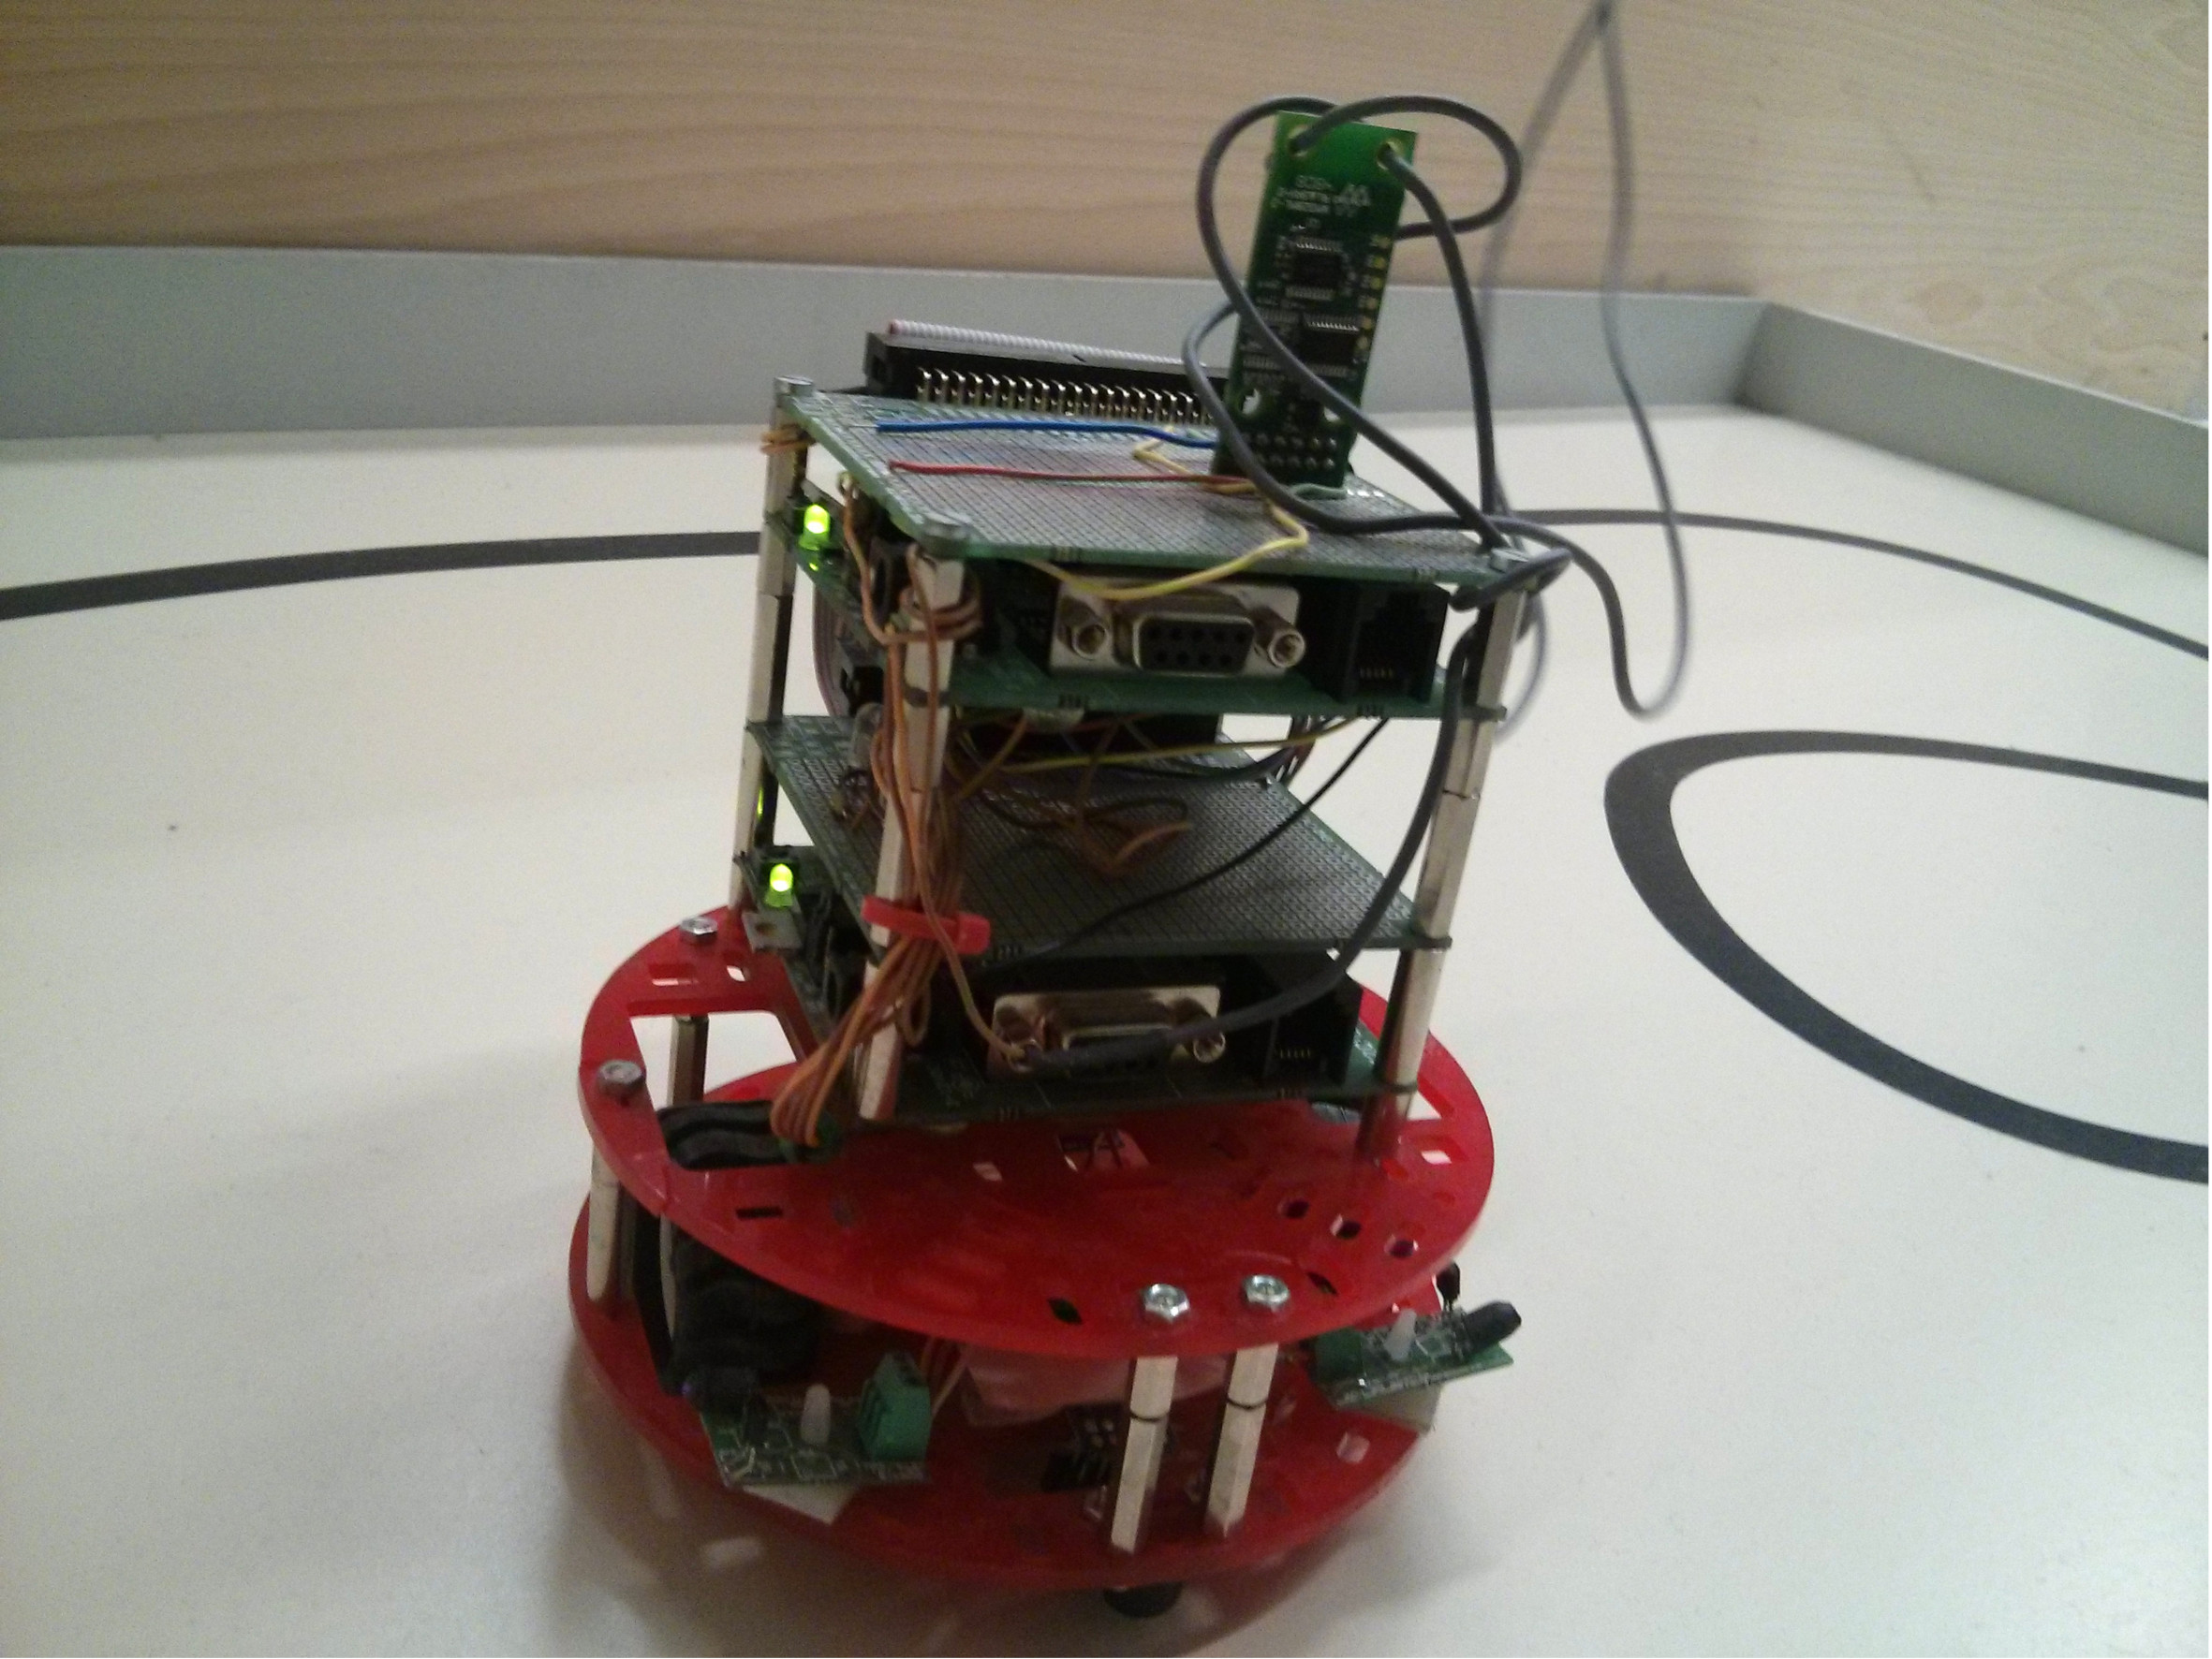
\includegraphics[width=0.5\textwidth]{fig/weblab-bot}
	\caption{WebLab-Bot, a robot based on Azkar-Bot. A remote laboratory in WebLab-Deusto.}
	\label{fig:weblab-bot}
\end{figure}

Moreover, in \acrlong{tli} (\acrshort{tli}), they have a robot called iRobot, that teaches how to
deal with accuracy of sensors, localization and mapping. Finally, the robot that will be used in
this project is called Romie (Figure~\ref{subfig:romie}). It is located in WebLab-Deusto and it has
the needed functionality for this project: it is capable of following a line, it detects walls and
it detects intersections. WebLab-Deusto has a complete labyrinth for it where we will deploy this
project (figure~\ref{subfig:labyrinth}).

\begin{figure}[ht]
	\centering
	\begin{subfigure}{0.35\textwidth}
		\centering
		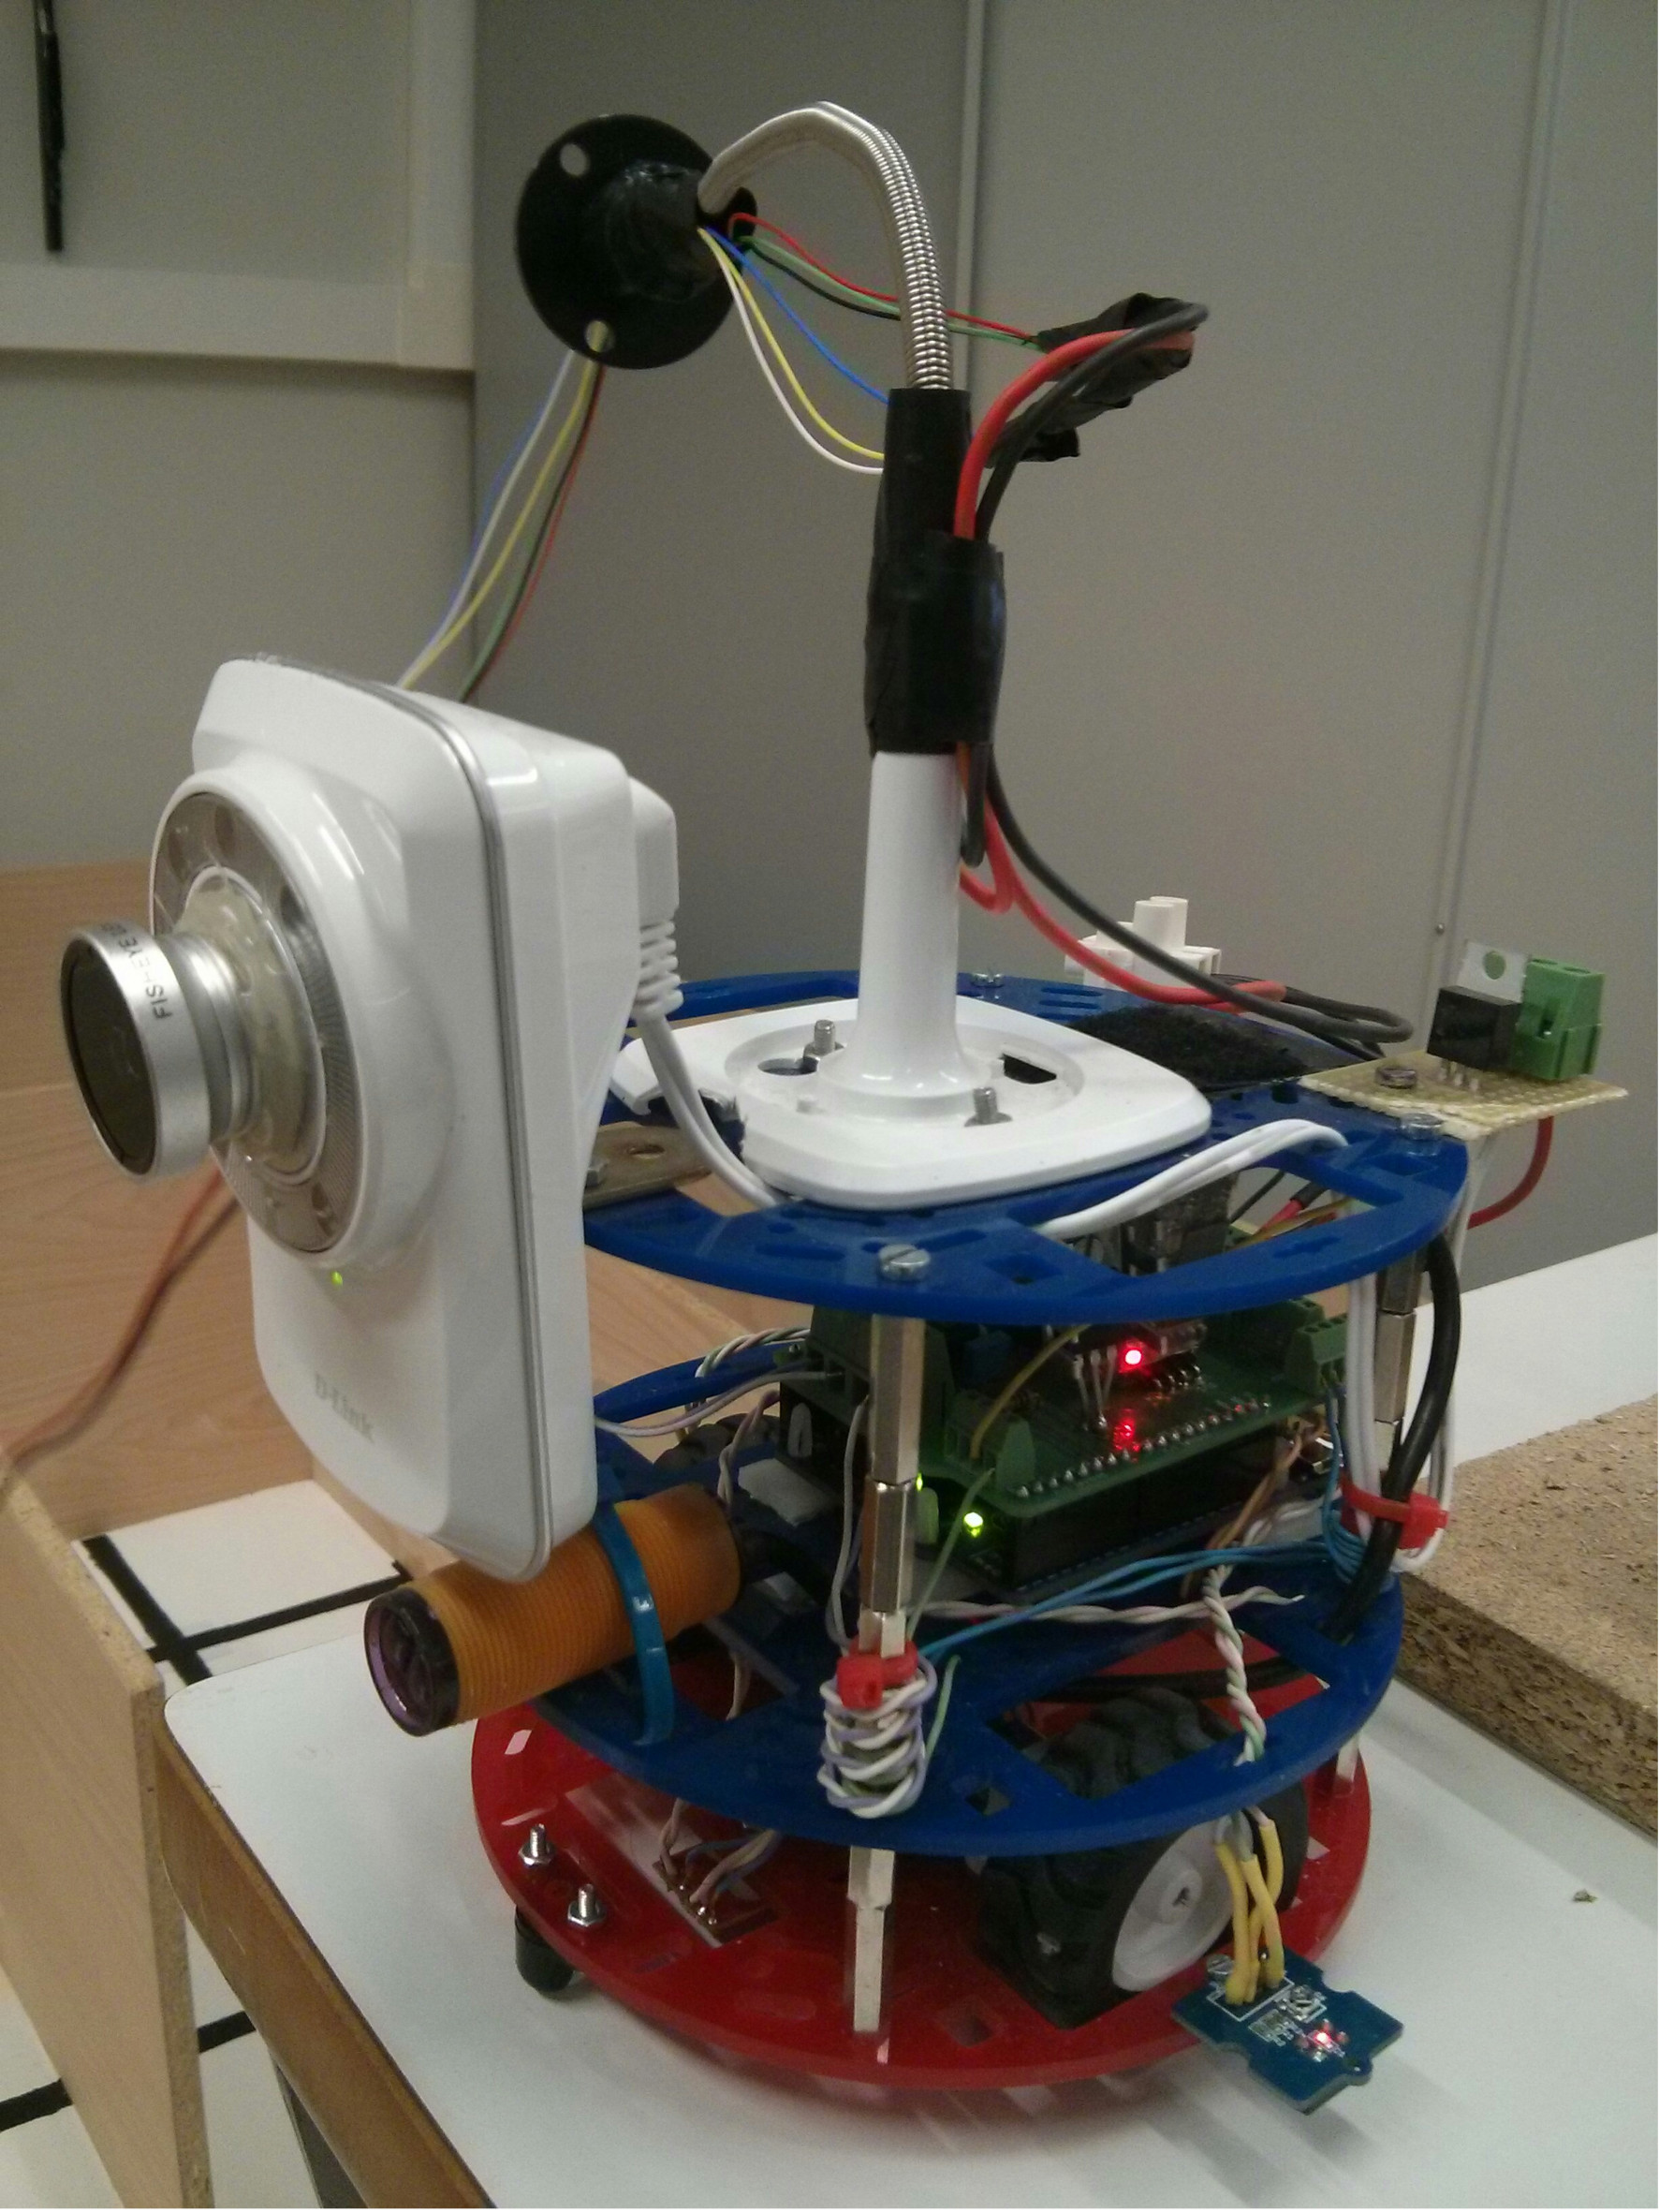
\includegraphics[width=0.8\textwidth]{fig/romie}
		\caption{Romie, the robot.}\label{subfig:romie}
	\end{subfigure}\quad
	\begin{subfigure}{0.55\textwidth}
		\centering
		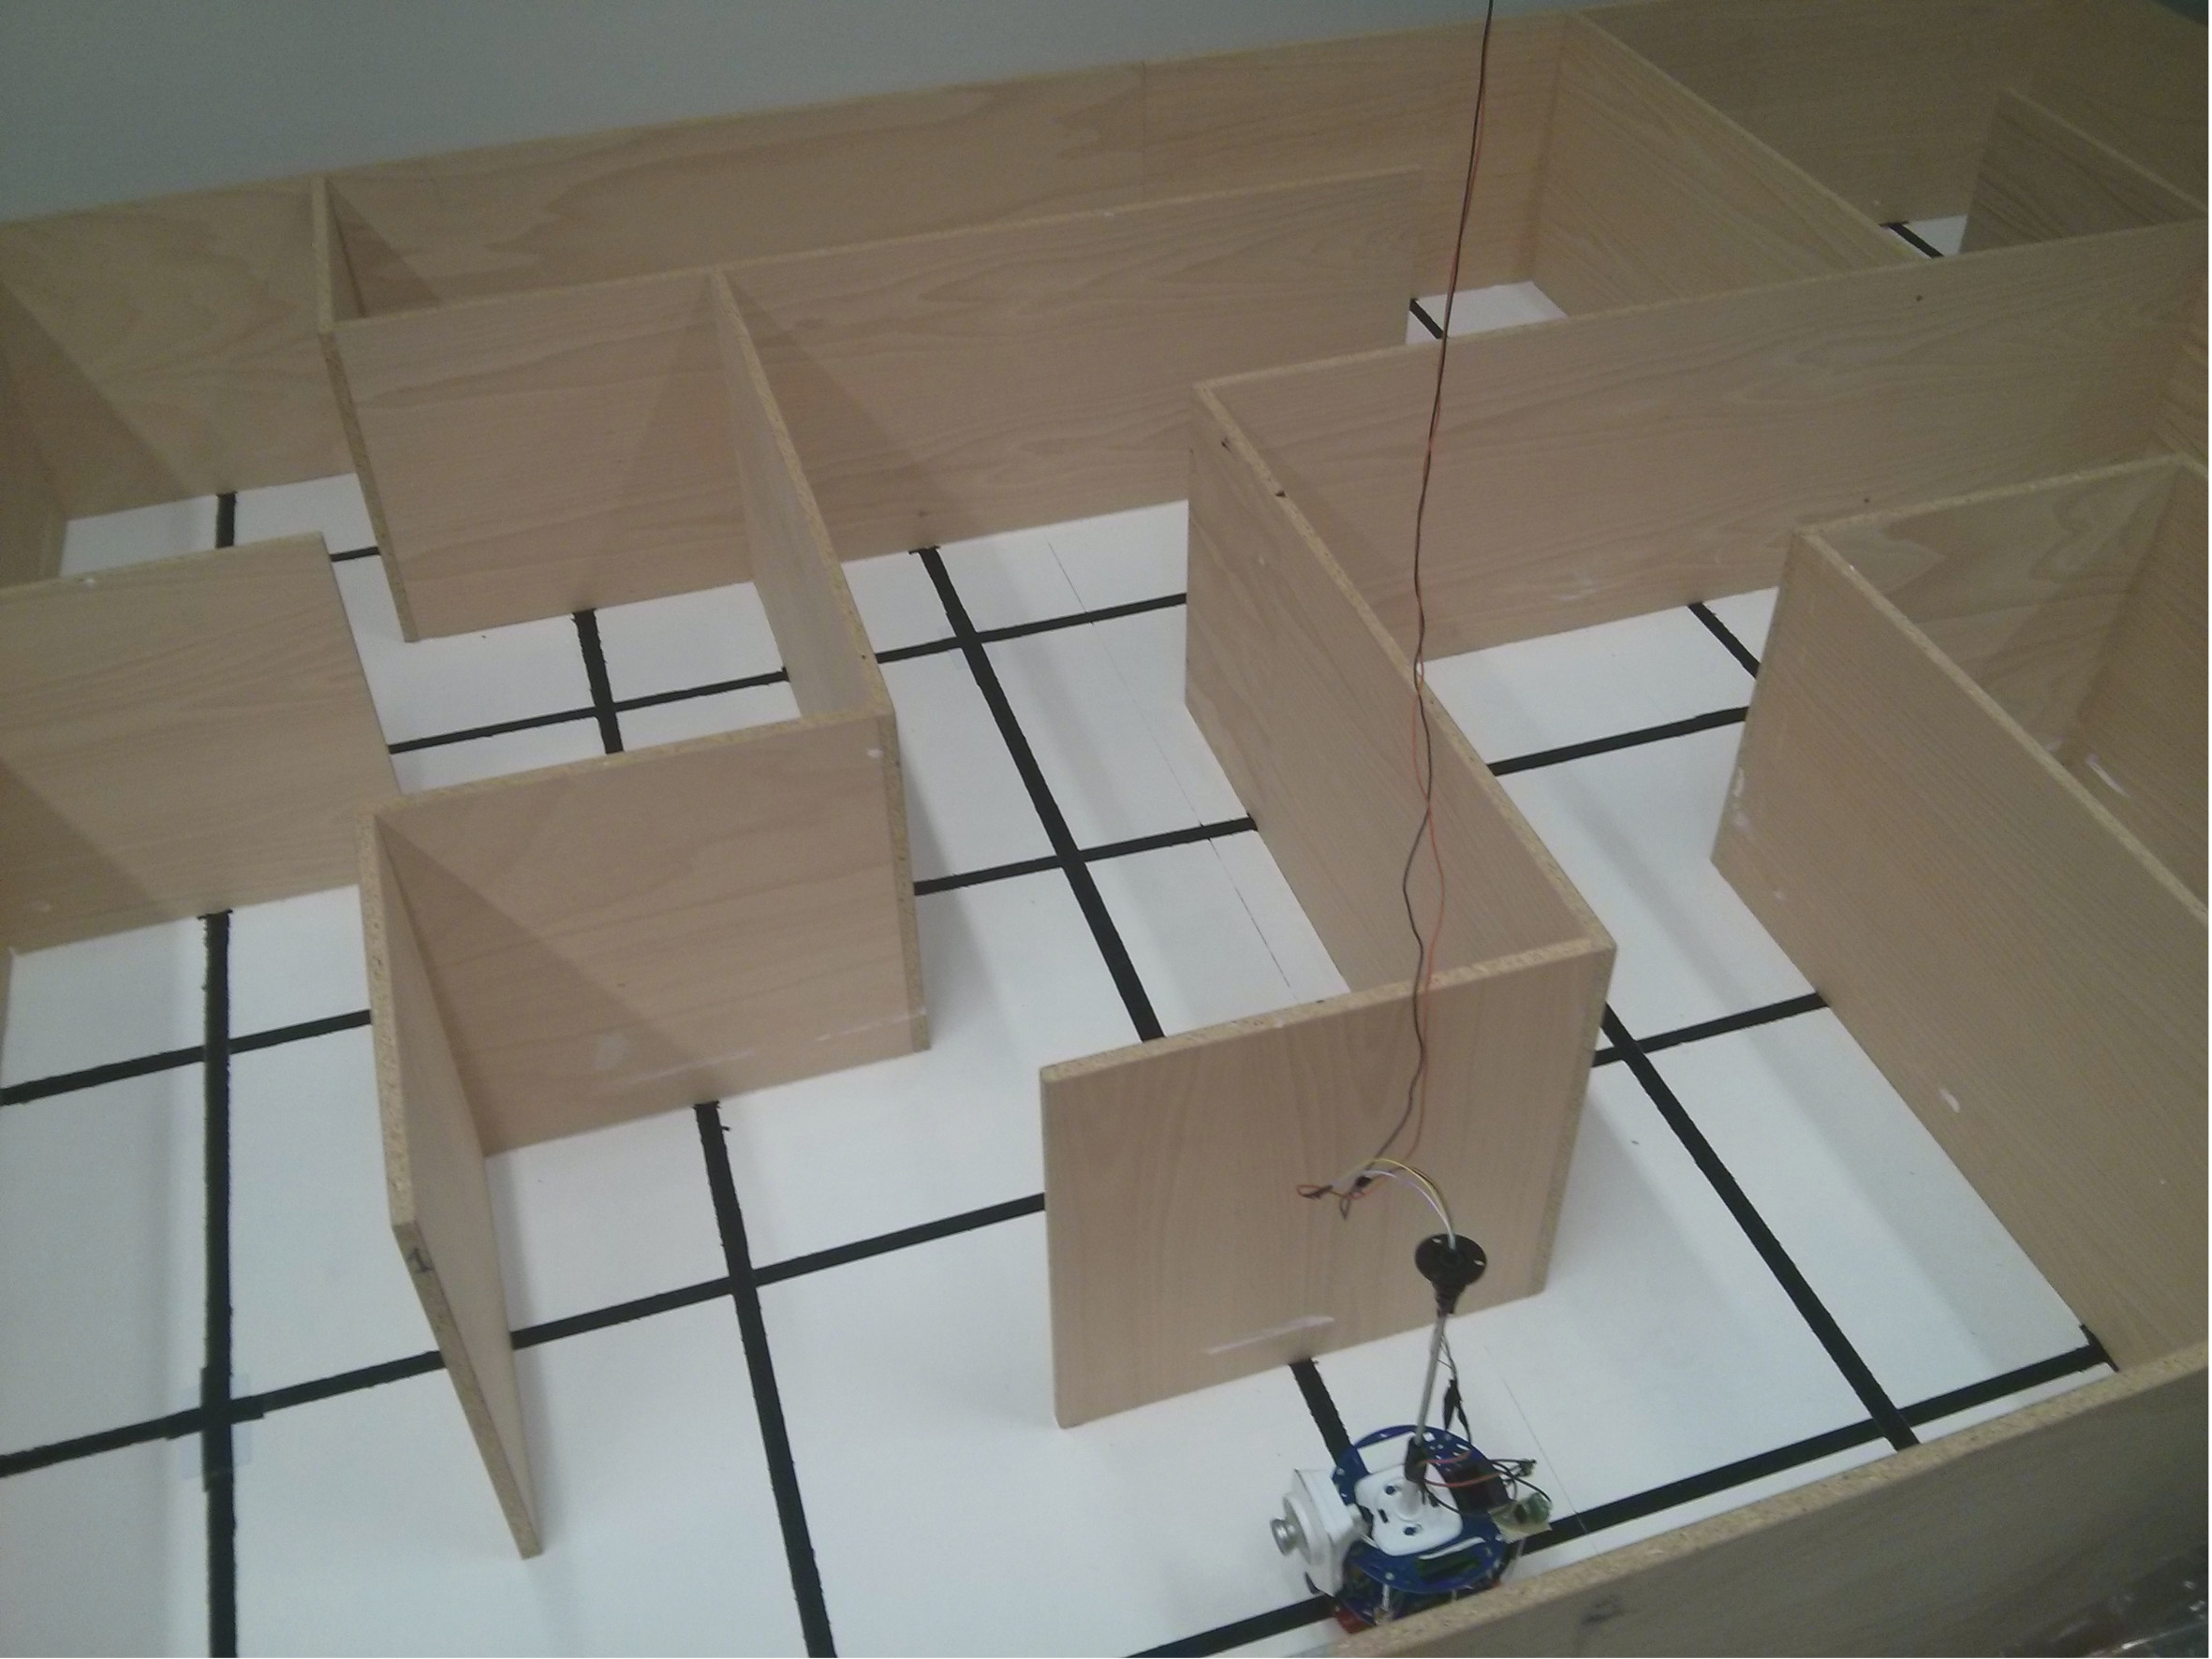
\includegraphics[width=0.8\textwidth]{fig/labyrinth}
		\caption{The labyrinth where Romie will have to move.}\label{subfig:labyrinth}
	\end{subfigure}\quad
	\caption{The robot that will be used in this project.}
\end{figure}

\subsubsection{Simulations}

Even if the project will not be based on simulated robotics but in real robots, currently some
projects use simulations to bring some of the experience to users. A simulation is usually less
costly than a remote laboratory, since not much specialized hardware is required. On the other hand,
students will not be using real tools and experimentation environments, so the experience of using
them will not be as complete as in a remote laboratory.

Nevertheless, some prefer creating hybrid laboratories~\cite{hybrid_labs}. In these cases, the
laboratories add a simulation layer over the real laboratory. This way, the user still uses a real
laboratory, with the benefits of knowing how to use the laboratory and doing real experimentation,
and it also gives the user some more benefit by simulating extra conditions that could be expensive
to create in a real laboratory.

\subsection{Serious Games and Visual Programming}

Serious games are video games that do not only entertain, but they manage to teach. Thanks to that,
they can be used to improve the quality of the learning environment for students. Moreover, since
games in many cases attract better the attention of young people, they can even be a better tool for
teaching, at least, the basic concepts of some subjects~\cite{serious_games}.

We will check some serious games, and we will also analyze the most known tools for visual
programming environments, since we will use these tools for creating one of our scenarios.

TODO: analyze serious games

Visual programming is a way of programming that instead of using real code in a real programming
language uses a visual interface to create programs and then translate them to a well known
language. This way, people that are not yet used to programming languages, interfaces such as
\acrshort{ide}s (\acrlong{ide}s) or code execution, and do not understand the basis of programming
can start learning by using a simple visual environment~\cite{visual_programming}.

\subsubsection{Scratch}

Scratch is one of the most known visual programming tools~\cite{scratch}. It is in itself an
\acrshort{ide}, made by the \acrshort{mit} to help to teach programming to inexperienced users. It
teaches the basic concepts of algorithms and it gives an enough powerful tool so that users can
enjoy using it. It's main concept is to join basic programming blocks so that functionality is
created.

Moreover, they have created a complete collaboration platform where all the users of Scratch can
share their creations and check out the ones that others have made. That way, users can learn more
by looking at code created by others.

\subsubsection{Blockly}

Blockly, unlike Scratch, is not a visual programming \acrshort{ide}, but a visual programming
library to create visual programming editors and \acrshort{ide}s. It has the same basis as Scratch,
so it contains basic programming blocks to build applications by joining them
(Figure~\ref{fig:blockly}), and it also gives developers the option to create their own blocks with
a simple \acrlong{api} or \acrshort{api}. It was created by Google and it's source is now available
in GitHub~\cite{blockly}.

\begin{figure}[ht]
	\centering
	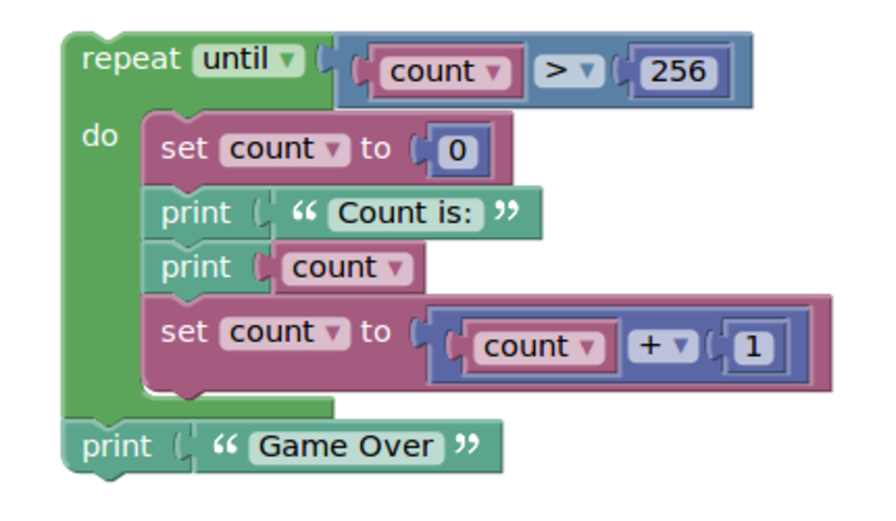
\includegraphics[width=0.5\textwidth]{fig/blockly}
	\caption{Simple program example created in Google's Blockly.}\label{fig:blockly}
\end{figure}

Blockly enables developers to create their own programming environments for their projects, so they
can adapt Blockly itself to their needs, and thus, making it possible for them to even create
complete \acrshort{ide}s for their projects based on visual programming.

\subsection{WebLab-Deusto}

WebLab-Deusto is a remote laboratory facility located in the University of Deusto, Bilbao. Since
2001, it has been providing students with remote laboratories to complete their academic
learnings~\cite{weblab}. Since then, it has been extended and many of it's laboratories is available
all over the world. It's no longer a laboratory only made for microelectronics university students
since nowadays it serves schools and universities everywhere to provide them with remote
laboratories.

Among others, it serves an experiment to prove and measure the Archimedes' principle
(Figure~\ref{fig:archimedes}), an experiment to program and control a robot and some
microelectronics experiments with \acrlong{pld}s or \acrshort{pld}s and \acrlong{fpga}s or
\acrshort{fpga}s. Moreover, there are more laboratories in development, such as an elevator to teach
students how to program and control them, an experiment with an aquarium where students can give
them food and, of course, the project presented here: a complete learning and gaming experience
brought remotely using a robot, Romie.

\begin{figure}[!htbp]
	\centering
	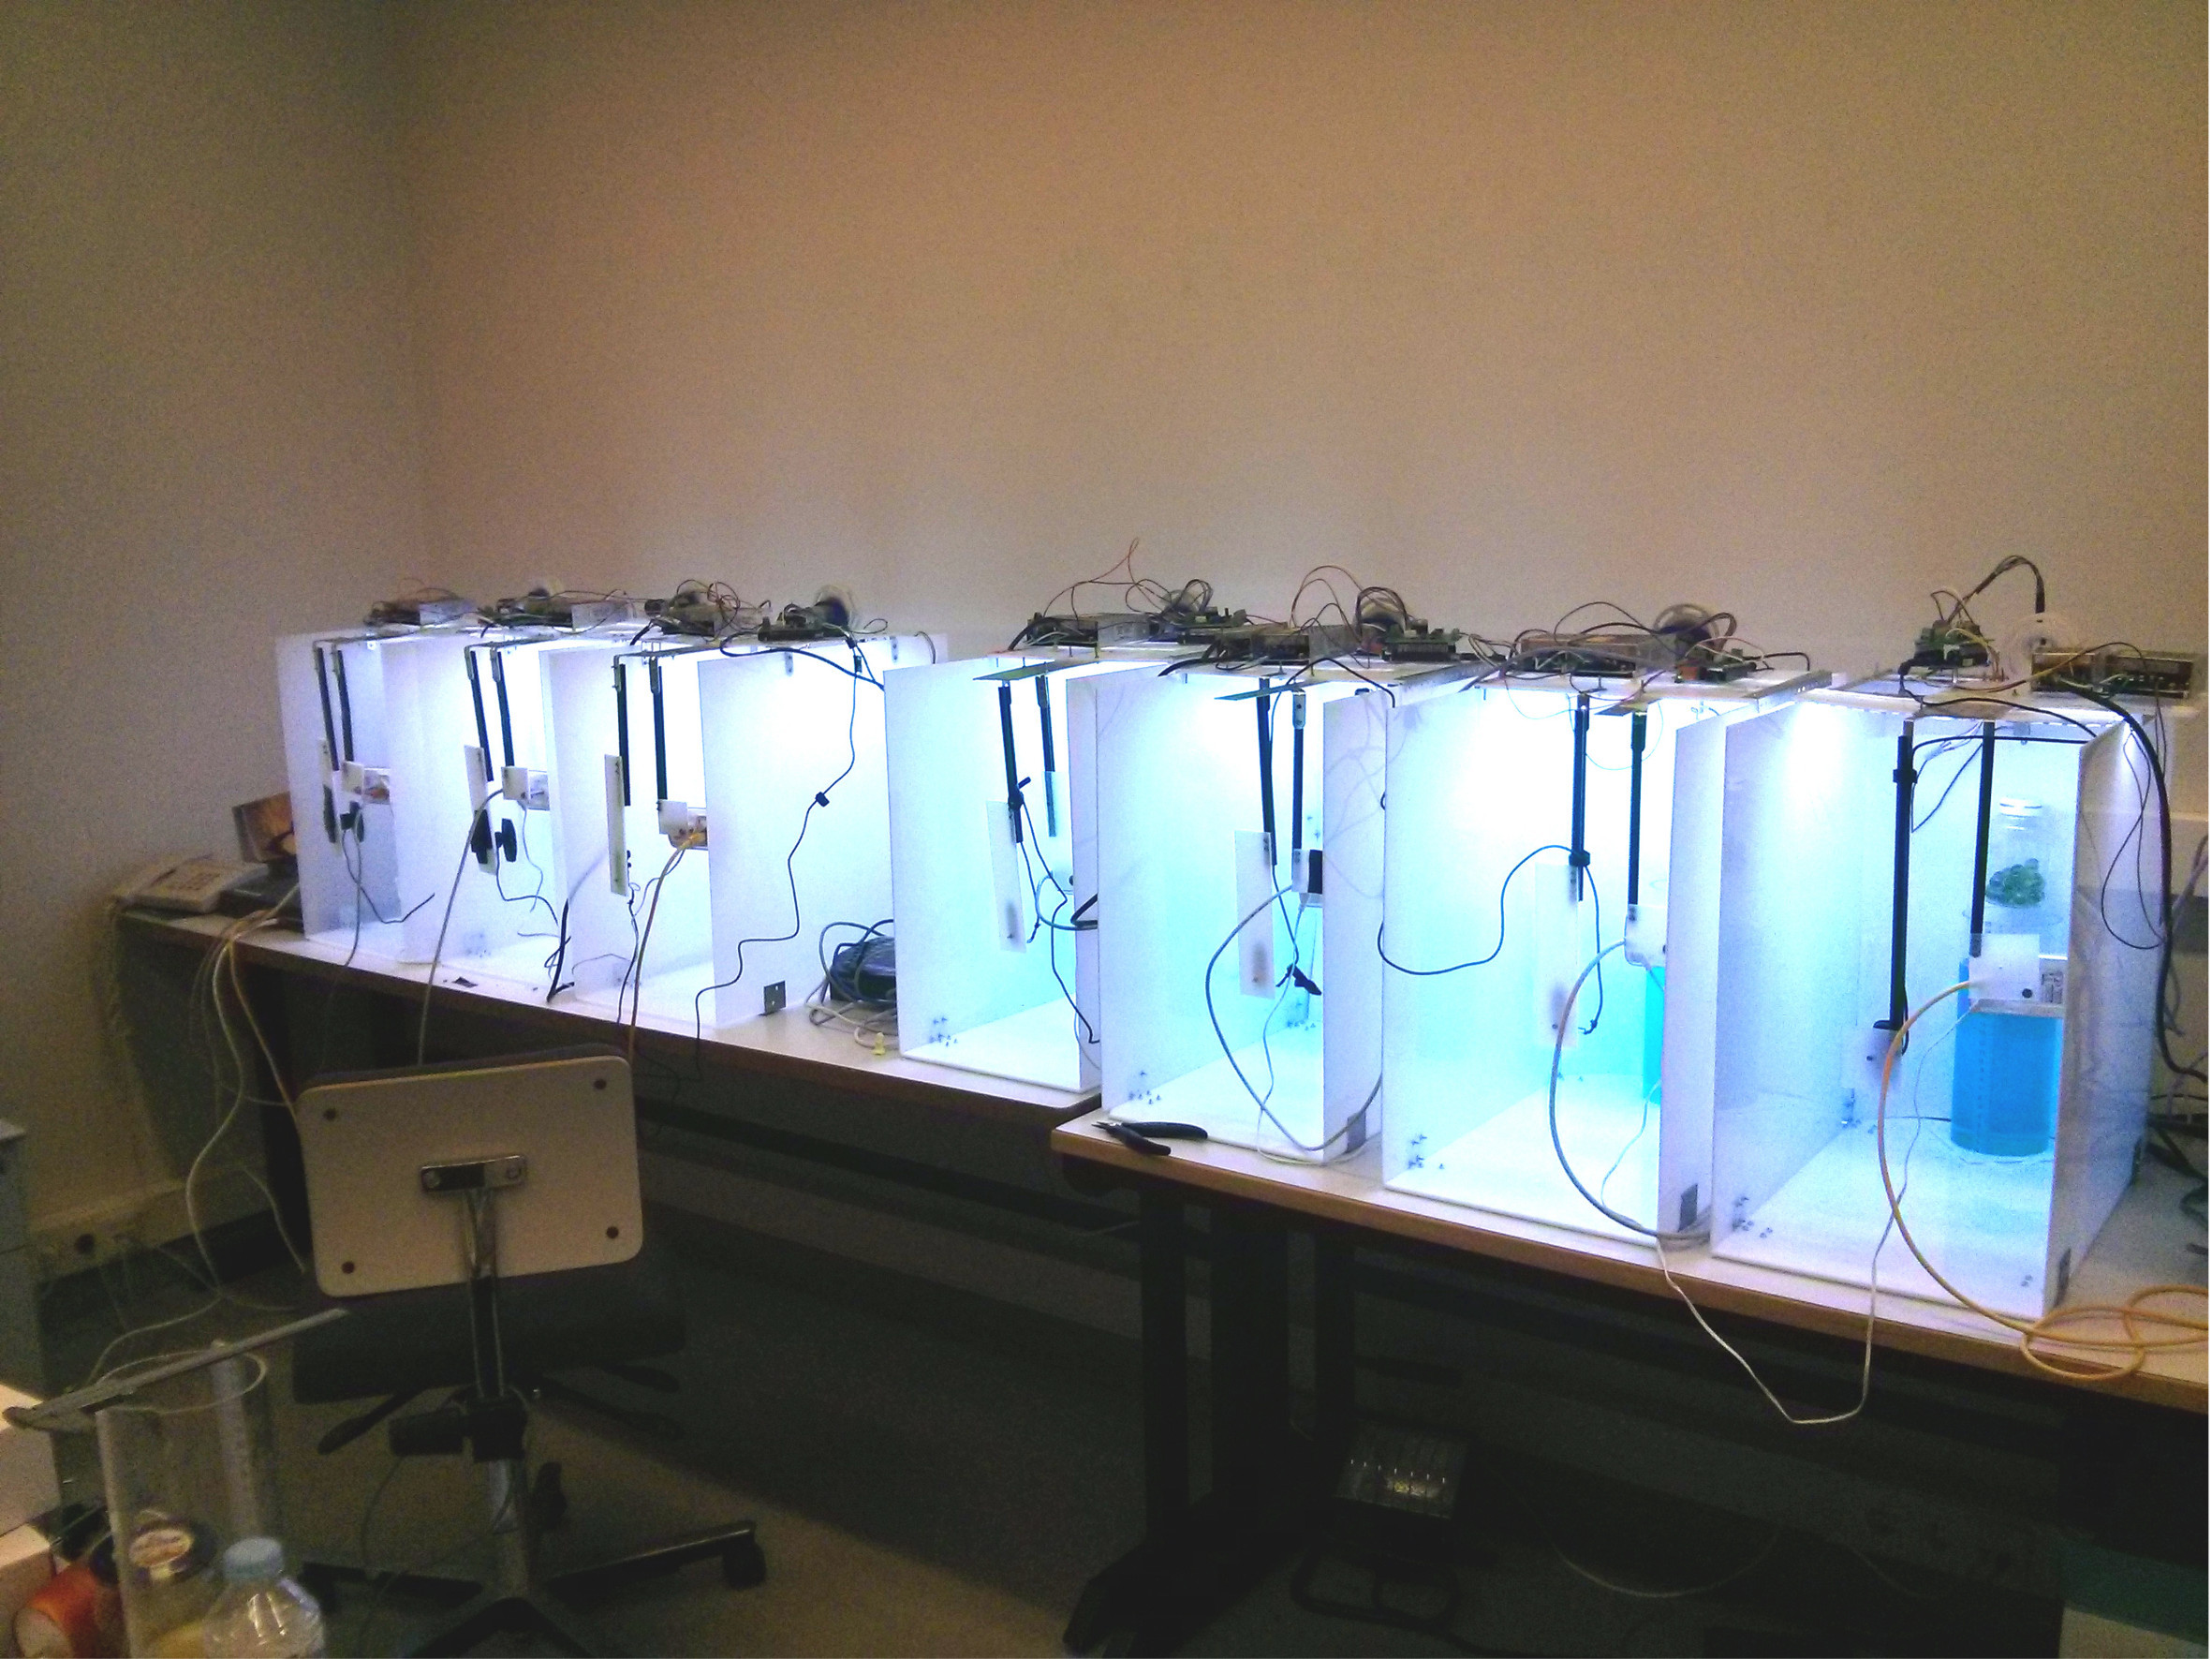
\includegraphics[width=0.5\textwidth]{fig/archimedes}
	\caption{Archimedes experiment in WebLab-Deusto.}\label{fig:archimedes}
\end{figure}

\section{Rationale}

Remote laboratories are a platform developed to reduce costs of experimentation for schools by
moving the laboratories themselves to the cloud. Nevertheless, this is only one of the multiple uses
a platform like this can have, and in this project, the challenge is to demonstrate how remote
laboratories can be used for serious gaming.

This project will be at the best of our knowledge the first game platform based on remote
laboratories, it will open the course to future developments in this area by enabling future games
to be developed using this technology.

It will be a challenge to adapt the current technology and experimentation platforms to this kind of
project, but the result can be unique and powerful for teaching all kind of knowledge in a fun way
by using real gamification processes in a remote laboratory platform.

\chapter{Goals and Scope}

The platform will integrate sophisticate hardware and software elements that allow us to deploy a
remote controlled robot so that it can be used by students in a game platform using the provided
user interface.

The development of the project will require knowledge about the hardware (for the maintenance and
modifications of the robot), knowledge about communication protocols (\acrlong{http} or
\acrshort{http}, \acrshort{tcp}/\acrshort{ip} and Bluetooth) for command and image transmission,
knowledge about web engineering (for the development of the client and the interaction with the
WebLab-Deusto platform) and user interface design knowledge for creating a user-friendly interface
taking into account the requirements asked by the ``\acrlong{fecyt}'' (\acrshort{fecyt}) ``Ciencia
remota'' initiative.

\section{Project Definition}

The secondary objectives of the project will be the following:
\begin{itemize}
\item \textbf{Requirement analysis, state of the art study. Requirements specification}:

A complete state of the art study will be performed to know th current market situation regarding to
remote robotic laboratories and the \acrshort{stem} promotion in young people. Moreover, a
requirement analysis will be performed which will give us the final requirement specification.

\item \textbf{\acrshort{stem} element revision for young students}:

We will analyze which are the most influential elements in the education of students in the
\acrshort{stem} area so that they can be maximized when developing the platform. They will be proved
with young students aged between 10 and 18 years old.

\item \textbf{Current hardware platform analysis and modification}:

We will study the possibilities of the current hardware in WebLab-Deusto (the robot Romie) and the
needed changes will be developed to adapt it to the needs of the project.

\item \textbf{\acrshort{api} for remote control}):

A complete control \acrshort{api} will be developed, able of communicating with the robot with a
a simple interface for the client software taking into account the restrictions of the WebLab-Deusto
environment.

\item \textbf{Trivial type game platform development - registration, game design, score and robot
control}:

A game platform will be created based on a simple trivial type game, where the user will have to
answer the proposed questions to obtain a high score. A contest will take place where these users
will get a prize. Game rules must be carefully analyzed so that the game will not be too easy nor
too difficult.

\item \textbf{Integration of a psychological experiment for fighting against pseudoscience working
with a psychologist group}:

The psychology laboratory of the University of Deusto, Labpsico will provide an experiment about the
fight against pseudoscience that will be added to the game in one of its game modes. The relevant
data for the psychological research will be sent to Labpsico, while the user will receive a bonus in
the game depending on his or her performance in the psychological activity.

\item \textbf{Visual programming environment for the robot}:

A visual programming environment for the robot will be created based on one of the most known
platforms: Blockly or Scratch, still to be decided, depending on the previous research. This
environment will be used to teach the basics of programming to young students.

\item \textbf{Integration in WebLab-Deusto}:

We will use the WebLab-Deusto platform provided by the University of Deusto so that we can deploy
the experiment in a production environment along with the rest of the experiments. This provides the
experiment with a simple interface for the communication with the experiment server and with the
robot. It will also be in charge of managing user queues and user authentication.

\item \textbf{Platform dissemination: Deployment in the ``Ciencia Remota'' project of
\acrshort{fecyt} and testing by students}:

The game will be deployed in th ``Ciencia Remota'' projct of \acrshort{fecyt} where many
institutions work to bring remote experimentation to more places. For that, and as a demonstration
of the potential of the project, some public test will be performed where students from various
schools will take part.

\item \textbf{Usage statistics report}:

A complete report will be generated to learn from the use statistics. This will provide us with
information on how to improve the game.

\end{itemize}

\section{Description of the Embodiment}

\subsection{Development Methodology}

\begin{figure}
	\centering
	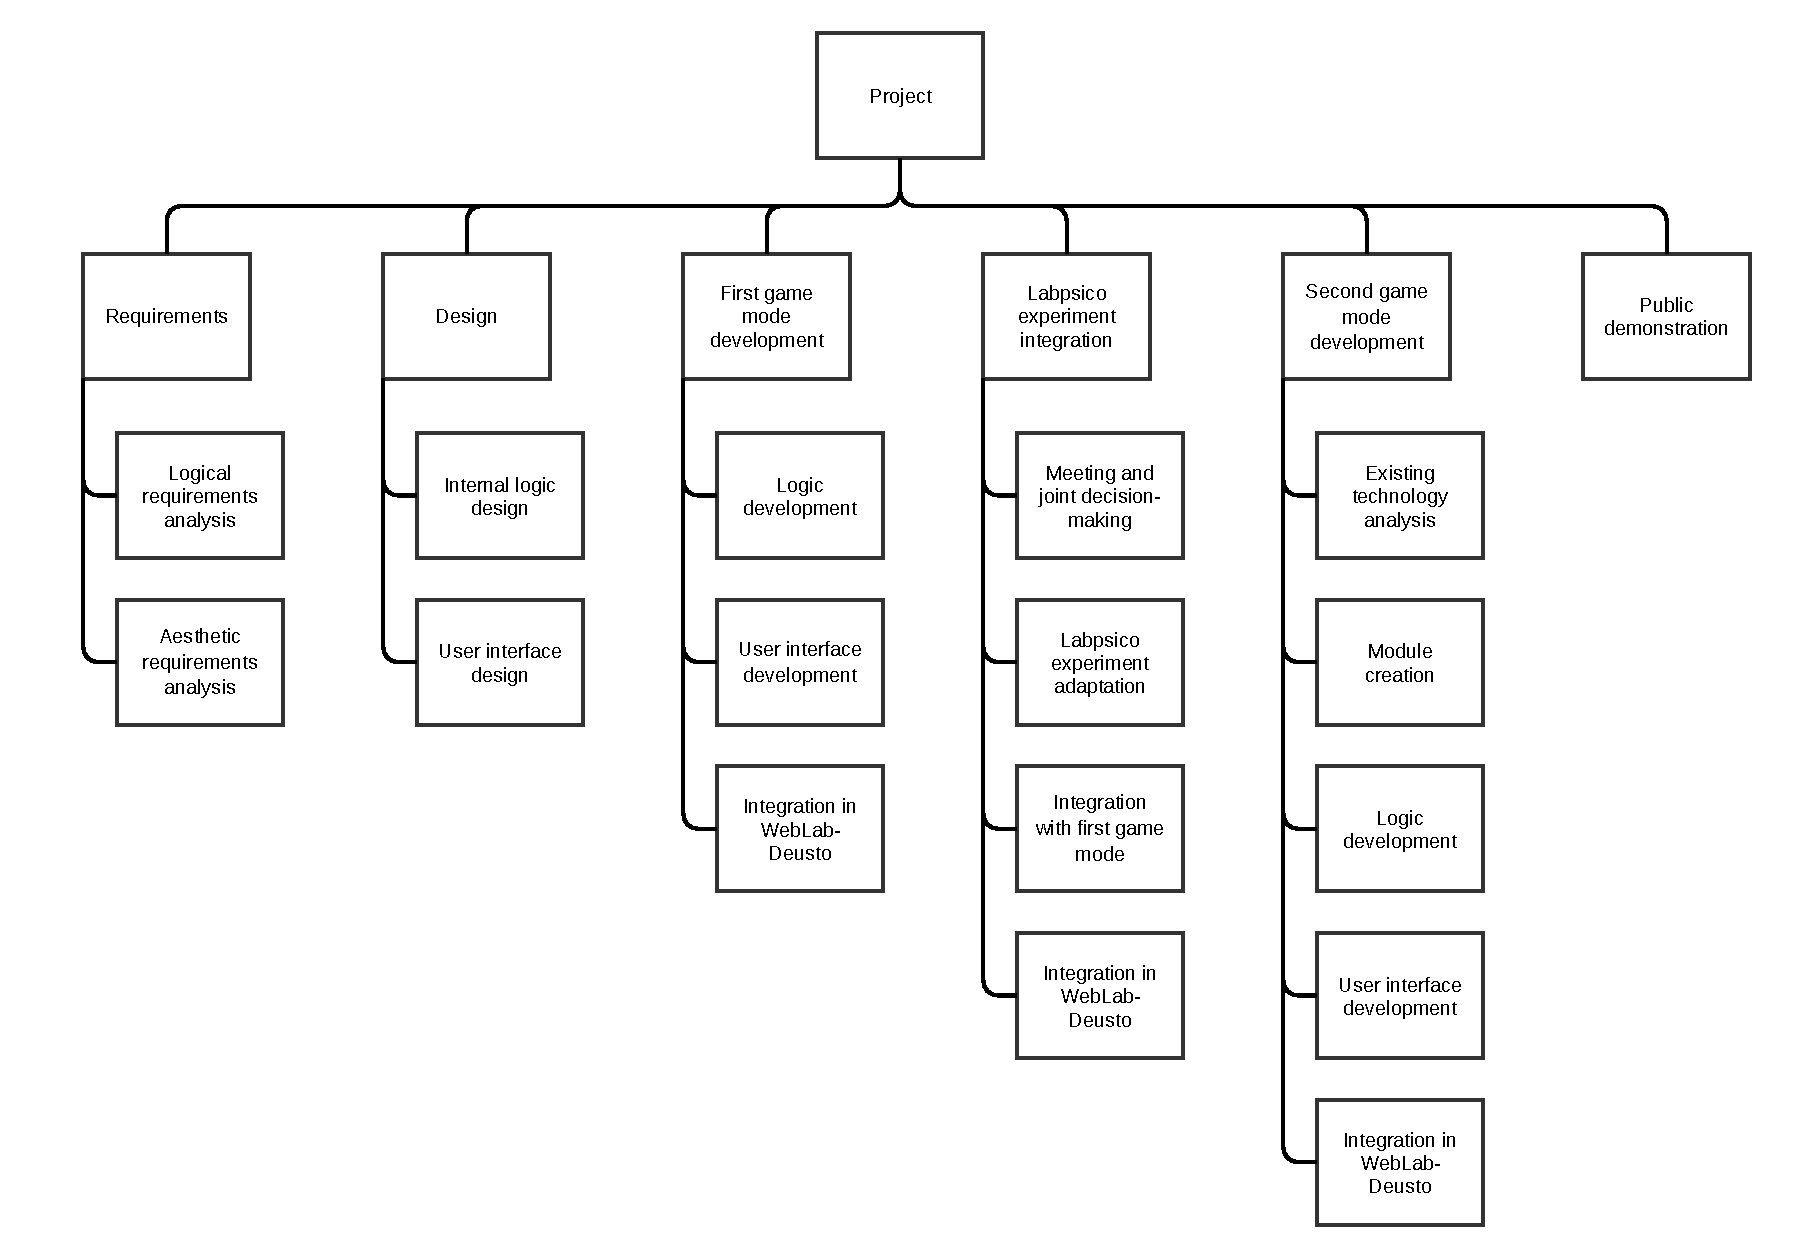
\includegraphics[height=0.9\textwidth, angle=90]{fig/wbs}
	\caption{Project's \acrlong{wbs}.}\label{fig:wbs}
\end{figure}

In the project's \acrlong{wbs} or \acrshort{wbs} (figure~\ref{fig:wbs}) we can see how the project
will be developed, and how the task will be divided. As we can see in the \acrshort{wbs}, the phases
of the project will be the following:

\begin{itemize}
\item \textbf{Requirements}: Project's requirements analysis, in which functional and aesthetic
requirements will be determined.

\item \textbf{Design}: Comprehensive design of the project, both functional and aesthetic, to define
the final product.

\item \textbf{First game mode development}: The first intermediate product will be developed, and it
will be integrated in the WebLab-Deusto platform. This game will be a trivial type game.

\item \textbf{Labpsico experiment integration}: An experiment provided by the University of Deusto's
psychology laboratory, Labpsico, will be integrated with the first game mode.

\item \textbf{Second game mode development}: The second game mode will be developed, based on visual
programming, to teach computing logic.

\item \textbf{Public demonstration}: A public demonstration will be performed to test the viability
and reliability of the project with students.
\end{itemize}

\subsection{Intermediate Products}

These will be the intermediate products that the project will produce:

\begin{itemize}
\item \textbf{First game mode}: This game mode will be a trivial type game, where the user will move
the robot in a labyrinth and will have to replay questions in specific location.

\item \textbf{First game mode with Labpsico experiment}: The same game mode as the one before will
be modified to accommodate the experiment provided by Labpsico, based on a psicology experiment
to fight against pseudoscience.

\item \textbf{Second game mode}: A second game mode will be created where users will be able to
program actions to the robot and make it move around the labyrinth.
\end{itemize}

\subsection{Main Tasks}

\subsubsection{Requirements}

\begin{itemize}
\item \textbf{T1 - Logical requirements analysis}: A detailed analysis will be performed to
understand all the functional requirements of the platform. That way we will be able to track them
and check its fulfillment.

\item \textbf{T2 - Aesthetic requirements analysis}: A detailed analysis will be performed to
understand all the aesthetic requirements of the platform. That way we will be able to track them
and check its fulfillment.
\end{itemize}

\subsubsection{Design}

\begin{itemize}
\item \textbf{T3 - Internal logic design}: The internal logic of the robot and the control platform
have to be designed in thinking on accessibility, stability and simplicity.

\item \textbf{T4 - User interface design}: The \acrlong{ui} of the platform has to be designed
thinking on the final user, so that the robot is easy to control.
\end{itemize}

\subsubsection{First game mode development}

\begin{itemize}
\item \textbf{T5 - Logic development}: The internal logic of the trivial type game will be developed
thinking always on the modularity and extensibility.

\item \textbf{T6 - User interface development}: A \acrlong{ui} will be developed taking into account
usability standards to use the robot and answer questions.

\item \textbf{T7 - Integration in WebLab-Deusto}: The game platform will be integrated in
WebLab-Deusto using its queue and priority management systems.
\end{itemize}

\subsubsection{Labpsico experiment integration}

\begin{itemize}
\item \textbf{T8 - Meeting and joint decision making}: We will have a meeting with the psychology
laboratory of the University of Deusto, Labpsico, where we will decide how to integrate their
experiment with the first game mode.

\item \textbf{T9 - Labpsico experiment adaptation}: The experiment provided by Labpsico will be
adapted to make sense in the experiment with the robot.

\item \textbf{T10 - Integration with first game mode}: The experiment will be integrated with the
existing platform with the robot using the interface created for the first game mode.

\item \textbf{T11 - Integration in WebLab-Deusto}: The new game will be integrated in WebLab-Deusto
using its queue and priority management systems.
\end{itemize}

\subsubsection{Second game mode development}

\begin{itemize}
\item \textbf{T12 - Existing technology analysis}: A detailed analysis will be performed to decide
which visual programming tool will be the one used for this game mode.

\item \textbf{T13 - Module creation}: The modules needed for controlling the robot will be created.

\item \textbf{T14 - Logic development}: The game logic will be developed so that the program created
by the user can control the robot.

\item \textbf{T15 - User interface development}: A simple \acrlong{ui} will be developed to be able
to use all the functions of the visual programming mode.

\item \textbf{T16 - Integration in WebLab-Deusto}: The visual programming environment will be
integrated in WebLab-Deusto using its queue and priority management systems.
\end{itemize}

\subsubsection{Public demonstration}

\begin{itemize}
\item \textbf{T17 - Public demonstration}: At least one public demonstration of the robot will be
performed during its development where students will try it and play with it.
\end{itemize}

\section{Organization}

\subsection{Organizational Structure}

The working team, as it can be seen in the figure~\ref{fig:org}, it will be organized in a direction
committee, that will be in charge of the good progress of the project, as well as of indicating
the possible needed changes, and in a development team, that will be in charge of developing the
project. Moreover, in the integration of the Labpsico experiment, the Labpsico team will be part of
the project organization team to validate the progress.

\begin{figure}[ht]
	\centering
	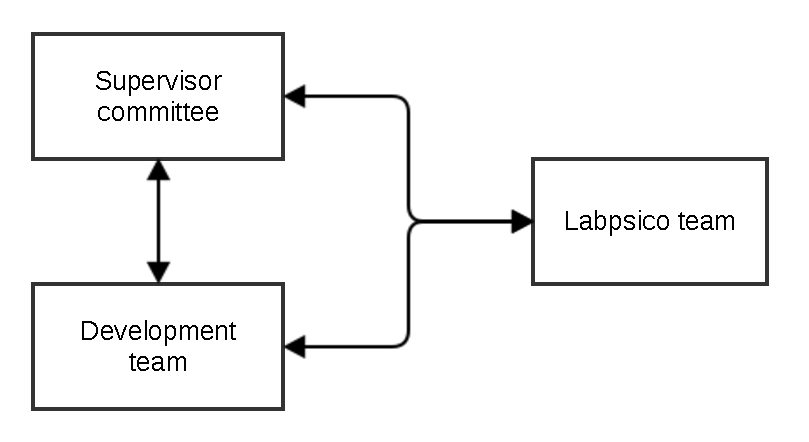
\includegraphics[width=0.7\textwidth]{fig/organization}
	\caption{Project's organization schema.}\label{fig:org}
\end{figure}

\subsection{Human Resources Plan}

The workday will be part time, 4 hours and we will only have one resource, that will be divided into
the following profiles:

\begin{itemize}
\item One \textbf{project manager}: he will be the person in charge of organizing the project.

\item One \textbf{programmer}: he will be the person in charge of developing the logic of the
software.

\item One \textbf{designer}: he will be the person in charge of designing and creating a
\acrlong{ui} intuitive and simple.

\item One \textbf{WebLab-Deusto expert}: he will be in charge of the integration of the experiment
in WebLab-Deusto.
\end{itemize}

Regular meetings will be done, at least twice a month to track the project progress. To validate the
various modules of the application, we will check if the established requirements are met, and
volunteers of the team will perform the needed testing. The organization of the working team will
not be hierarchical but rather horizontal, to allow a much more agile development.

\chapter{Planning}

In the table~\ref{tab:plan} the planning for the project can be observed. The workloads can be seen
in the table~\ref{tab:work}. It has been decided to do Task 3 and Task 4 in parallel even if that
supposes to divide the working day in two tasks, since having only one resource and being part of
the development of the same intermediate product, both tasks could benefit from the parallel
development. The same decision has been made with tasks T14 and T15 for the same reasons.

\begin{table}[h]
	\centering
	\caption{Project planning.}\label{tab:plan}
	\begin{tabular}{ccccccc}
		\toprule
		\textbf{Task} & \emph{Dep.} & \emph{Resource} & \emph{Days} & \emph{Work} & \emph{Start date} & \emph{Ending date}\\
		\midrule
		T1	&				& Project Manager		& 1 day		&	2 hours		& 01/07/2015	& 01/07/2015	\\
		T2	&				& Project Manager		& 1 day		&	2 hours		& 01/07/2015	& 01/07/2015	\\
		T3	&	T1			& Programmer			& 8 days	&	32 hours	& 01/08/2015	& 01/19/2015	\\
		T4	&	T2			& Designer				& 8 days	&	16 hours	& 01/26/2015	& 02/04/2015	\\
		T5	&	T3			& Programmer			& 18 days	&	56 hours	& 01/20/2015	& 01/16/2015	\\
		T6	&	T4			& Designer				& 7 days	&	28 hours	& 02/17/2015	& 02/25/2015	\\
		T7	&	T5, T6		& WebLab-Deusto	Expert	& 8 days	&	32 hours	& 02/26/2015	& 03/09/2015	\\
		T8	&	T7			& Project Manager		& 1 day		&	2 hours		& 03/13/2015	& 03/13/2015	\\
		T9	&	T8			& Programmer			& 2 days	&	8 hours		& 03/16/2015	& 03/17/2015	\\
		T10	&	T9			& Programmer			& 8 days	&	32 hours	& 03/18/2015	& 03/31/2015	\\
		T11	&	T10			& WebLab-Deusto	Expert	& 4 days	&	16 hours	& 04/13/2015	& 04/16/2015	\\
		T12	&	T11			& Project Manager		& 2 days	&	8 hours		& 04/17/2015	& 04/20/2015	\\
		T13	&	T12			& Programmer			& 5 days	&	20 hours	& 04/21/2015	& 04/27/2015	\\
		T14	&	T13			& Programmer			& 9 days	&	20 hours	& 04/28/2015	& 05/11/2015	\\
		T15	&	T12			& Designer				& 8 days	&	16 hours	& 04/28/2015	& 05/08/2015	\\
		T16	&	T14, T15	& WebLab-Deusto	Expert	& 12 days	&	48 hours	& 05/12/2015	& 05/27/2015	\\
		T17	&	T7			& Project Manager		& 3 days	&	12 hours	& 03/10/2015	& 03/12/2015	\\
		\bottomrule
	\end{tabular}
\end{table}

\begin{table}[h]
	\centering
	\caption{Project workloads.}\label{tab:work}
	\begin{tabular}{cc}
		\toprule
		\textbf{Profile} & \emph{Scheduled hours} \\
		\midrule
		Project Manager			&	26 hours	\\
		Programmer				&	168 hours	\\
		Designer				&	60 hours	\\
		WebLab-Deusto Expert	&	96 hours	\\
		\bottomrule
	\end{tabular}
\end{table}

The Gantt diagram of the project can be seen in figure~\ref{fig:gantt} and the precedence diagram in
figure~\ref{fig:precedence}.

% Gantt diagram in four pages
\begin{figure}
	\centering
	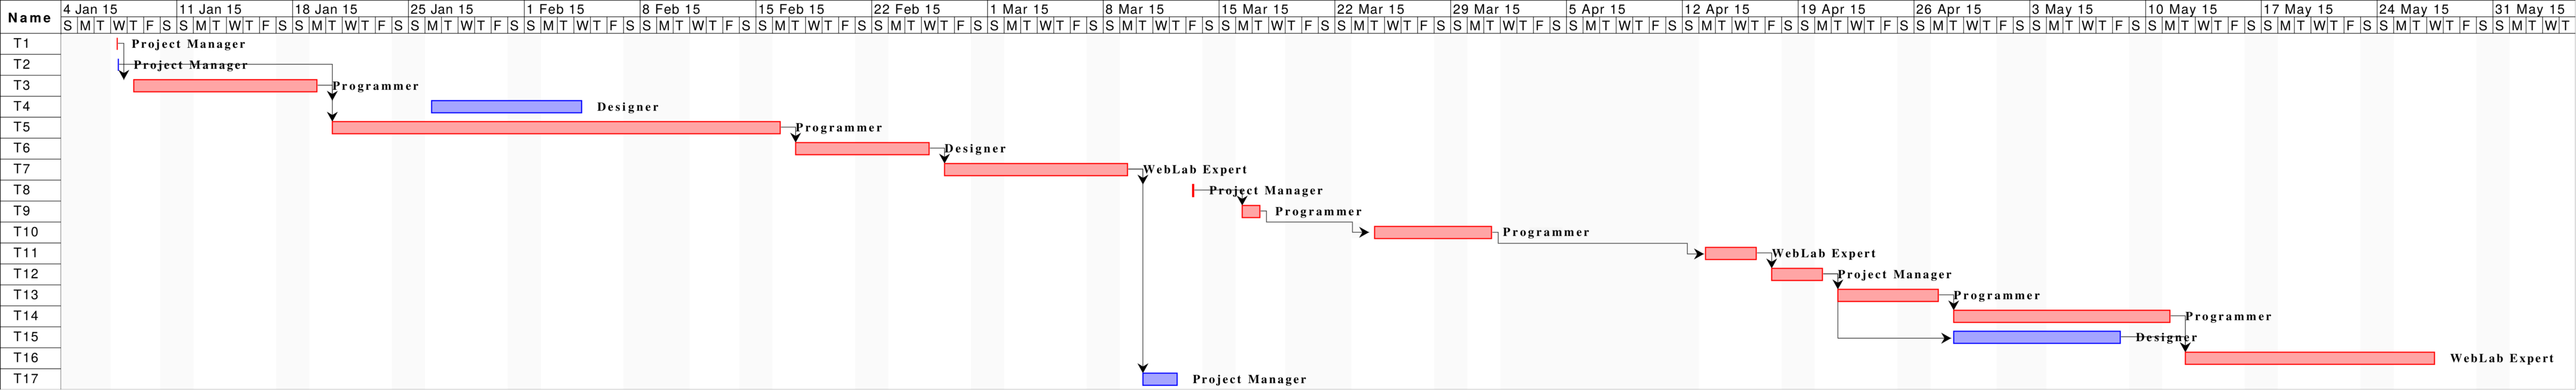
\includegraphics[trim=0in 0in 26in 0in, clip, angle=90]{fig/gantt}
	\caption[Gantt diagram of the project.]{Gantt diagram of the project. Continues in next
	pages.}\label{fig:gantt}
\end{figure}
\clearpage
\begin{center}
	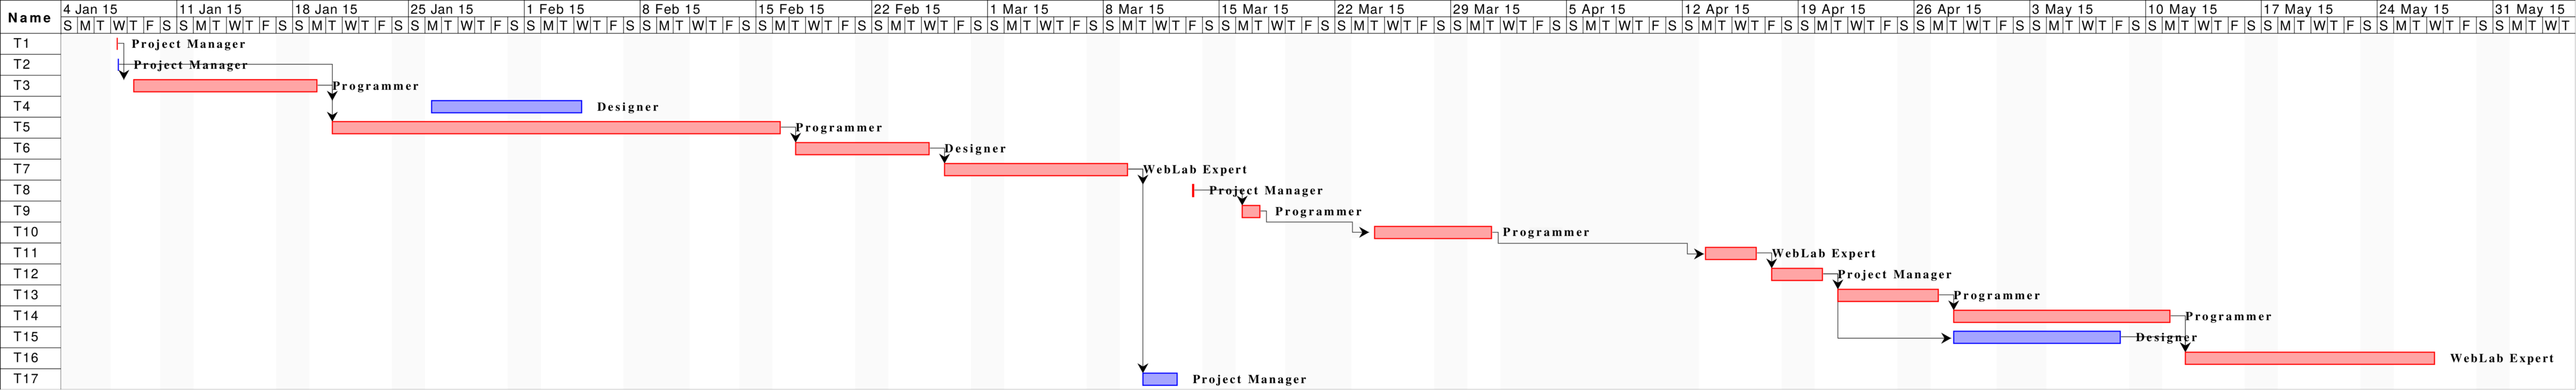
\includegraphics[trim=7.82in 0in 17in 0in, clip, angle=90]{fig/gantt}\clearpage
	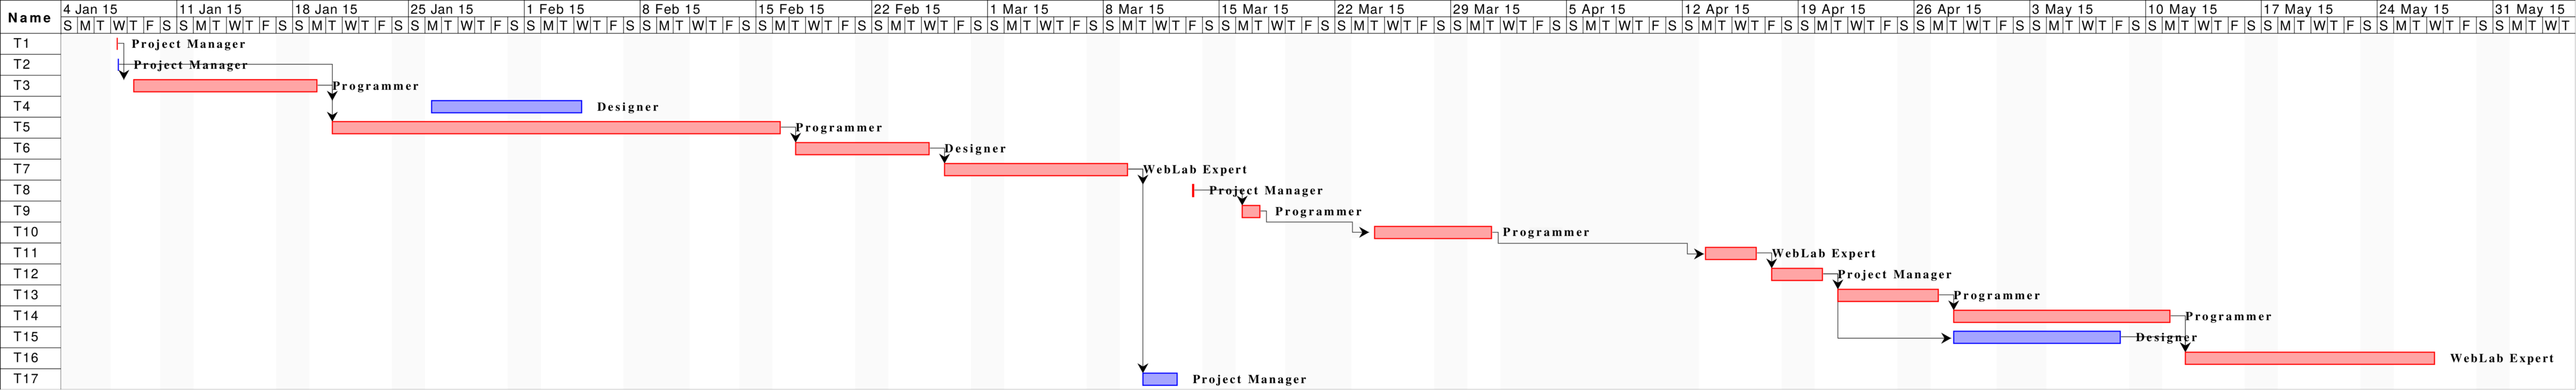
\includegraphics[trim=16.82in 0in 8in 0in, clip, angle=90]{fig/gantt}\clearpage
	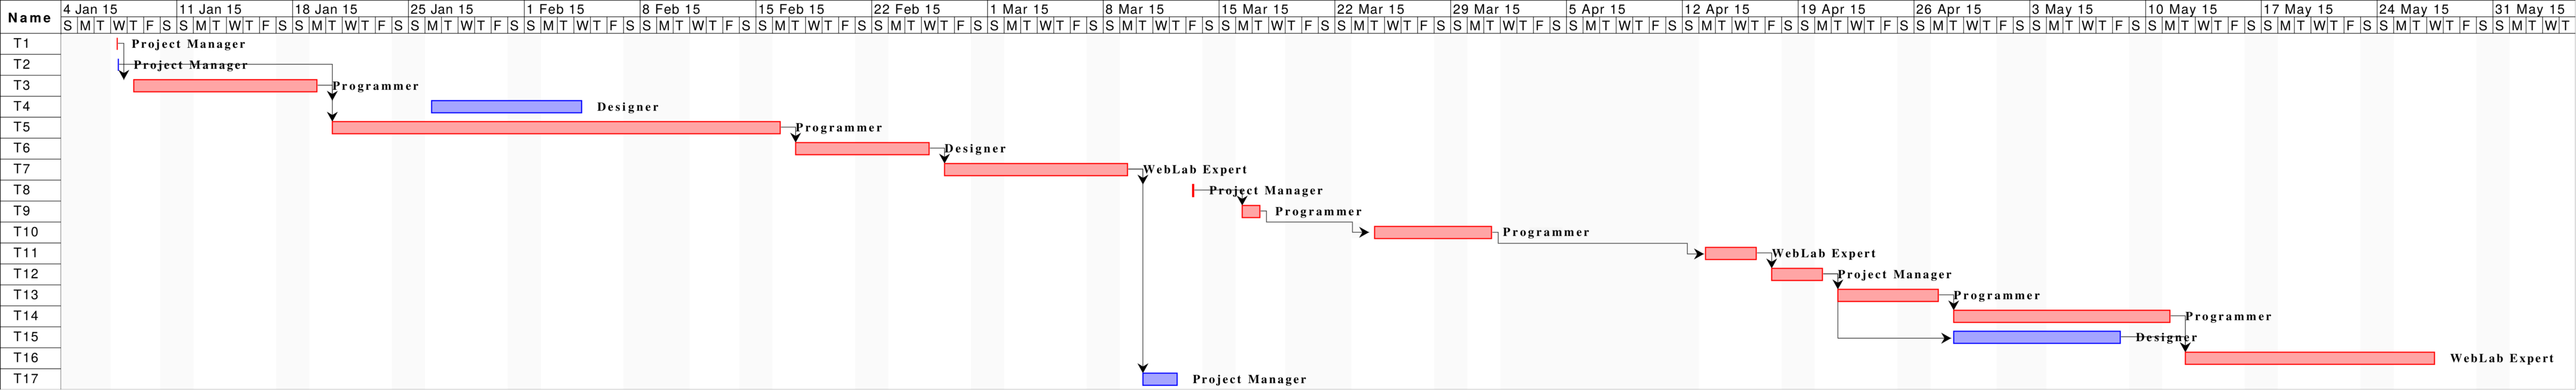
\includegraphics[trim=25.82in 0in 0in 0in, clip, angle=90]{fig/gantt}\clearpage
\end{center}

% Precedence diagram in four pages
\begin{figure}
	\centering
	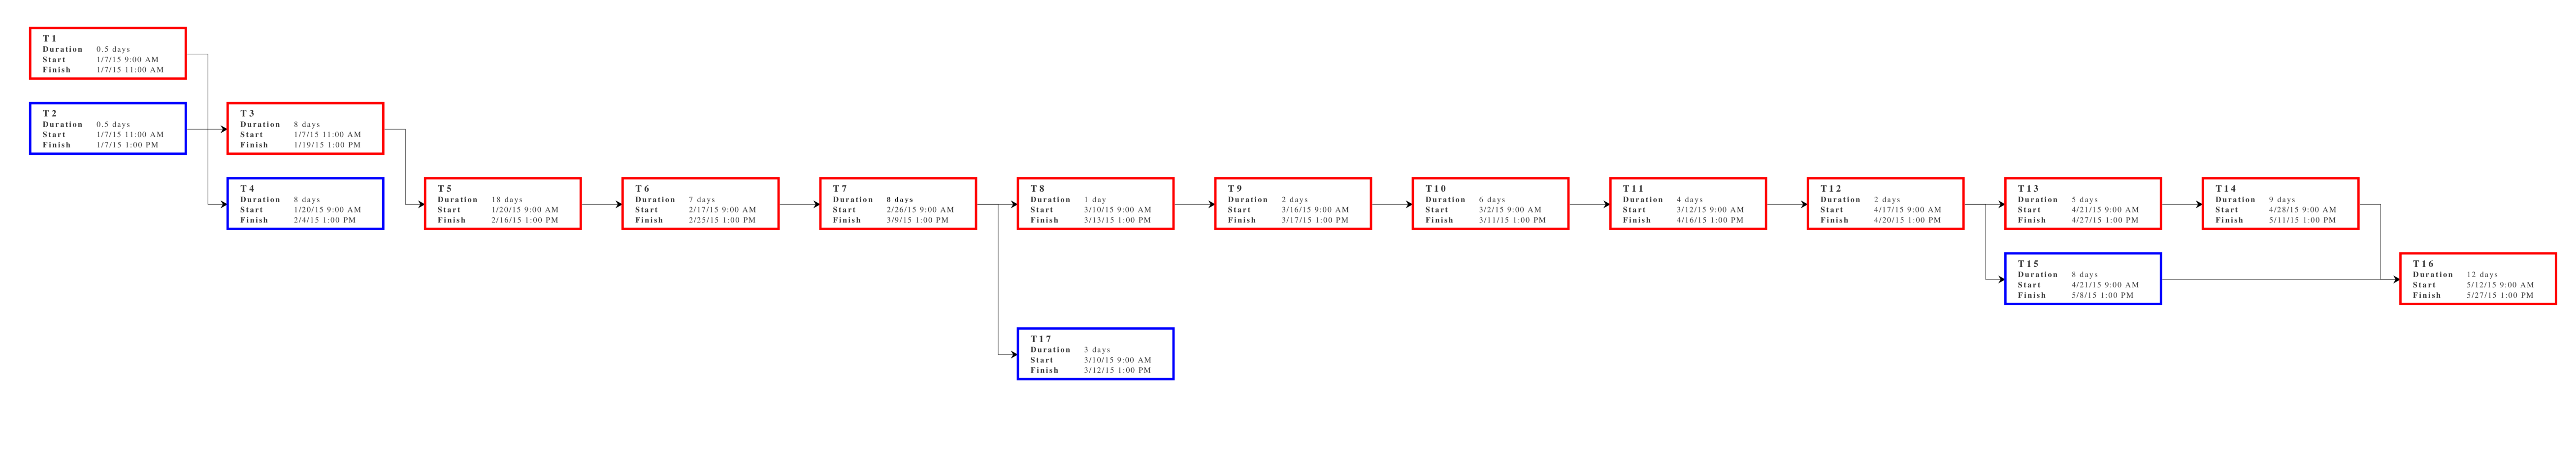
\includegraphics[trim=0in 0in 26in 0in, clip, angle=90]{fig/precedence}
	\caption[Precedence diagram of the project.]{Precedence diagram of the project. Continues in
	next pages.}\label{fig:precedence}
\end{figure}
\clearpage
\begin{center}
	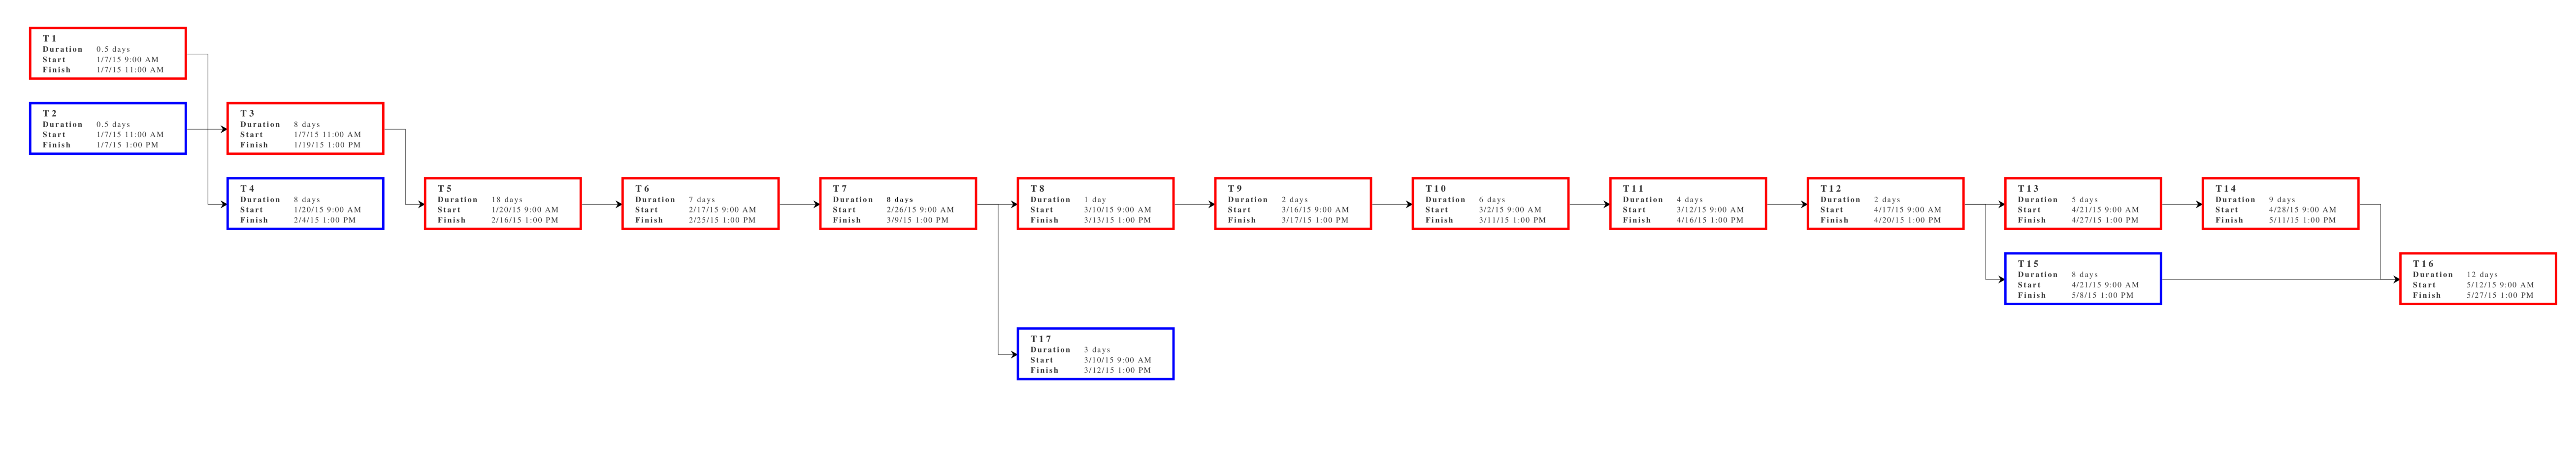
\includegraphics[trim=8.88in 0in 17in 0in, clip, angle=90]{fig/precedence}\clearpage
	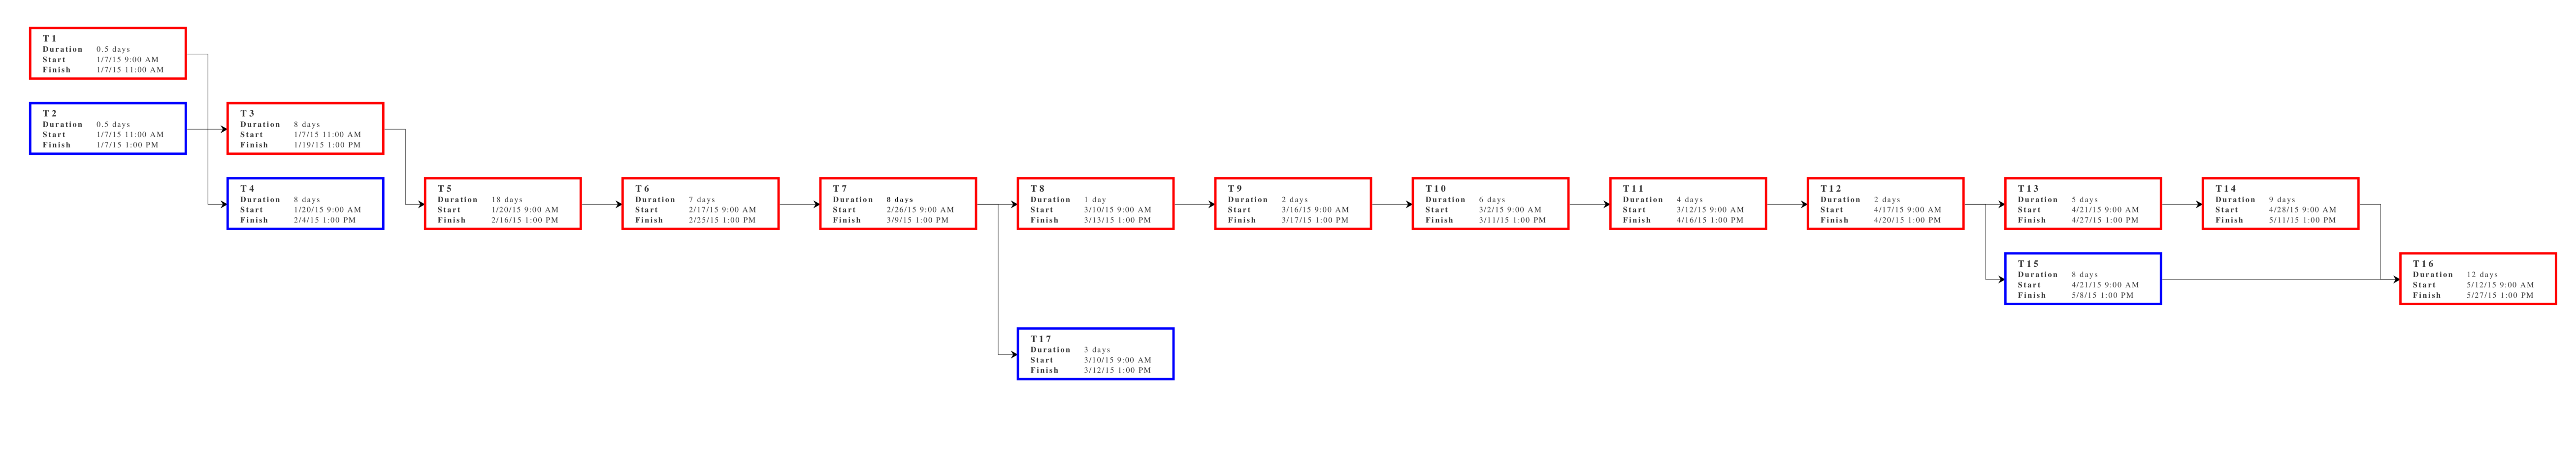
\includegraphics[trim=17.88in 0in 8in 0in, clip, angle=90]{fig/precedence}\clearpage
	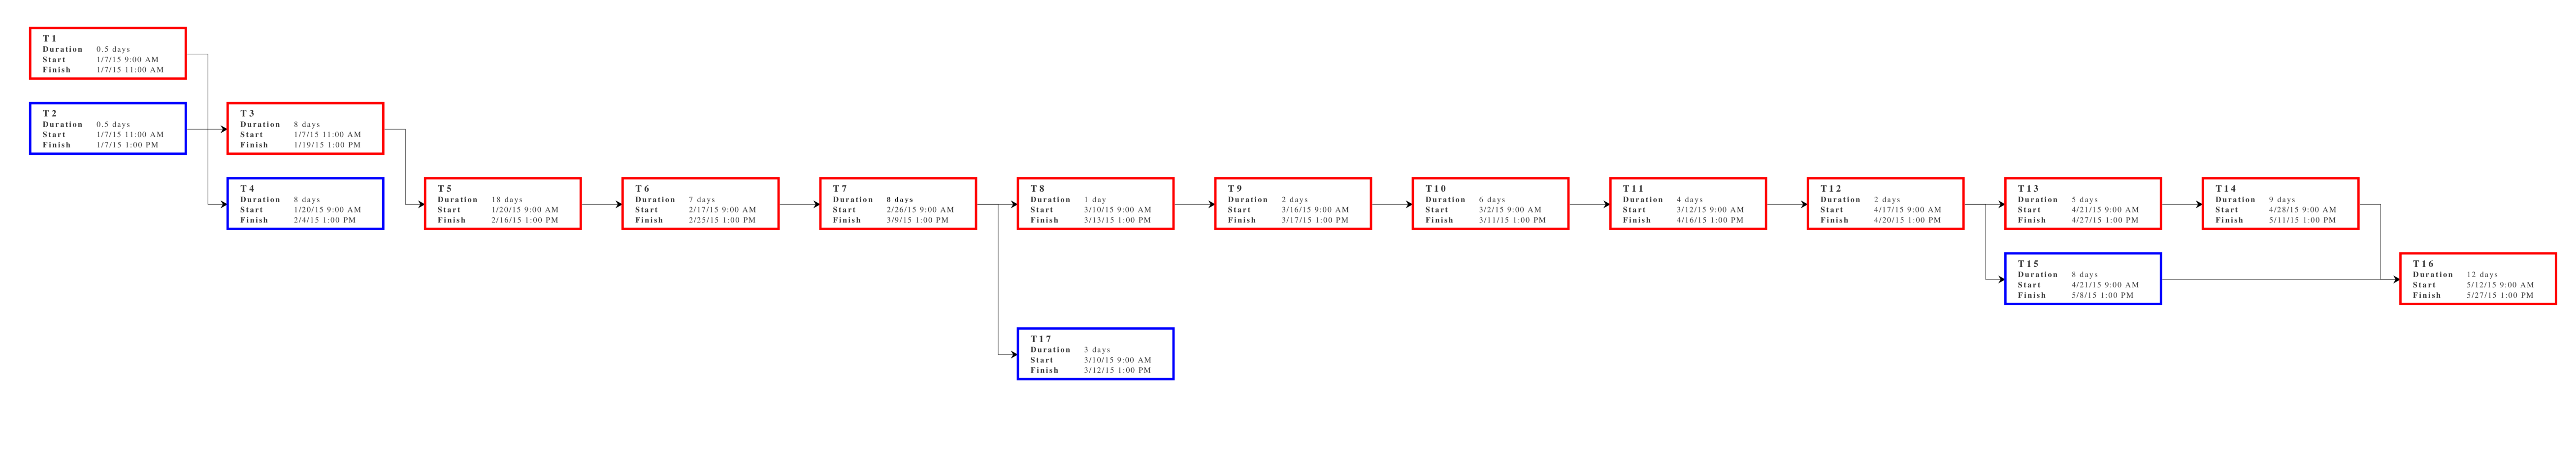
\includegraphics[trim=26.88in 0in 0in 0in, clip, angle=90]{fig/precedence}\clearpage
\end{center}

\chapter{Budget}

\chapter{Development}

\section{Trivia Game}

The first modality of the game is a trivia-type game, that will use Romie, the robot in
WebLab-Deusto and its labyrinth to create an experience for learning general knowledge. Moreover,
since the trivia questions will be configurable, so that the game can be adapted.

\subsection{Software and Hardware Requirements}

This software will have tight requirements in terms of user-friendliness, communication stability
and security, since it must be developed using as far as possible current hardware and be easy to
use by young students. Moreover, since it will be presented in crowded events, it must support high
load and availability.

Furthermore, due to the requirements of the project, it must be integrated with the WebLab-Deusto
platform and must be deployable in that environment. Thus, the requirements specification will be
as it follows:

\subsubsection{Software requirements:}

\begin{itemize}
	\item The software must be able to communicate with the robot.
	\item The software must be able to send control commands to the robot.
	\item The software must be able to receive command results from the robot.
	\item The software must be integrated in the WebLab-Deusto platform as a new experiment.
	\item The software must have an easy to use user interface based on human-computer interaction
	principles.
	\item The software must be stable enough to support tens of accesses per hour.
	\item The software must provide enough questions so that the user never finishes with them and
	can be randomly selected.
	\item The game must increase difficulty as the user gets more points.
	\item The game must finish in less than 15 minutes.
	\item A ranking must be provided after finishing the game for the user to know its ranking.
\end{itemize}

\subsubsection{Hardware requirements:}

\begin{itemize}
	\item The hardware must be placed in WebLab-Deusto.
	\item The robot must never get blocked, so in the case of an incident it must be automatically
	recovered.
	\item The cameras must be accessible from the Internet.
	\item The robot must be controlled via Bluetooth.
	\item The robot must never run out of power.
	\item The robot must be able to read all the \acrshort{rfid} tags with at least 99~\% accuracy.
	\item The robot must use the current labyrinth in WebLab-Deusto.
	\item No new hardware can be added to the current WebLab server (Plunder).
\end{itemize}

\subsection{Design Specification}

Taking into account the previous requirements, it has been decided to do a small hardware redesign
and a complete software design for the project. We will now see the hardware and software design
specifications.

\subsubsection{Hardware Specification}

Current robot is deployed with a simple \acrshort{rfid} (\acrlong{rfid}) reader (model ID-12) not
capable of reading further than 120~mm~\cite{rfid}, which has shown some issues when reading the
\acrshort{rfid} tags. For that reason, it has been decided to use a new module, the model ID-20LA
(figure~\ref{fig:rfid}). This will give the robot a much higher reliability when reading
\acrshort{rfid} tags, and the range of the new sensor is 180~mm~\cite{rfid}.

\begin{figure}[!htbp]
	\centering
	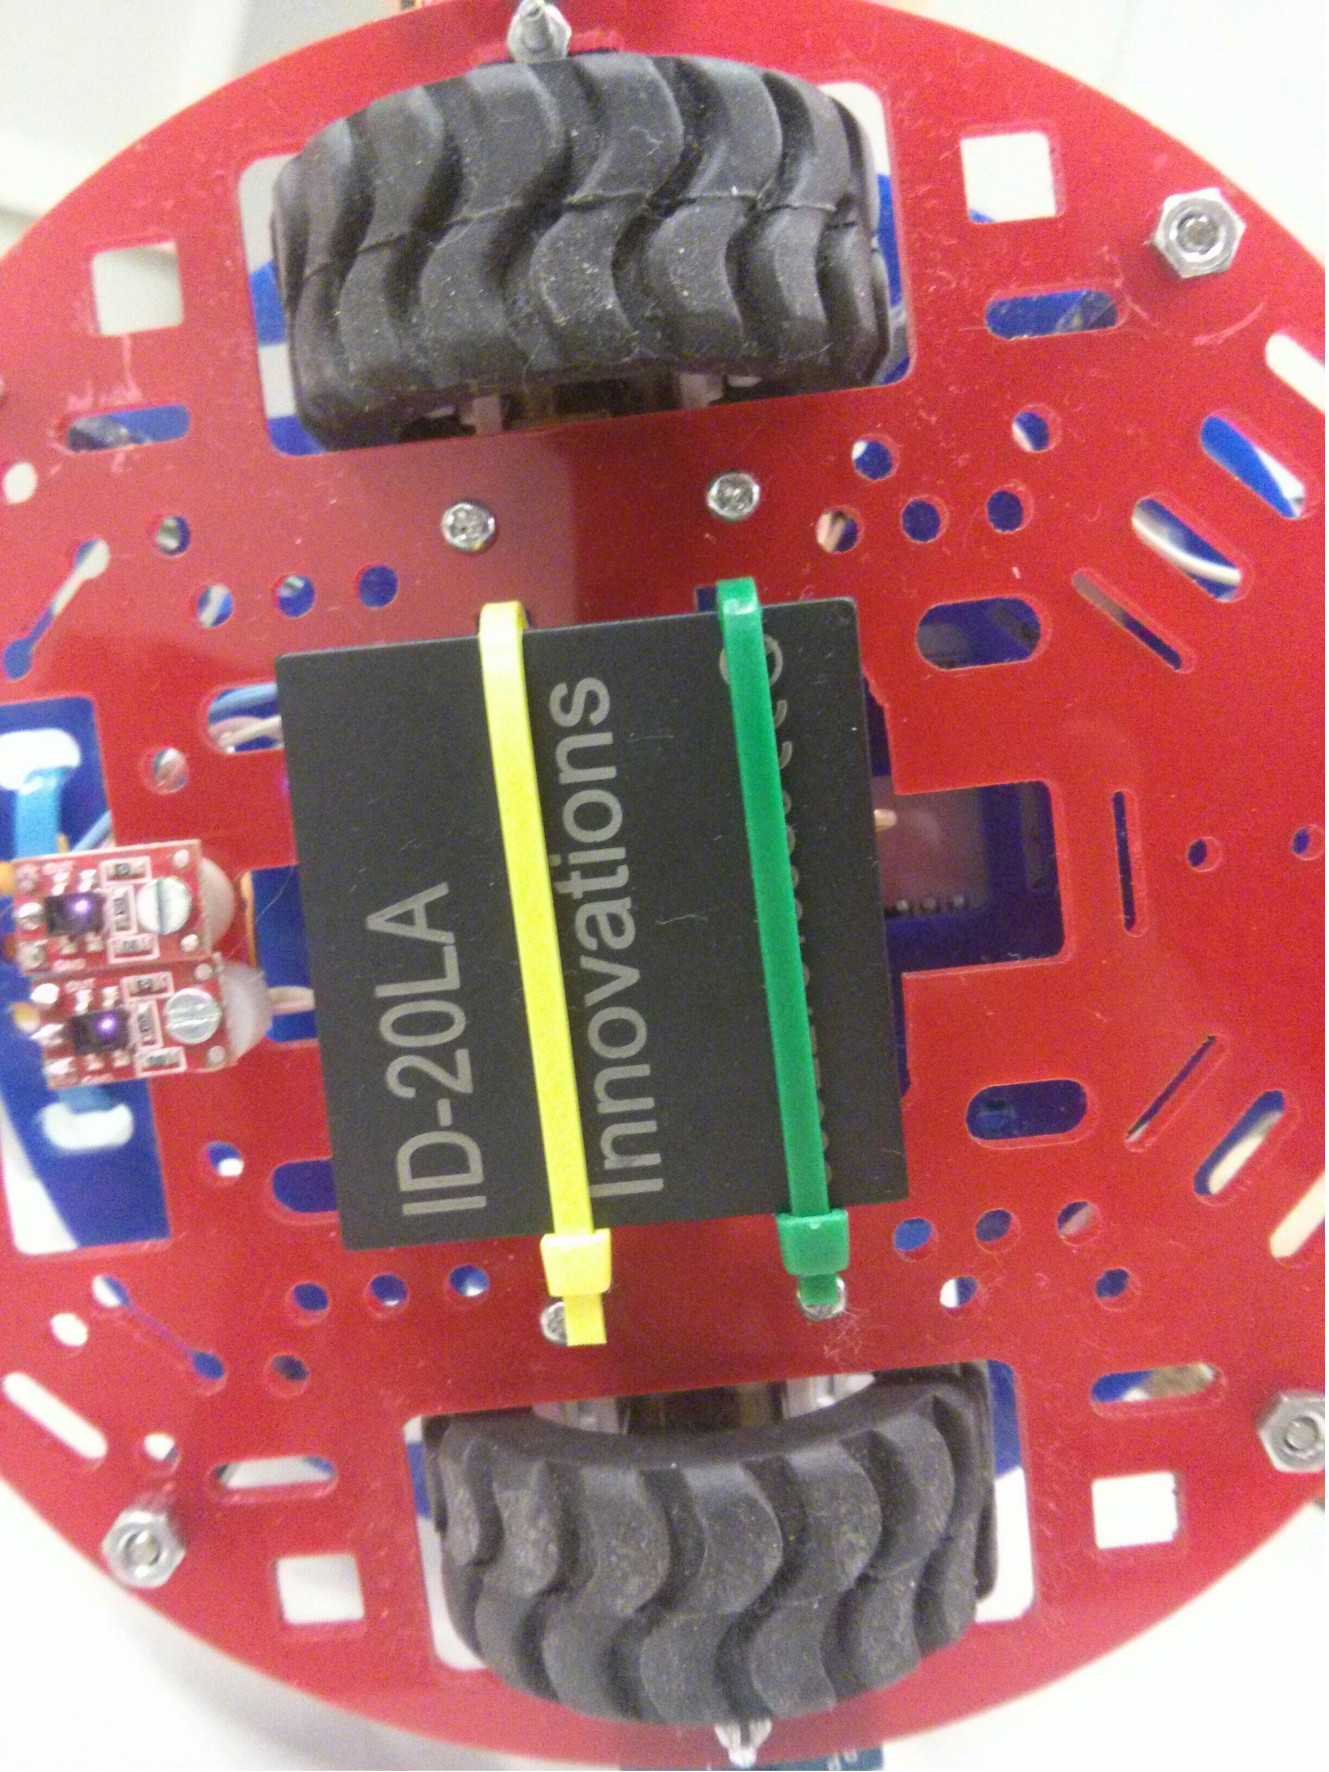
\includegraphics[width=0.3\textheight, angle=-90]{fig/rfid}
	\caption{ID-20LA \acrshort{rfid} reader.}
	\label{fig:rfid}
\end{figure}

On the other hand, there is currently an issue with the availability of the robot. It is powered
with a 2Ah \acrshort{lipo} battery, and is recharged when needed. This has a big issue, since as we
have seen, in high load conditions would not meet the required availability, and furthermore, in
weekends or holidays, we will not be able to change and recharge the battery, so it has been decided
to deploy a cable installation from the roof of the ceiling of the laboratory, and the design of the
robot has been adapted so that the cables do not get stuck in the labyrinth.

The rest of the robot will be used as it is, since it provides with the needed capabilities for the
needs of the project: It has a wall sensor capable of avoiding crashes with walls, infrared sensors
to detect the lines in the ground, motors and wheels capable of moving the robot, Bluetooth
connection to communicate with it and Arduino microcontroller, to install the needed firmware
(figure~\ref{fig:bluetooth}).

\begin{figure}[!htbp]
	\centering
	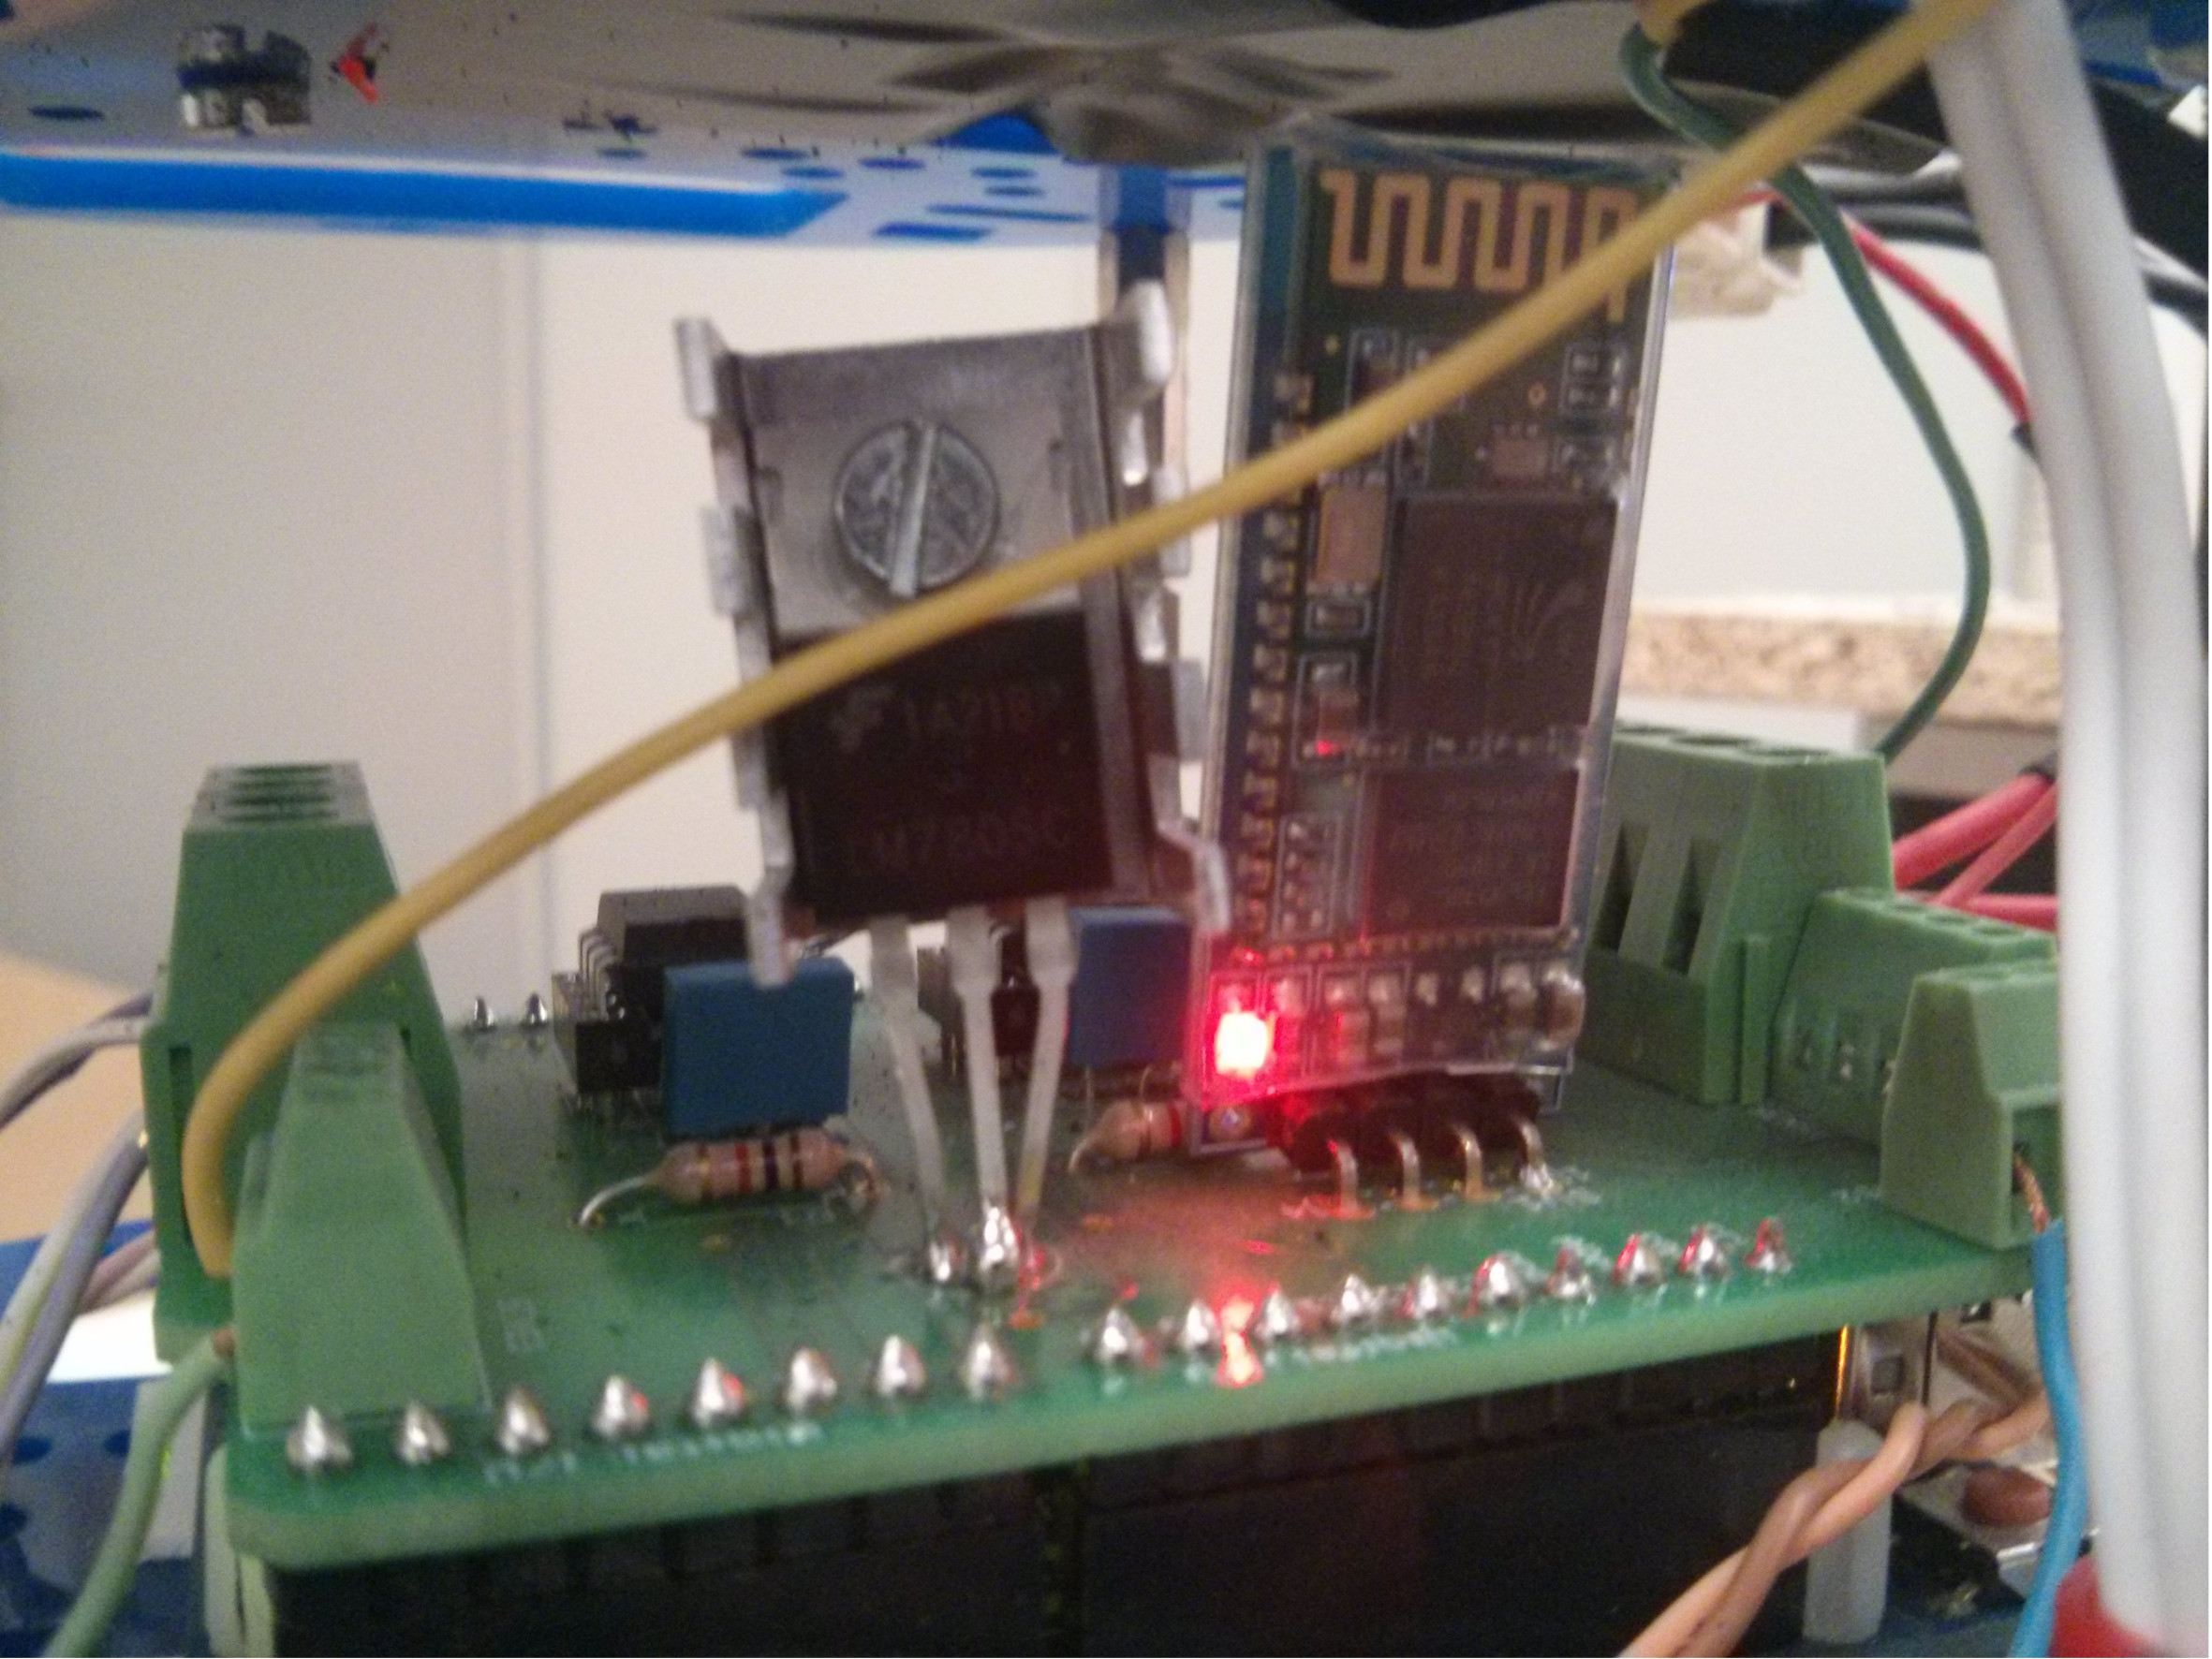
\includegraphics[width=0.65\textwidth]{fig/bluetooth}
	\caption{Bluetooth module on top of the Arduino shield.}
	\label{fig:bluetooth}
\end{figure}

The robot is currently configured with a camera D-link DCS-932L that provides infrared vision if the
light is shut down and normal vision if not, and it can be accessed from Wi-Fi and
Ethernet~\cite{camera}. In this case we will use it via Wi-Fi, since the robot will be moving around
a big space.

\subsubsection{Software Specification}

The software in for this implementation will be divided modularly, thinking on scalability and
code reuse. The application must be built on top of WebLab-Deusto, so we will use as much as
possible the provided \acrshort{api}s. Moreover, and due to deployment needs, the software will be
divided between the robot, an intermediate server and WebLab software.

The robot will use a slightly modified version of the current firmware, since we need it not to get
blocked by any wall in case of crash and we need a more reliable implementation. That is why it has
been programmed to turn back if a hardware error occurs and collides with a wall. Nevertheless, the
external Bluetooth \acrshort{api} will be the same as the one that was already implemented at the
beginning of the project:

It will provide a ``F'' command to go forward, that will return the \acrshort{rfid} tag if it finds
one, a ``L'' command to turn left, its counterpart ``R'' command to turn right and it will also
provide the command ``S'' that will check if there is a wall in front of the robot. Nevertheless,
and even if the experiment server can check for a wall, the robot itself has been programmed to
return a ``NAK'' command if it is commanded to go forward against a wall.

The robot itself works following the lines in the labyrinth until it finds an intersection. It is
also capable of turning in those intersections, so if it is commanded to turn right, it will perform
a 90 degree turn right and face the path in its right. When the robot stops on top of a
\acrshort{rfid} tag, it will return the tags address.

The intermediate server will provide a small \acrlong{rest} (\acrshort{rest}) \acrshort{api} in a
small Python server. Its only duty will be to provide a simple interface for the robot using
\acrshort{http} instead of Bluetooth, needed due to deployment constraints. We can see an example of
the \acrshort{api} usage with Python in algorithm~\ref{alg:romie_rasp}.

\begin{center}
\begin{minipage}{.9\textwidth}
\singlespace
\begin{pyglist}[language=python, caption={Romie \acrshort{rest} \acrshort{api} example.},
	label={alg:romie_rasp}, listingname={Algorithm}, numbers=left]
import urllib2

# Let's go forward and get RFID tag if exists
tag = urllib2.urlopen('http://192.168.0.190:8000/f', timeout = 60).read()

# Let's turn left
result = urllib2.urlopen('http://192.168.0.190:8000/l', timeout = 60).read()

# Let's turn right
result = urllib2.urlopen('http://192.168.0.190:8000/r', timeout = 60).read()

# Let's check if we have a wall in front of us
result = urllib2.urlopen('http://192.168.0.190:8000/s', timeout = 60).read()
\end{pyglist}
\end{minipage}
\end{center}

Then, the experiment server required by the WebLab-Deusto architecture, will provide a WebLab
command \acrshort{api}, that will be callable by the client of the experiment. This server will be
developed in Python because the WebLab server libraries are better intended for this language. The
data for the ranking will be stored in a SQLite 3 database. This database provides all the needed
\acrshort{acid} constraints (\acrlong{acid}) with a small \acrshort{sql} (\acrlong{sql}) a
\acrlong{rdbms} (\acrshort{rdbms})~\cite{sqlite}.

The experiment server \acrshort{api} will have all the needed commands to use the experiment. For
the ones that need data being sent to the server, \acrshort{json} has been used (\acrlong{json}). It
is preferred over \acrshort{xml} (\acrlong{xml}) due to the higher compatibility of \acrshort{json}
and the more data-orientation of this \acrlong{rfc} or \acrshort{rfc}. This provides lower
overhead~\cite{xml_vs_json}.

\begin{itemize}
	\item ``\textbf{F}'', ``\textbf{L}'' and ``\textbf{R}'' commands, to move forward and turn left
	and right. The ``S'' command is not provided since the experiment does not require it and the
	robot will not drive towards a wall. The ``\textbf{F}'' will return a random question based on
	the current user's points.

	\item ``\textbf{CHECK\_REGISTER}'' command, to check if the user has been registered in the
	experiment before and decide if the experiment should show the registration form.

	\item ``\textbf{REGISTER}'' command, to send the registration data to the server and insert it
	into the SQLite database.

	\item ``\textbf{ANSWER}'' command, to send the answer given by the user to a question. It will
	return the new date for finishing the experiment and the new points for the user. These will not
	change if the answer was not correct.

	\item ``\textbf{FINISH}'' command, to finish the experiment and receive the final ranking.
\end{itemize}

Finally, the client will be developed using \acrshort{html} 5 (\acrlong{html} version 5), JavaScript
(using JQuery library) and Bootstrap for a rapid development. It will use the WebLab JavaScript
library to communicate with the experiment server. This library is an asynchronous \acrshort{ajax}
(\acrlong{ajax}) library that provides a simple interface to interact with experiments. We can see
an example in algorithm~\ref{alg:weblab_lib}.

\begin{center}
\begin{minipage}{.9\textwidth}
\singlespace
\begin{pyglist}[language=javascript, caption={WebLab JavaScript library example.},
	label={alg:weblab_lib}, listingname={Algorithm}, numbers=left]
// Callback registration that will be
// called after reserving the experiment
Weblab.setOnStartInteractionCallback(start);

// Sending command to the experiment server
Weblab.sendCommand("L", function(response) {
    console.log("Good response: " + response);
}, function(response) {
    console.log("Bad response: " + response);
});
\end{pyglist}
\end{minipage}
\end{center}

TODO: Software design graphic (experiment flow chart)

\subsection{Deployment Considerations}

The deployment must be done in WebLab-Deusto, a remote laboratory environment with three custom
networks and limited physical space. In figure~\ref{fig:weblab-network} we can see the network of
WebLab-Deusto. As we can see, Plunder is the core server. It provides access to WebLab-Deusto web
environment and it provides most of the experiment servers. On the other hand, Blood is the one
working as a proxy for all the cameras in WebLab-Deusto, some of them connected by Wi-Fi and others
by Ethernet.

\begin{figure}[!htbp]
	\centering
	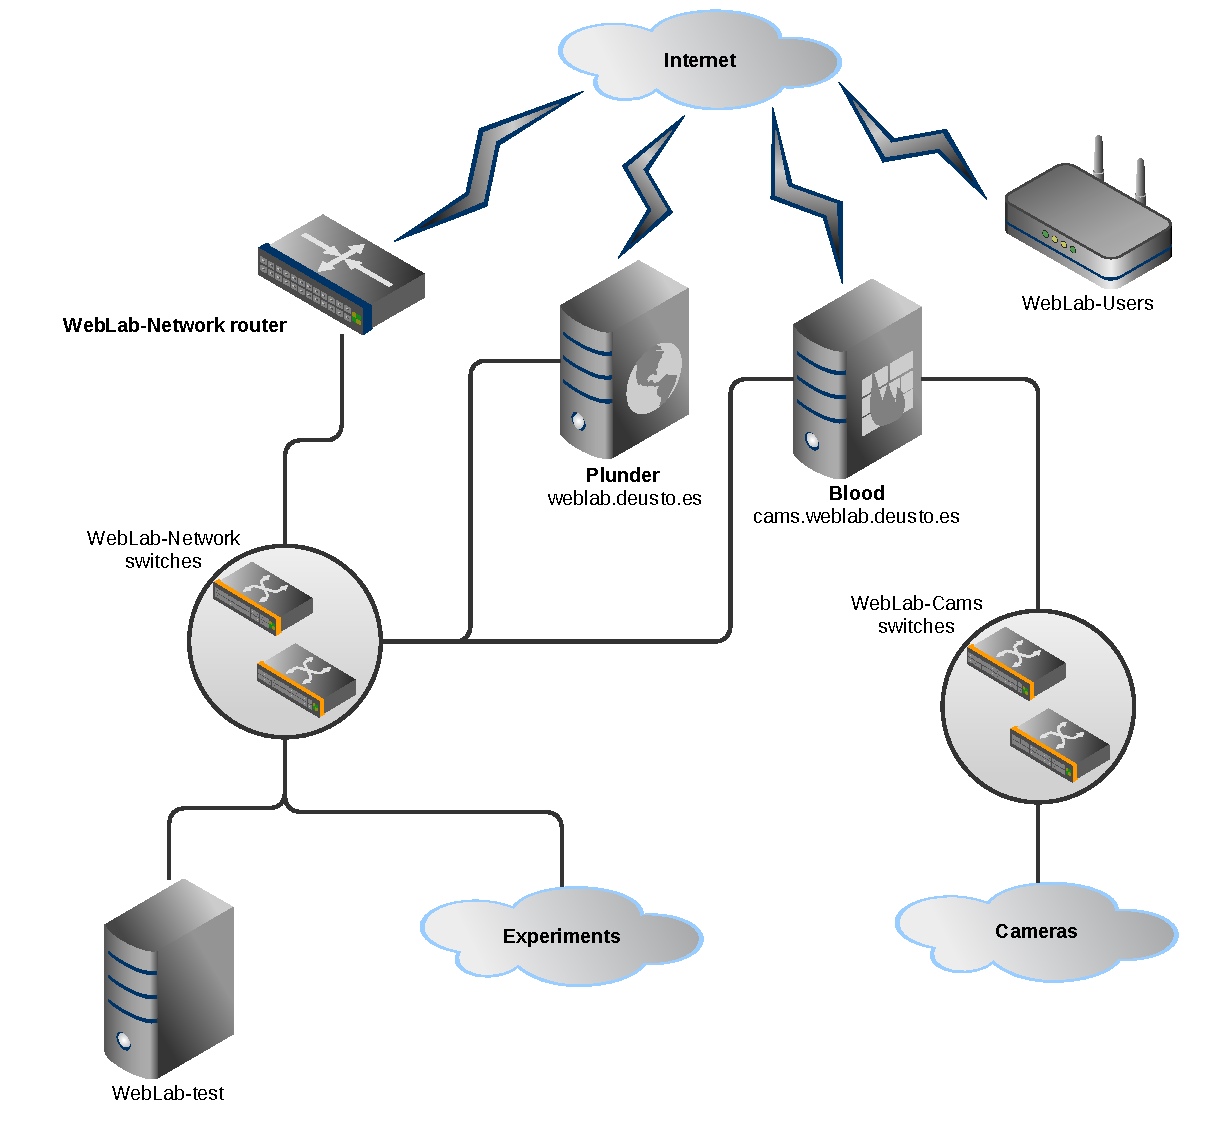
\includegraphics[width=0.9\textwidth]{fig/weblab-network}
	\caption{WebLab-Deusto network simplification.}\label{fig:weblab-network}
\end{figure}

In this case, since we need Bluetooth to connect our experiment server to the robot, and Plunder,
Blood and WebLab-test should not need new hardware, we will use a Raspberry Pi Model B
(figure~\ref{fig:rasp}) with a \acrshort{usb} (\acrlong{usb}) Bluetooth dongle to connect to the
robot and to provide a simple \acrshort{http} server with the \acrshort{rest} \acrshort{api}. This
small computer provides us with the needed hardware for such small web server, since it provides
512~MB of \acrshort{ram}, a 700~Mhz \acrshort{arm} \acrshort{cpu}, 2 \acrshort{usb} ports and an
Ethernet port. All this in a small form factor, not bigger than a usual credit card, and consuming
only 3.5~W.

\begin{figure}[!htbp]
	\centering
	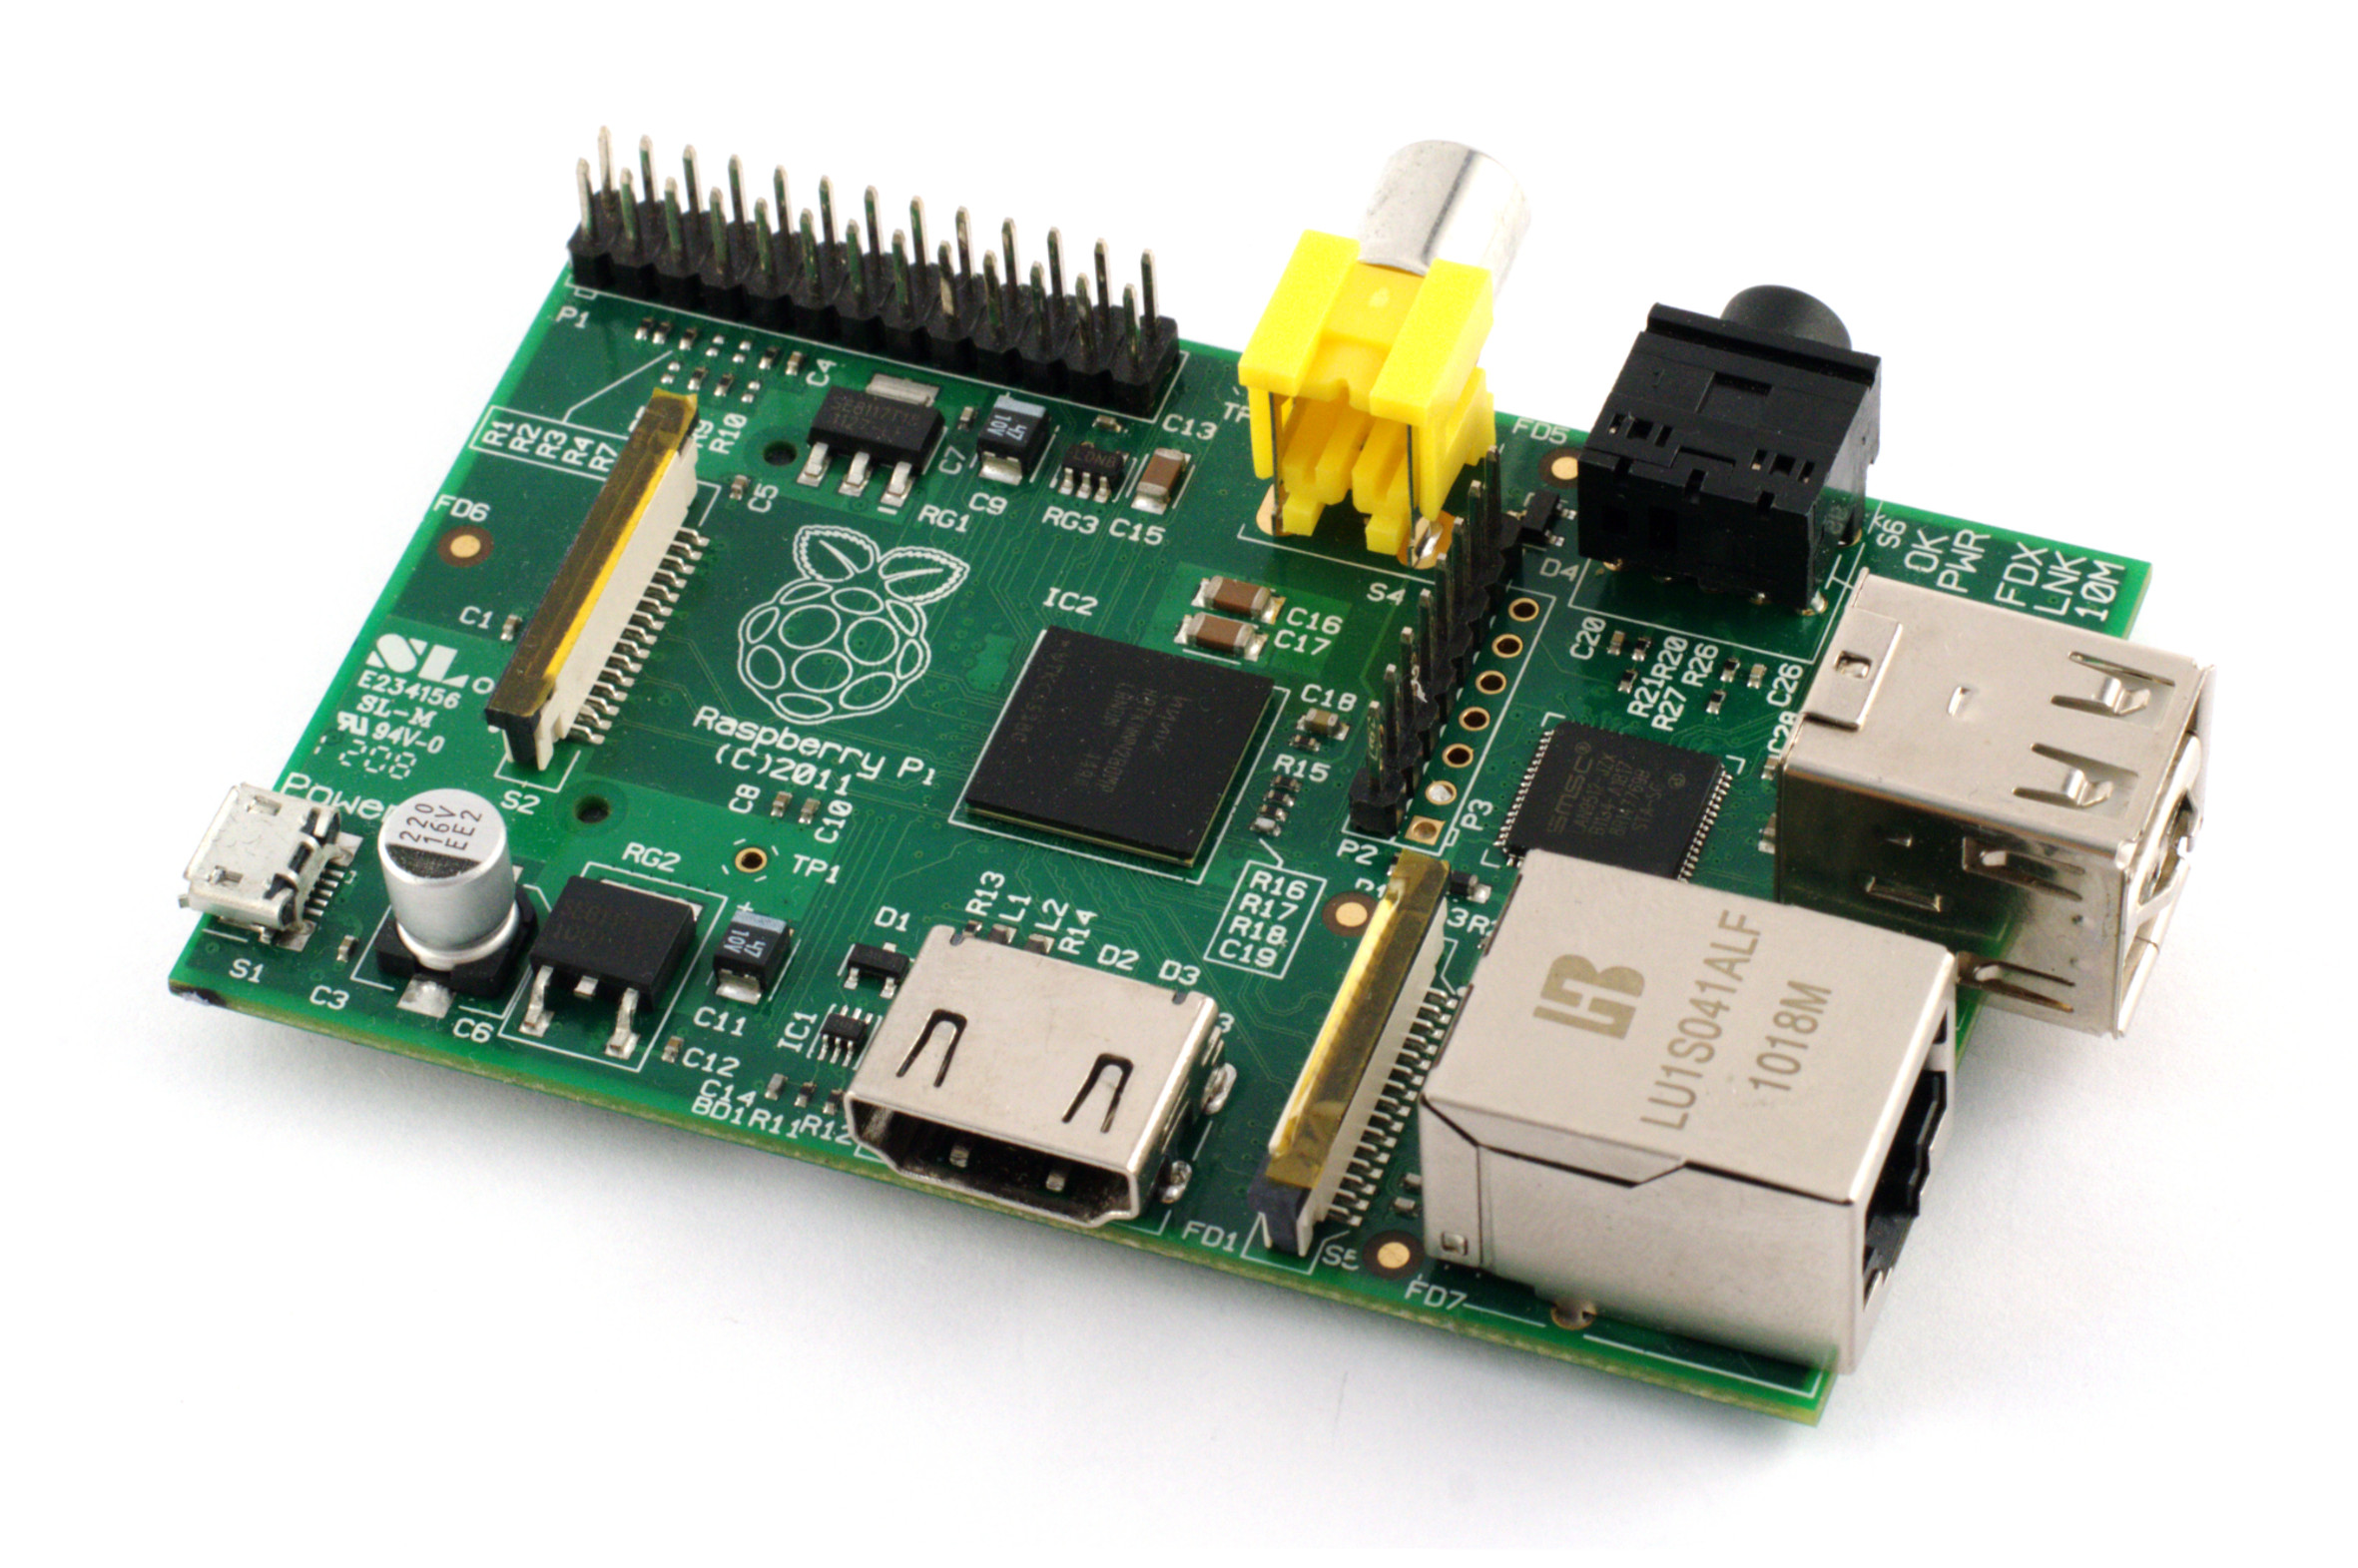
\includegraphics[width=0.7\textwidth]{fig/rasp}
	\caption{Raspberry Pi model B computer.}
	\label{fig:rasp}
\end{figure}

This small computer will be connected via Ethernet to the WebLab network, while two cameras (the top
camera and the on-board camera) will be connected via Wi-Fi to WebLab camera network, using Blood as
the \acrshort{http} proxy server.

Finally, since the server software will change many times during the development, and Plunder must
be restarted for each change if the experiment server is located there, the experiment server for
this experiment will be located in WebLab-test. This way, there will be no need to restart Plunder
each time a new change is made to the experiment, giving higher availability to WebLab-Deusto.

\subsection{Testing Plan}

The testing for this software is divided in 3 main environments. First of all, the usual manual
testing is made by the developers and by the administrators of WebLab-Deusto. This showed many bugs
that we were able to fix almost as soon as they appeared, but in any case, this is not enough
for a production environment.

After the manual testing, WebLab-Deusto has a \acrlong{ci} system connected to Travis \acrshort{ci}
in GitHub. It provides many unit tests that provide stability to the code, since we receive emails
when a commit does not pass the tests. Nevertheless, for the \acrlong{gui} or \acrshort{gui}, it is
difficult to provide unit tests.

Finally, and also as a demonstration of the potential of the project, we tested the project in an
event at the University of Deusto called ForoTech~\cite{forotech}. In this event we were be able to
test the project in a high load environment, where the robot received more than a hundred uses in a
short period of time, demonstrating the reliability and also giving us the possibility to fix some
issues.

\subsection{User Manual}

For using Romie, you must have an account in WebLab-Deusto and the appropriate permissions to use
the experiment. Once you fulfill those requirements, go to
\url{https://weblab.deusto.es/weblab/client/}. In that page (figure~\ref{fig:man:weblab}), you will
be able to insert your credentials in the login form and log in.

\begin{figure}[ht]
	\centering
	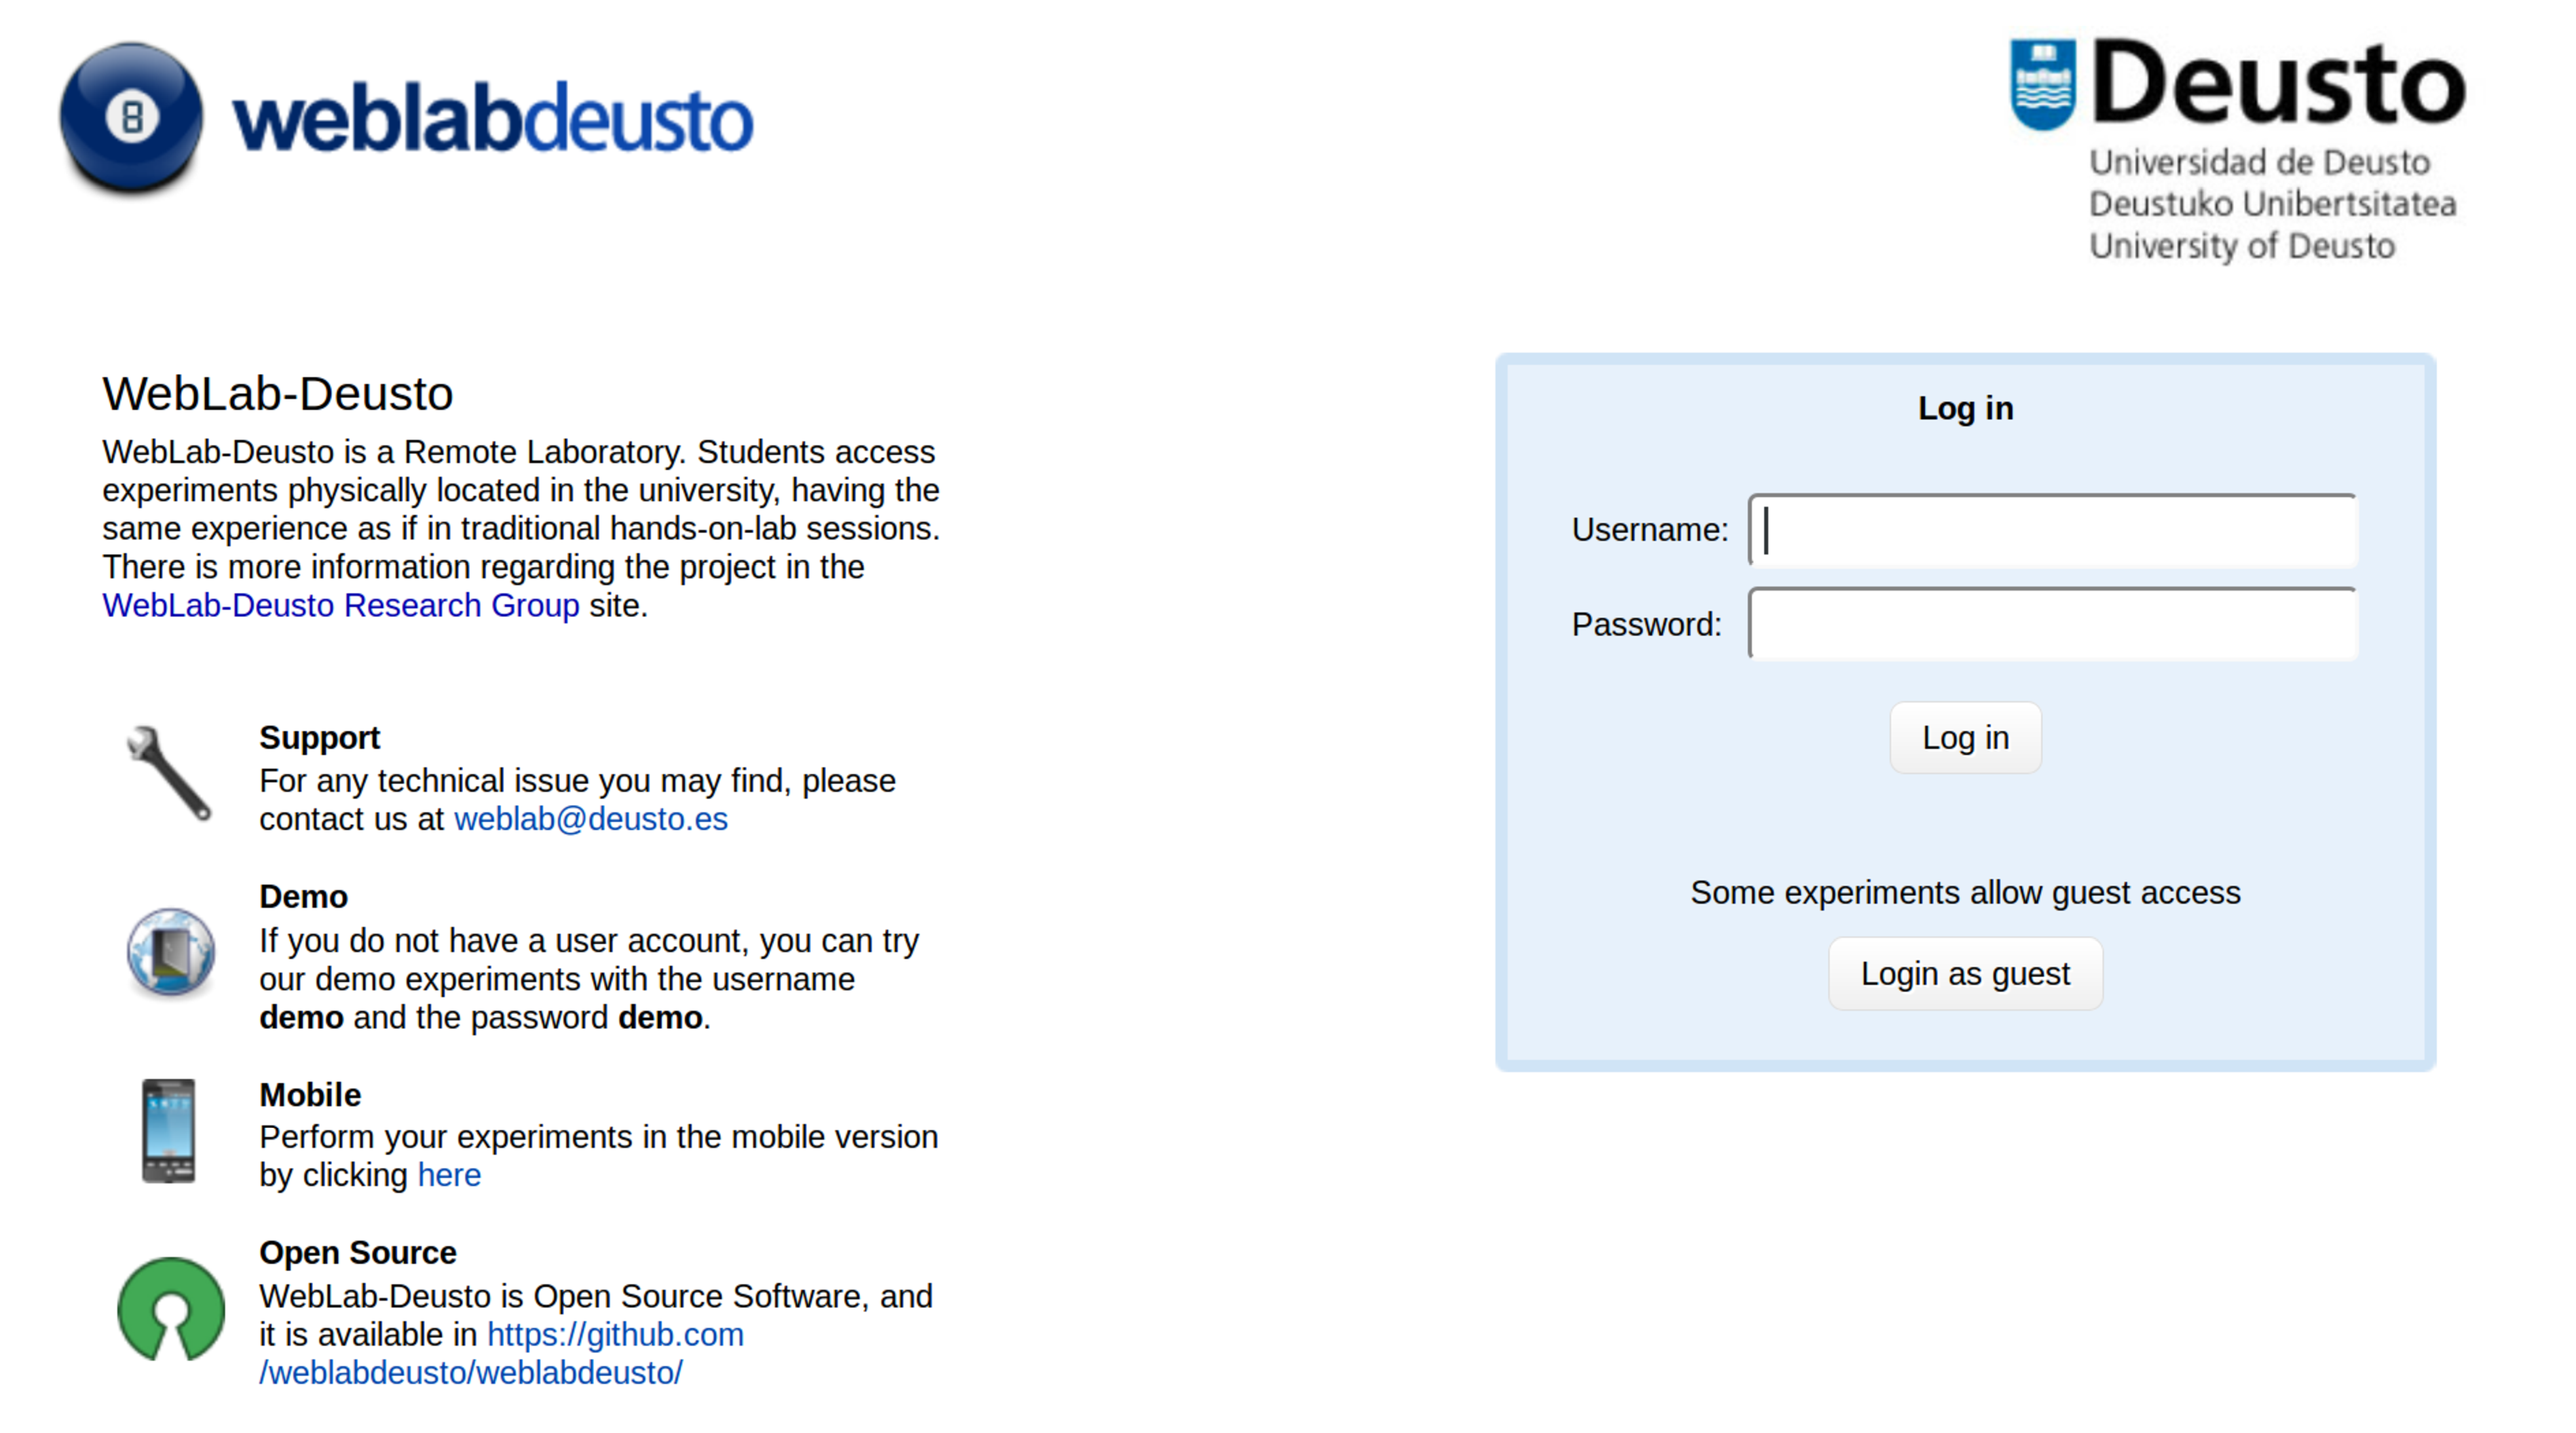
\includegraphics[width=0.75\textwidth]{fig/manuals/weblab}
	\caption{WebLab Deusto's landing page.}
	\label{fig:man:weblab}
\end{figure}

Once logged in, you will see ``romie'' experiment under the ``Robot experiments'' category
(figure~\ref{fig:man:romie_weblab}). You could see more experiments if you have the permission to
use them. If you cannot find the experiment you should contact with the administrators. Click on
``romie'' or in its image and you will enter the reservation page
(figure~\ref{fig:man:romie_reserve}). There, you can reserve the experiment clicking the ``Reserve''
button.

\begin{figure}[!htbp]
	\centering
	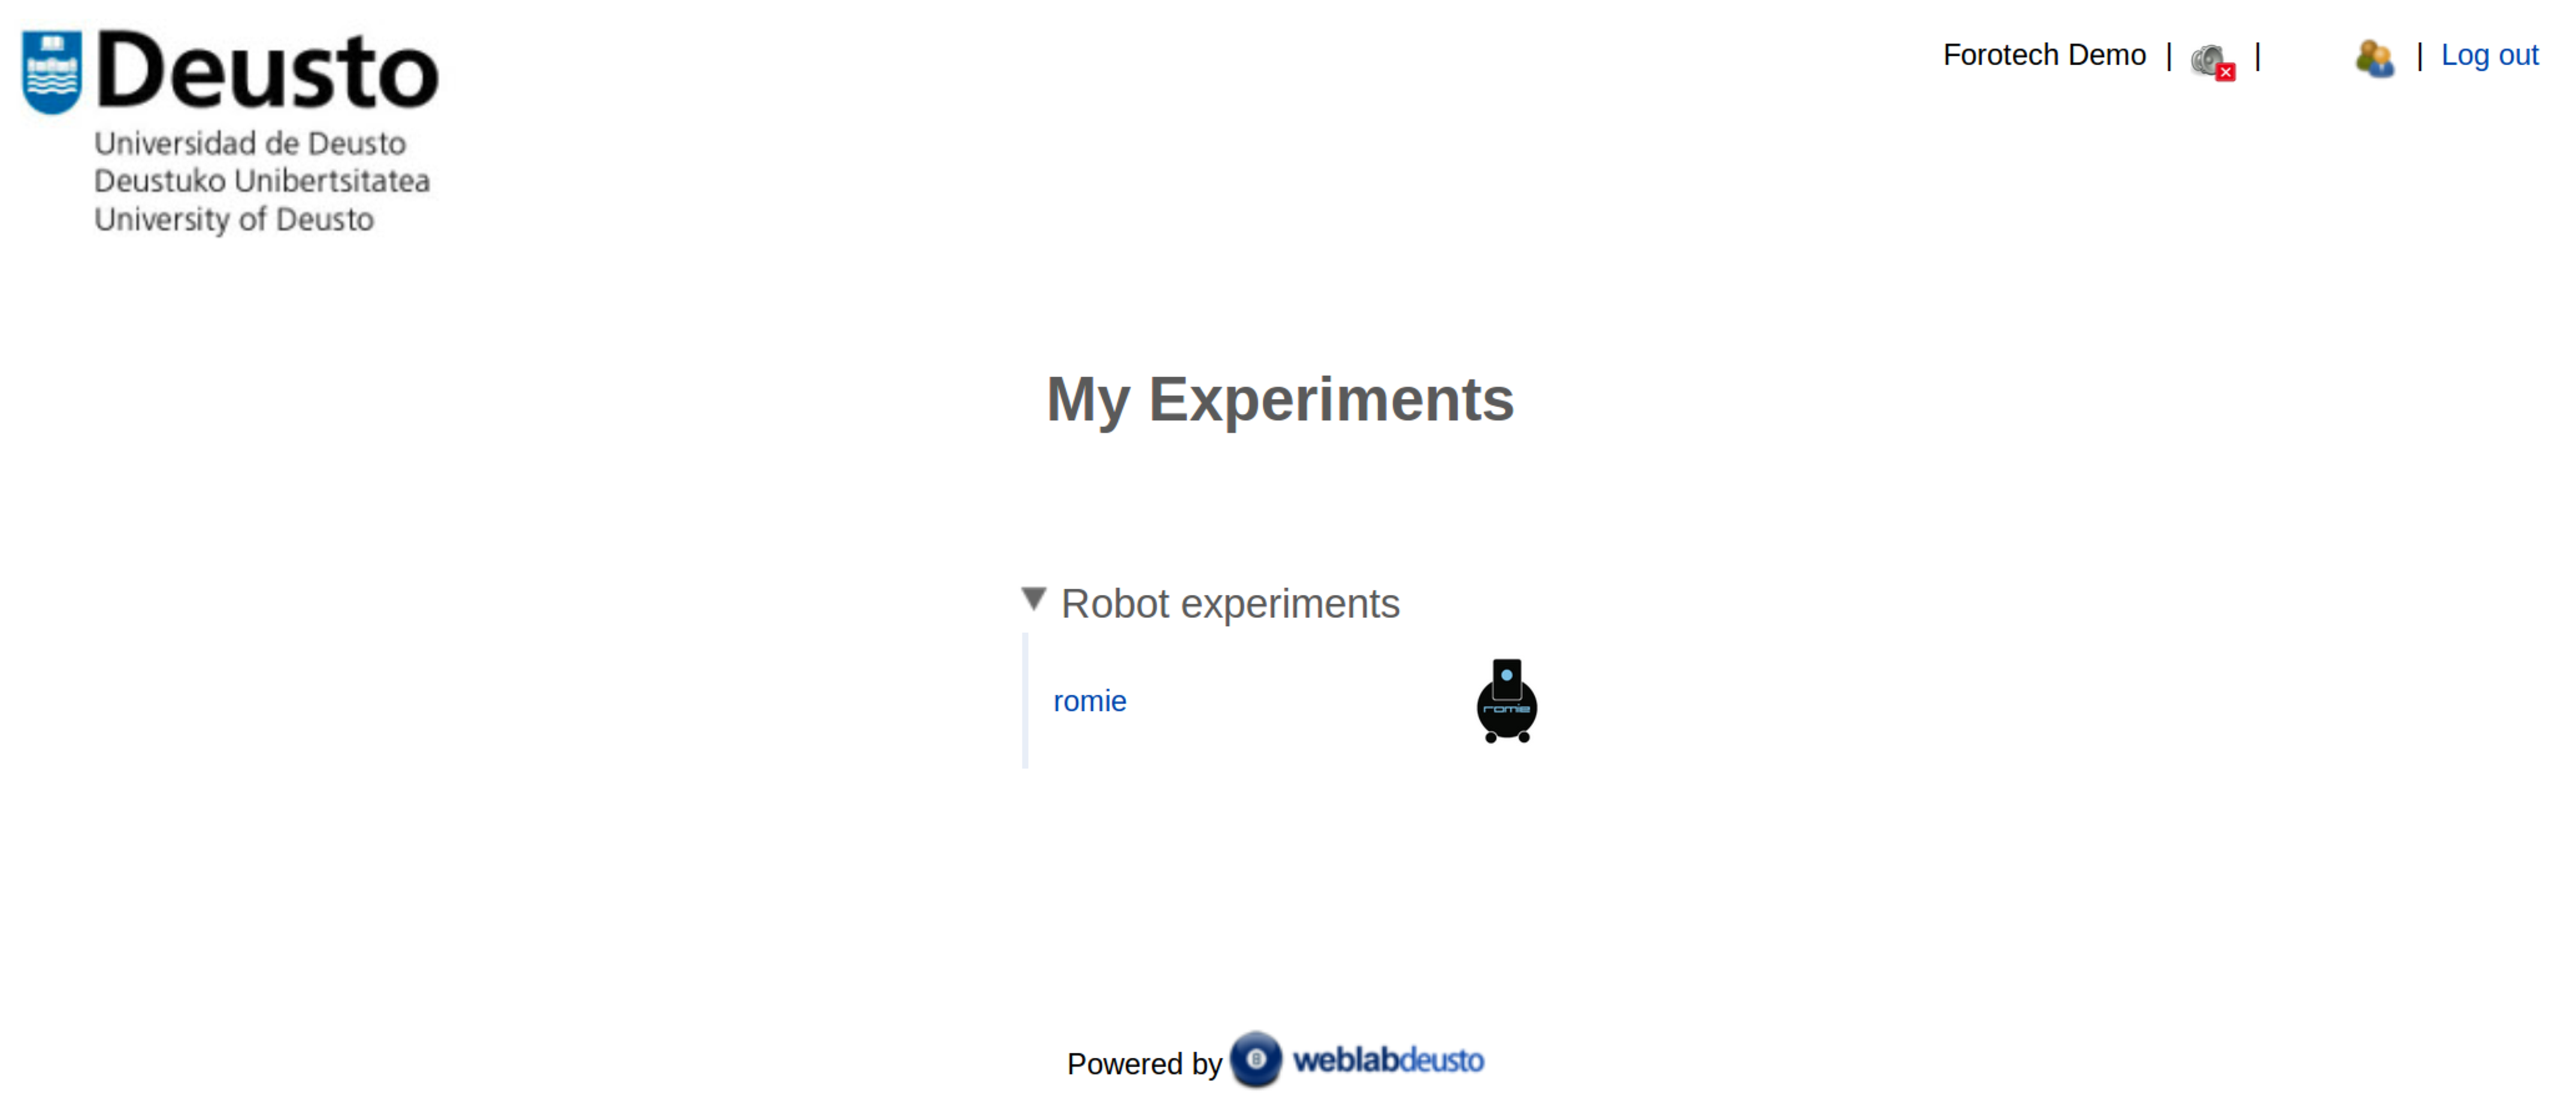
\includegraphics[width=0.85\textwidth]{fig/manuals/trivia/romie-weblab}
	\caption{Romie under ``Robot experiments'' in WebLab Deusto.}
	\label{fig:man:romie_weblab}
\end{figure}

\begin{figure}[!htbp]
	\centering
	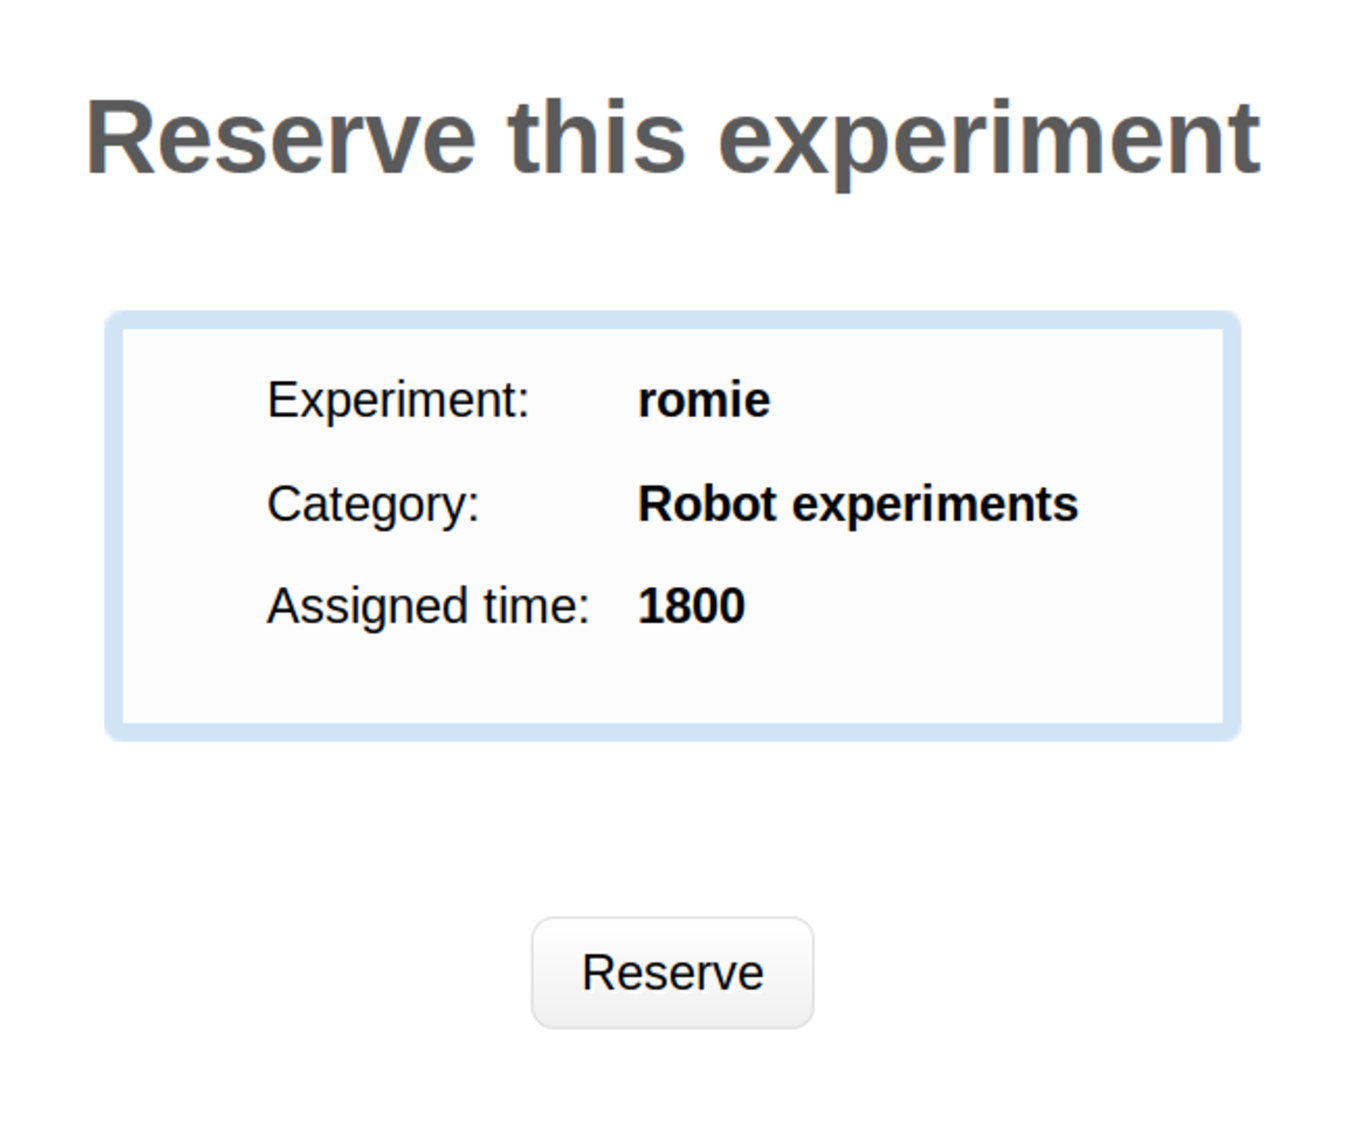
\includegraphics[width=0.5\textwidth]{fig/manuals/trivia/romie-reserve}
	\caption{Romie reservation screen.}
	\label{fig:man:romie_reserve}
\end{figure}

Once reserved, on the first use, you will see the registration form
(figure~\ref{fig:man:romie_register}). You will have to fill it in order to play the game. There is
also a version without the registration screen if you only want to test the robot, ask the
administrators for permission to use it. After filling the registration form  with your own data,
you can click the register button. \emph{Note: the experiment is prepared to work with students of
less than 18 years old, so any age above that or below 5 years old is considered an input error,
that will be notified in the interface}.

\begin{figure}[!htbp]
	\centering
	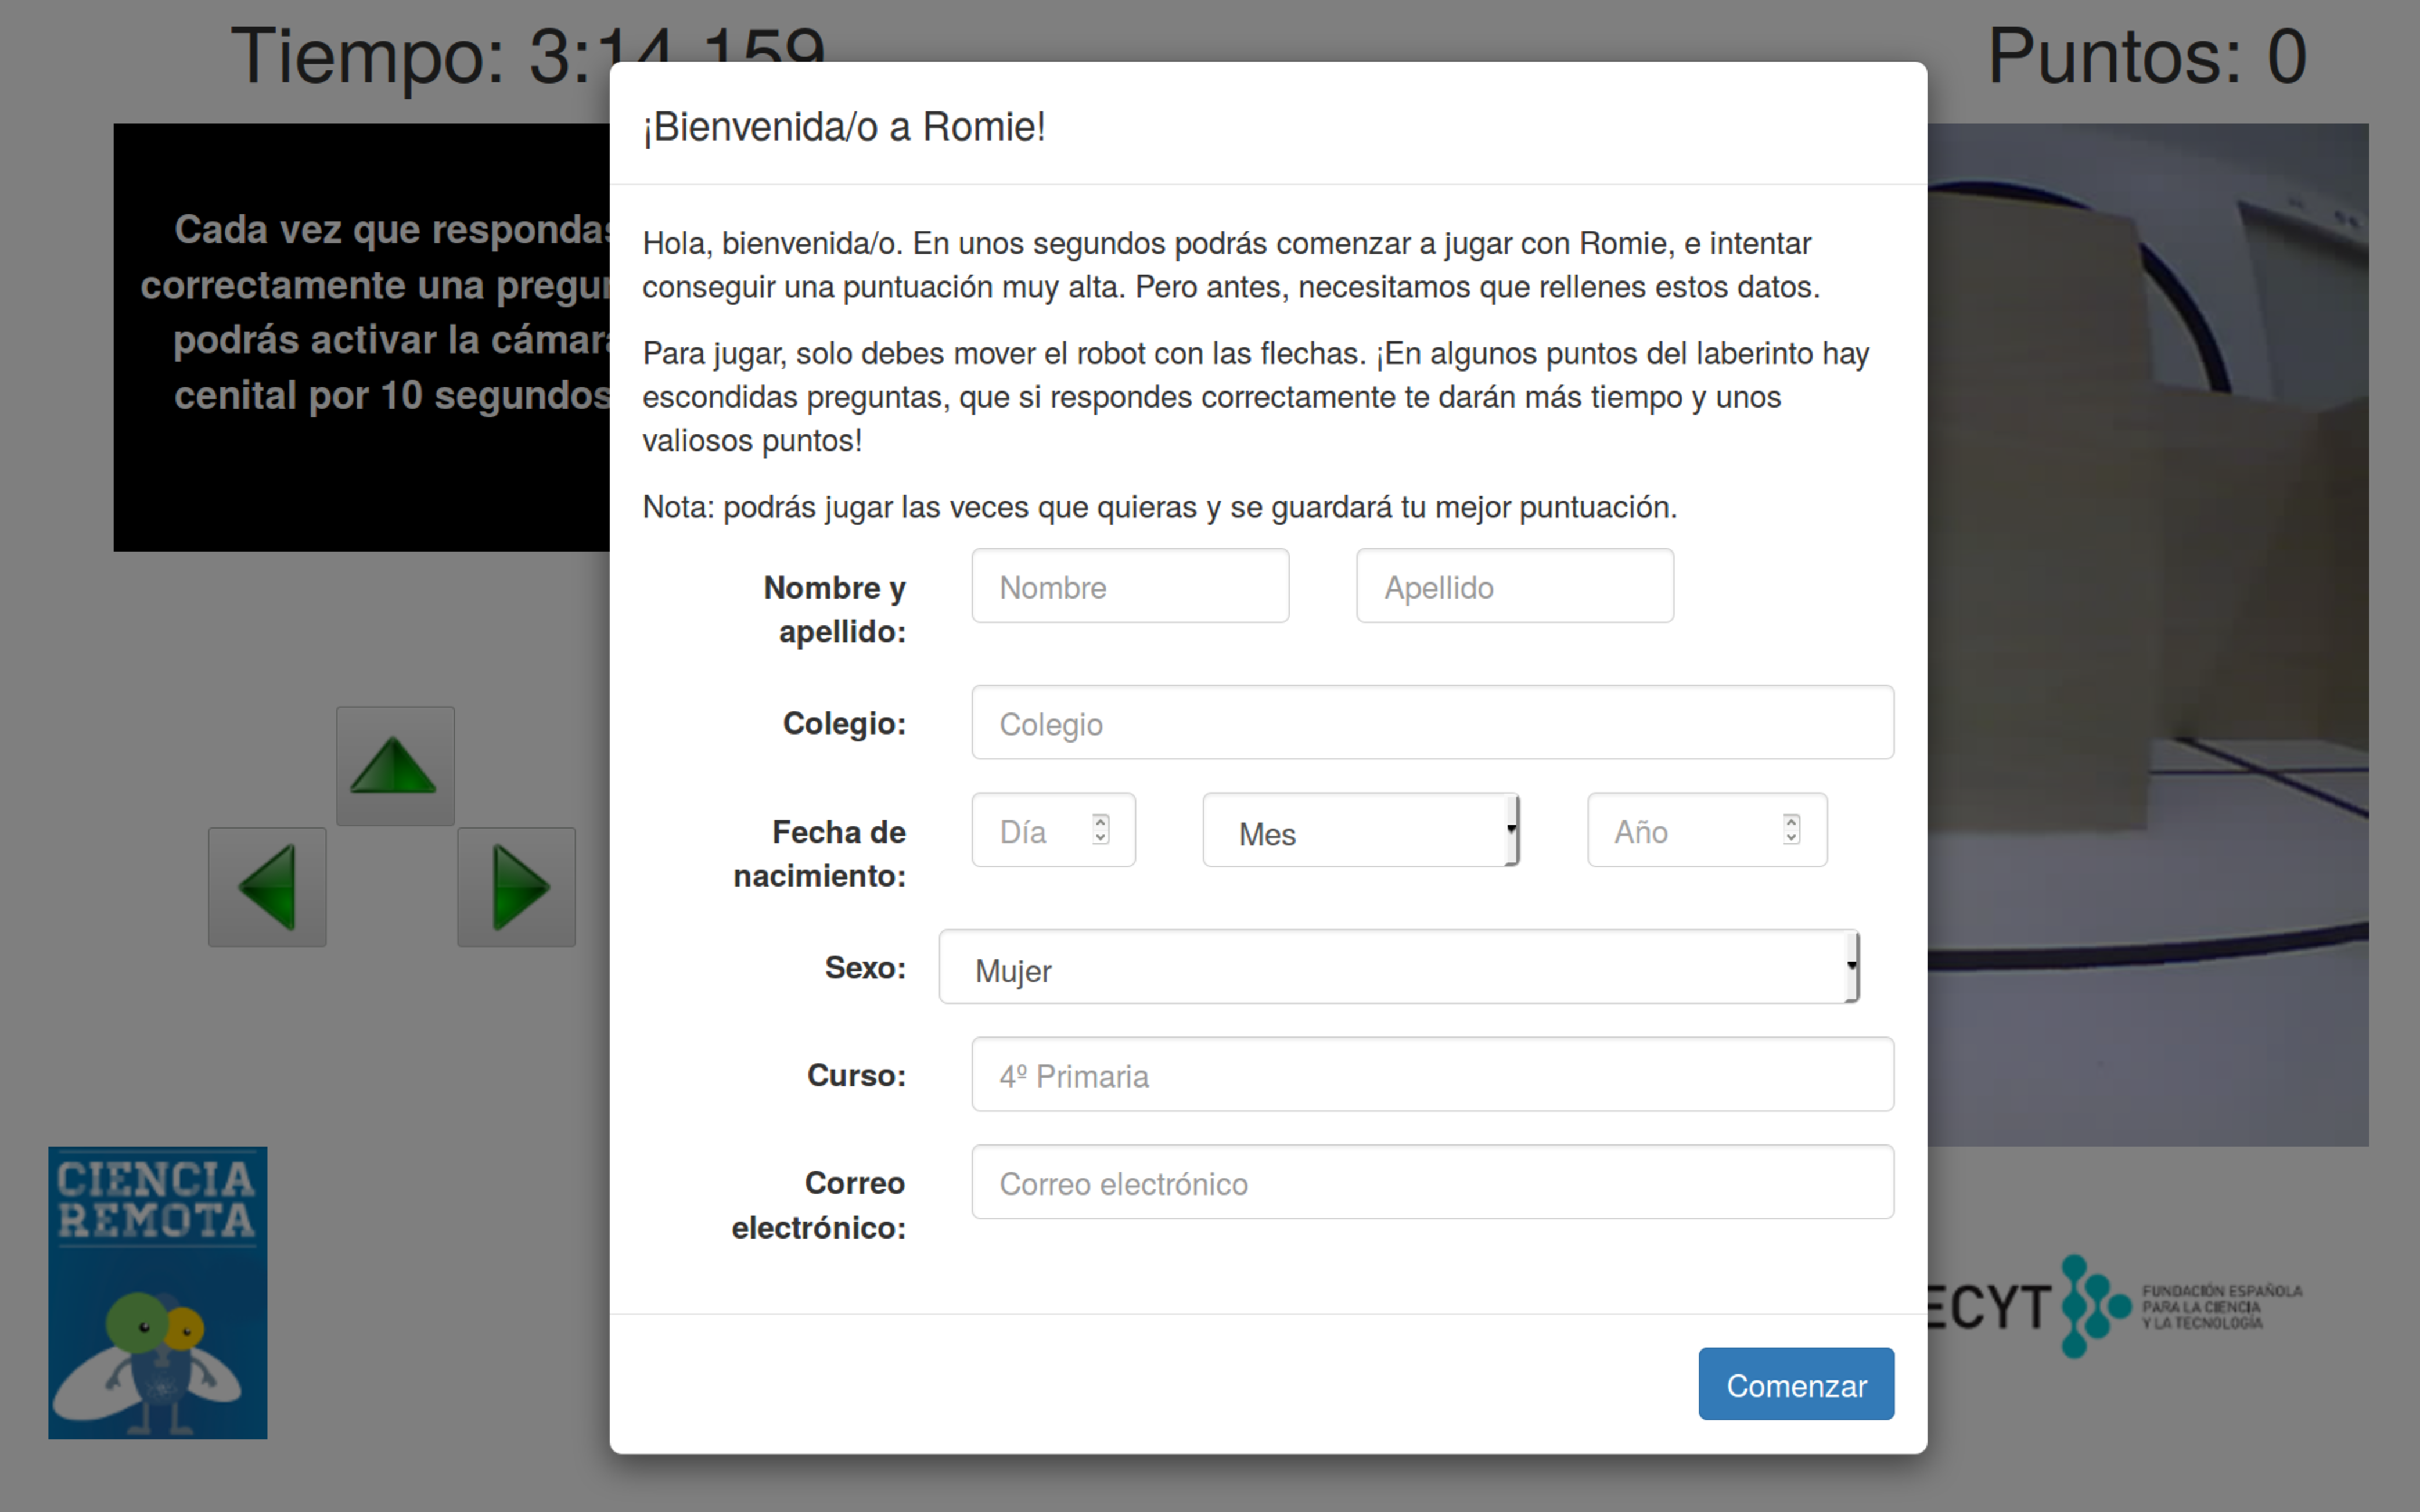
\includegraphics[width=0.85\textwidth]{fig/manuals/trivia/romie-register}
	\caption{Romie's registration form.}
	\label{fig:man:romie_register}
\end{figure}

After the registration, you will be able to play with Romie. The game is pretty easy to use: you
will have three arrows in the left control pad (figure~\ref{fig:man:romie_start}), where you will be
able to click and command the robot to move forward or to turn left or right. Moreover, you will
have the on-board camera to see what the robot does. If you press forward against a wall do not
worry, the robot will not collide.

\begin{figure}[!htbp]
	\centering
	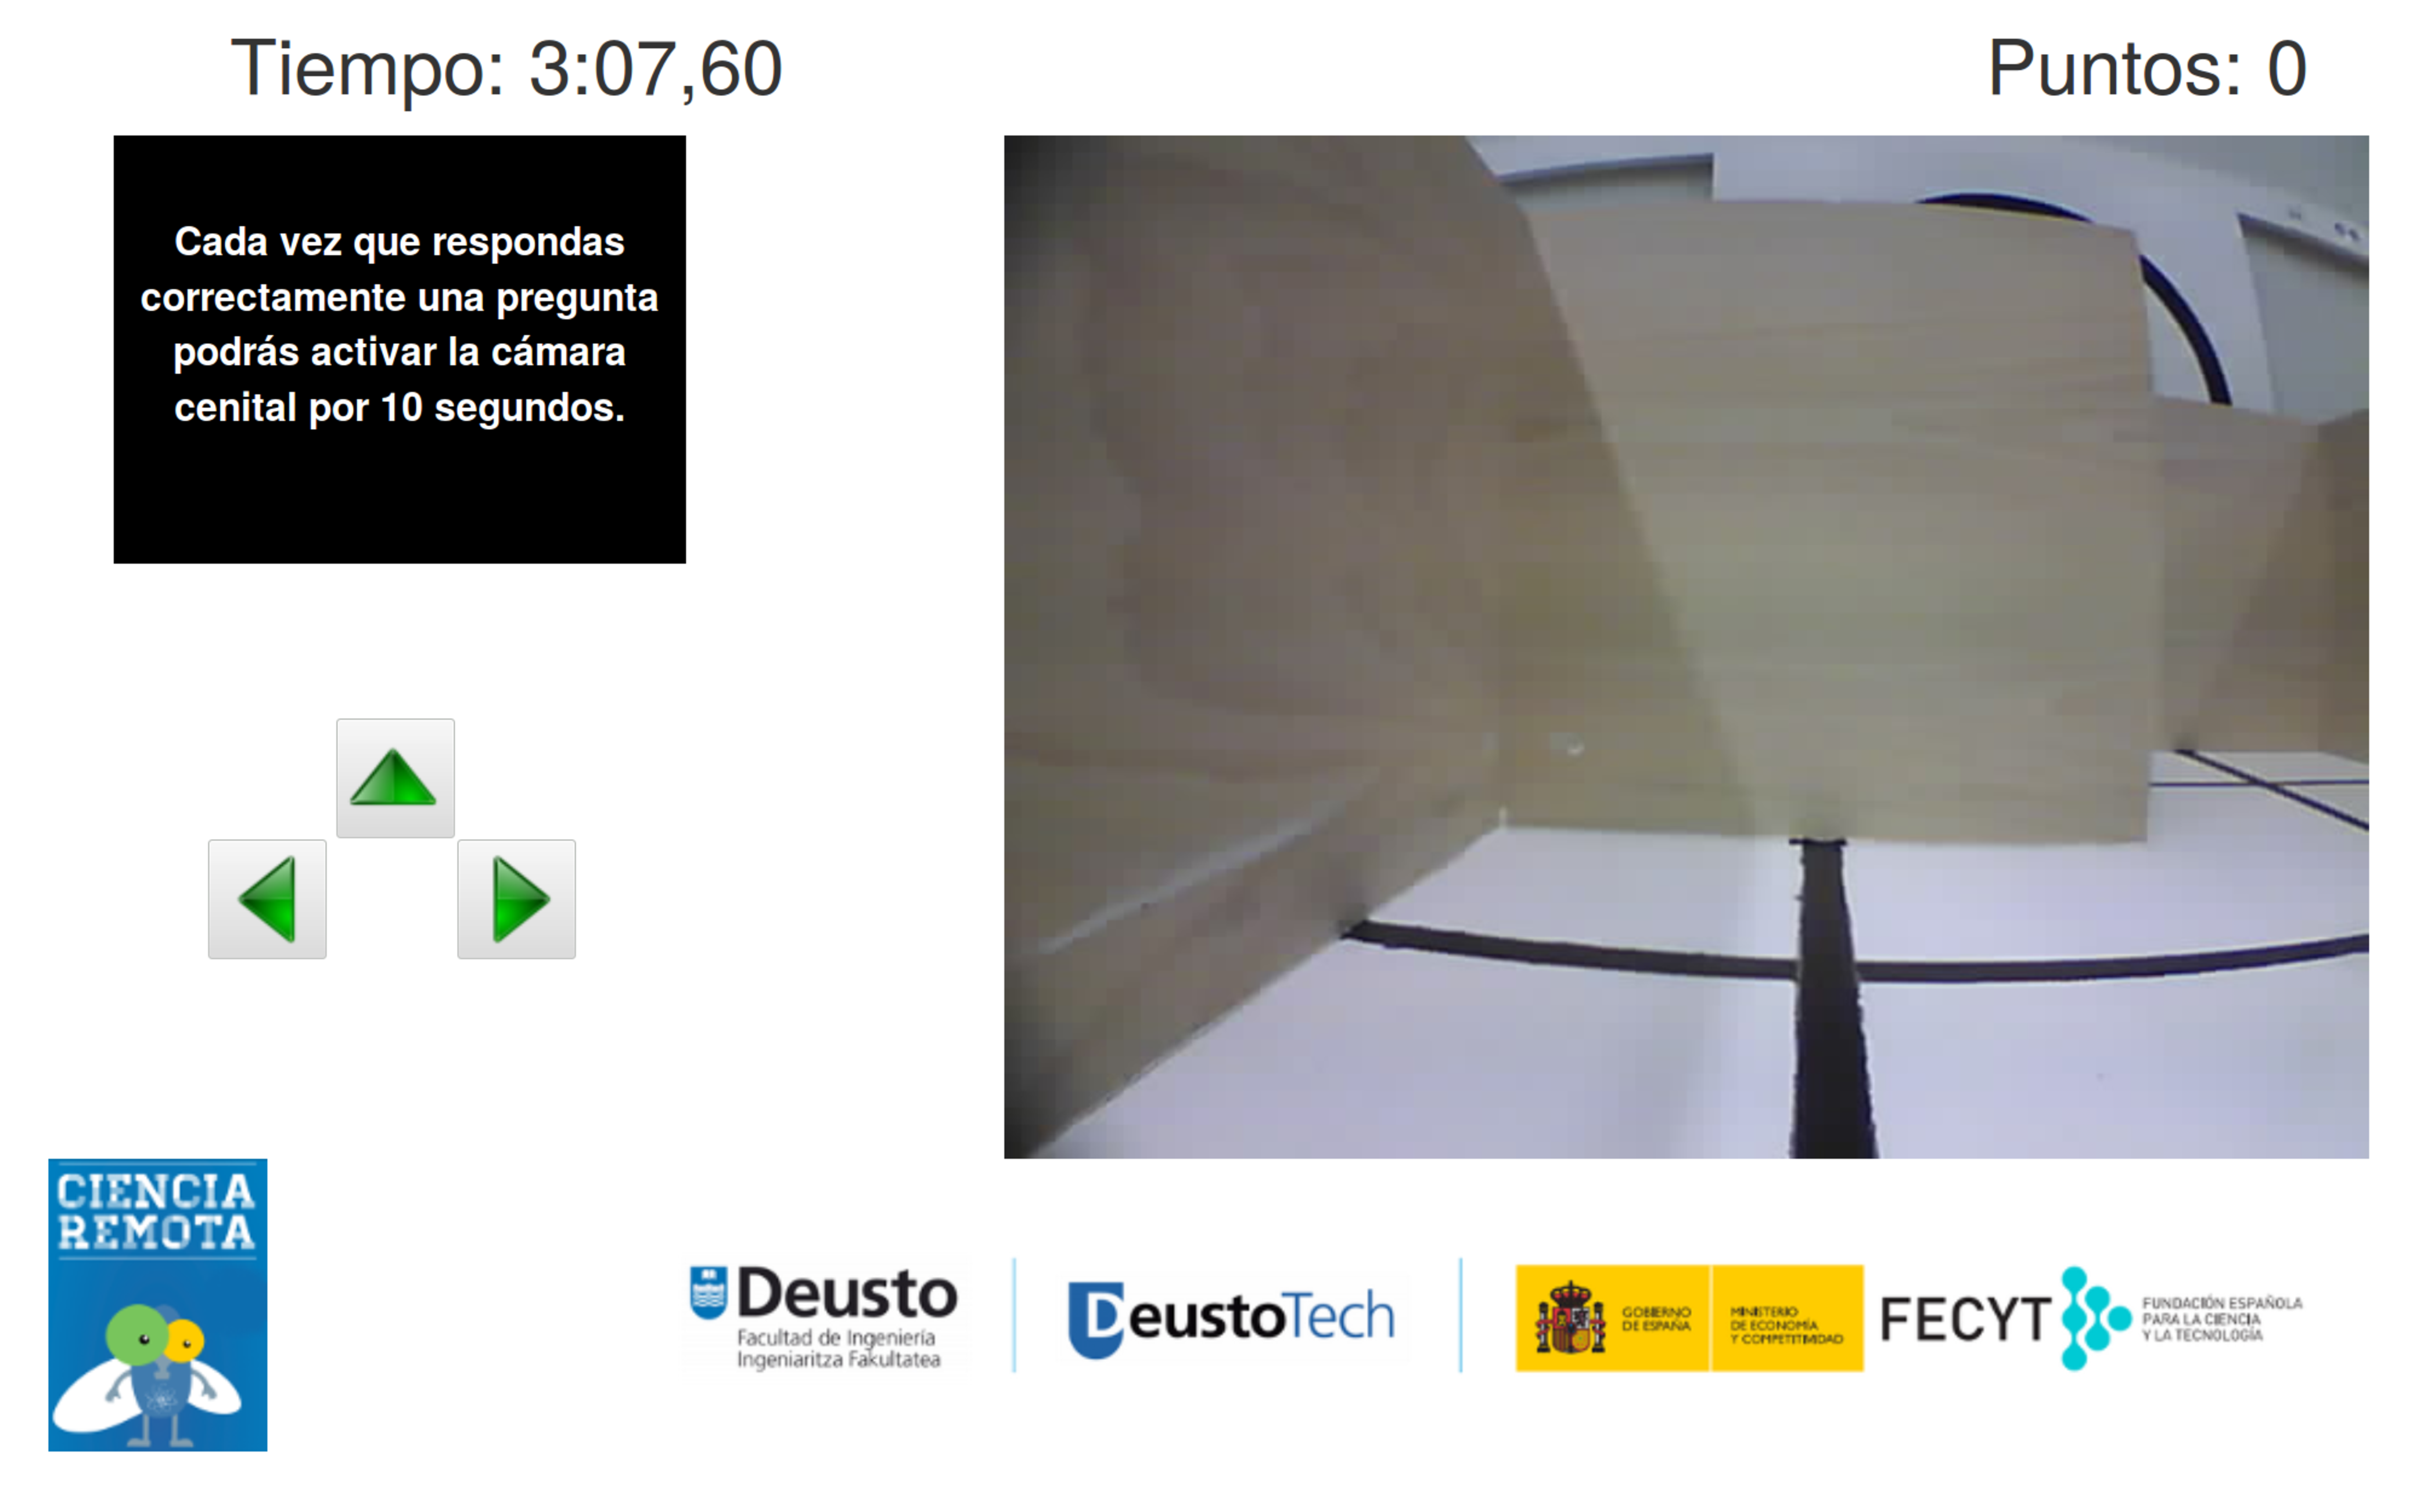
\includegraphics[width=0.85\textwidth]{fig/manuals/trivia/romie-start}
	\caption{Playing with Romie.}
	\label{fig:man:romie_start}
\end{figure}

If you fall in top of a card, you will be asked a question (figure~\ref{fig:man:romie_question}). If
you answer correctly, you will be given points and more time to continue playing. Furthermore, you
will have the opportunity to manually activate the ceiling camera to see all the labyrinth and
decide where to go (figure~\ref{fig:man:romie_ceiling}).

\begin{figure}[!htbp]
	\centering
	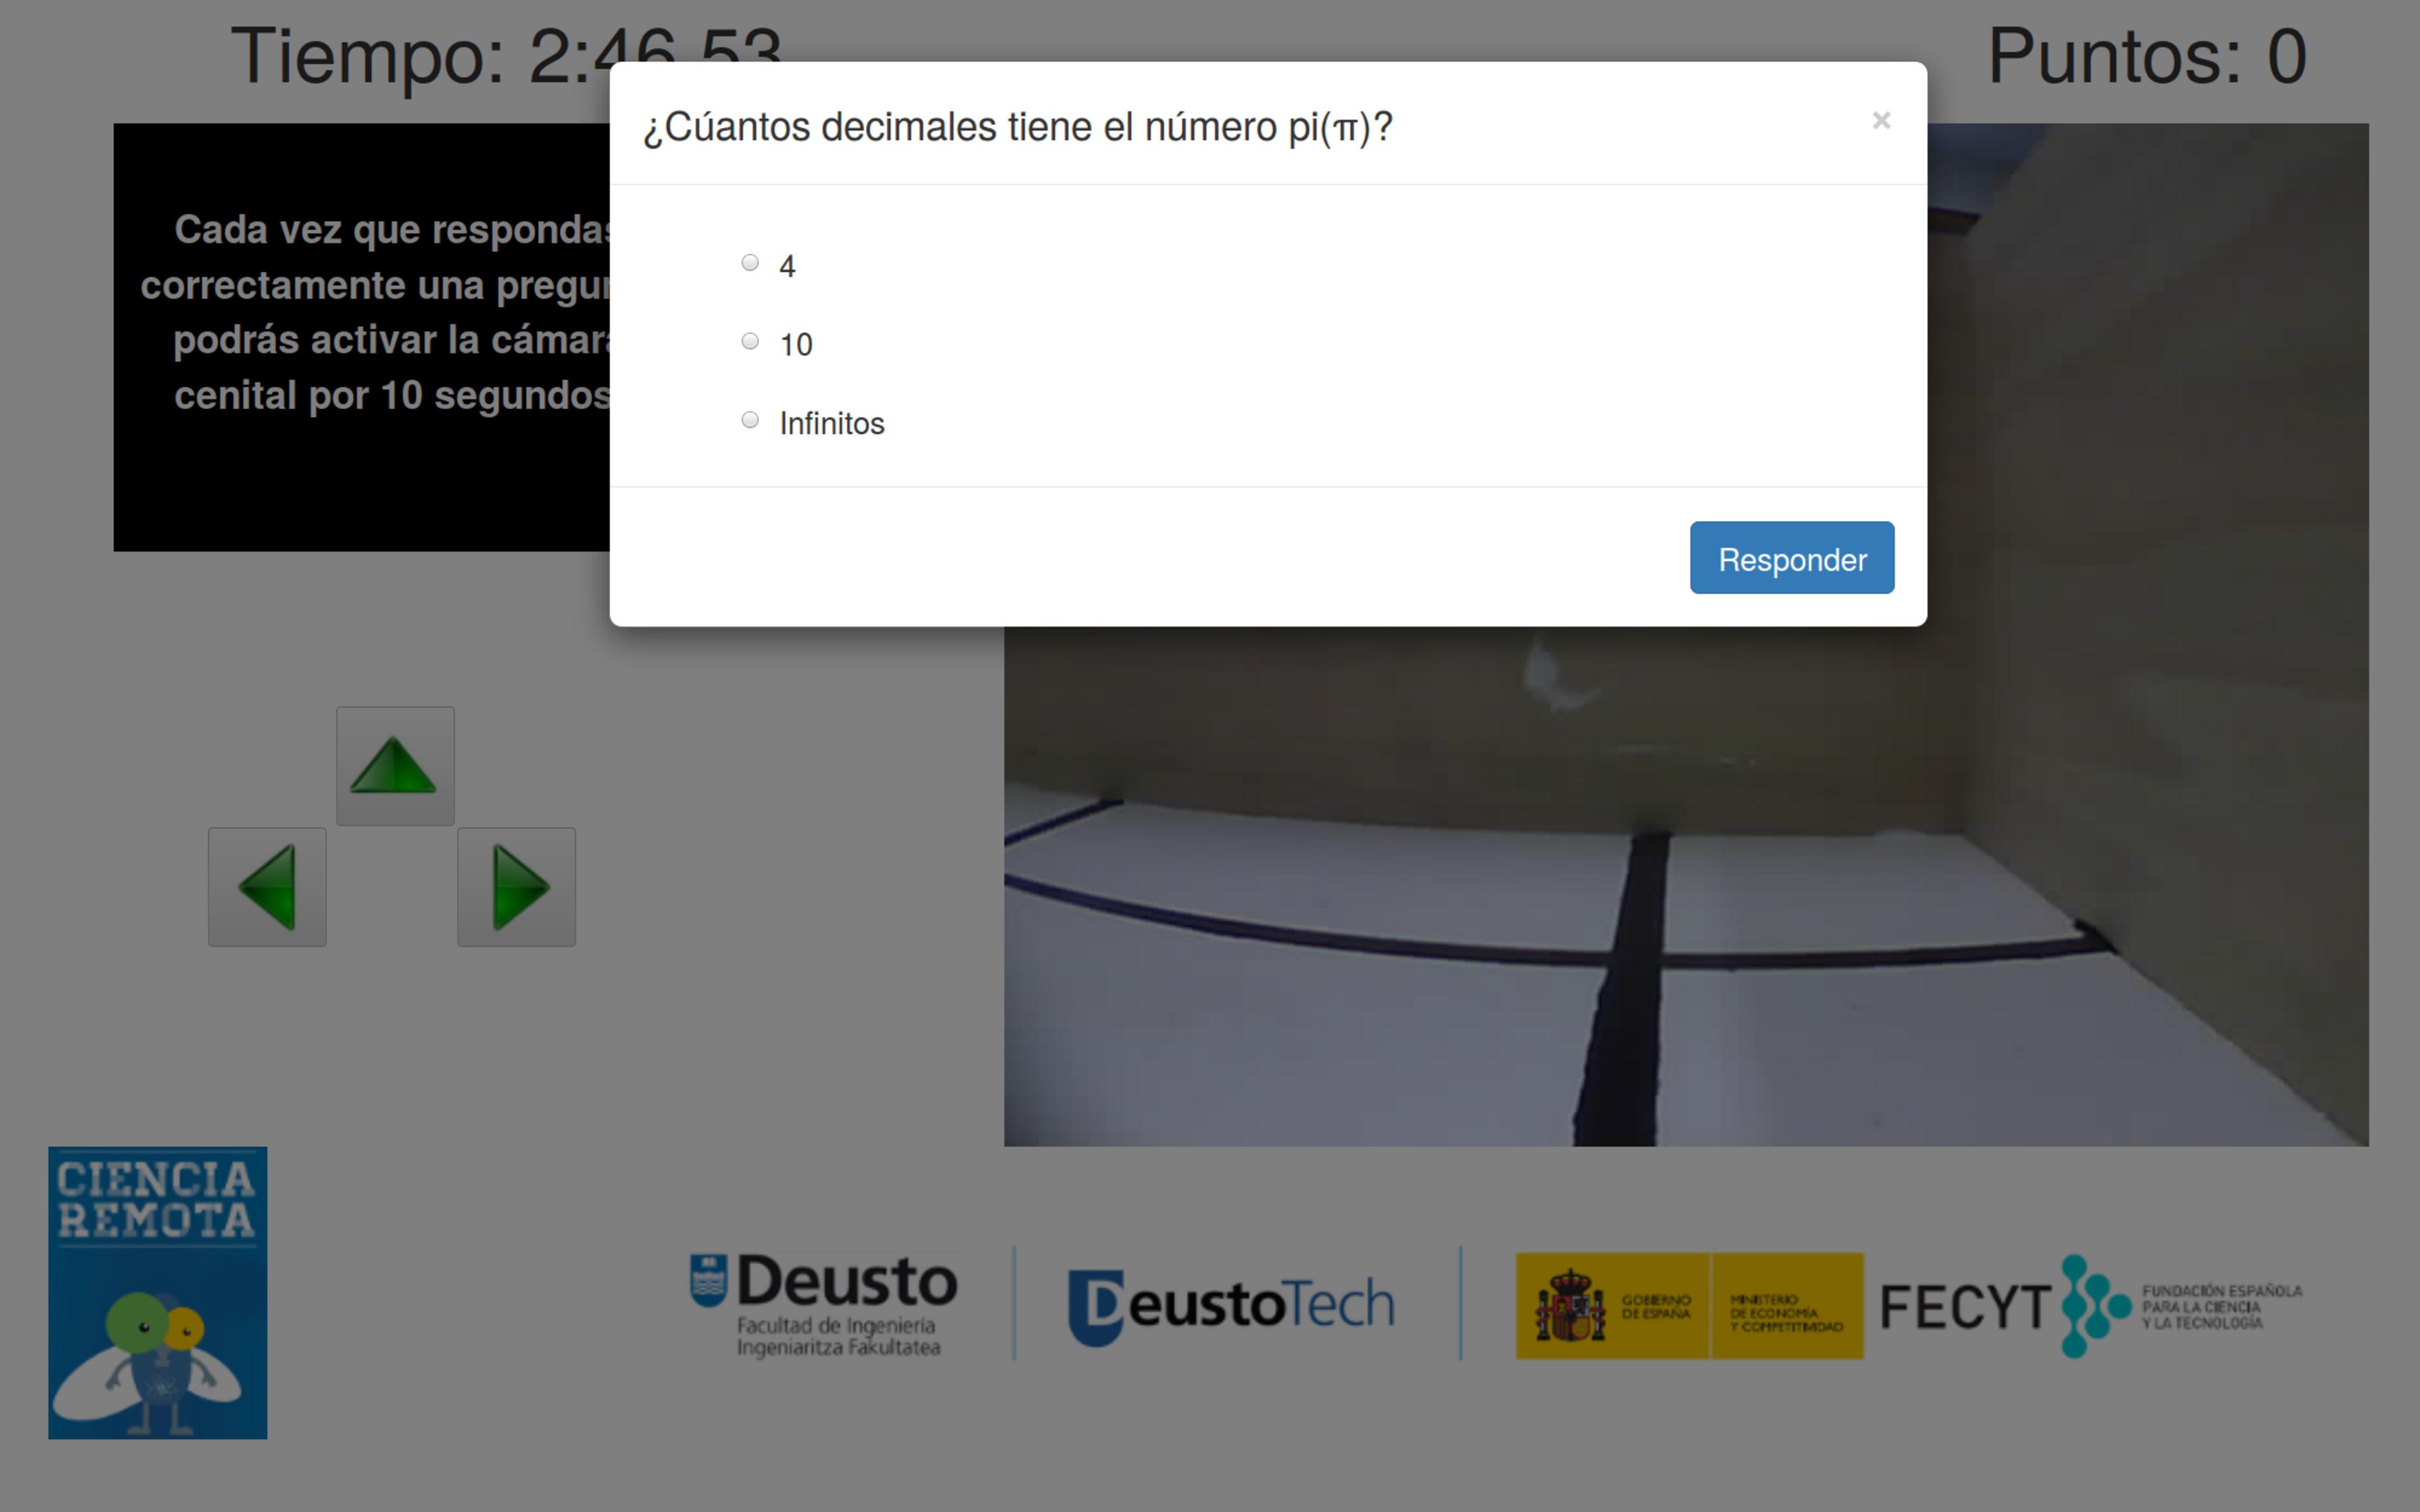
\includegraphics[width=0.85\textwidth]{fig/manuals/trivia/romie-question}
	\caption{Romie asks you questions when you drive onto a card.}
	\label{fig:man:romie_question}
\end{figure}

\begin{figure}[!htbp]
	\centering
	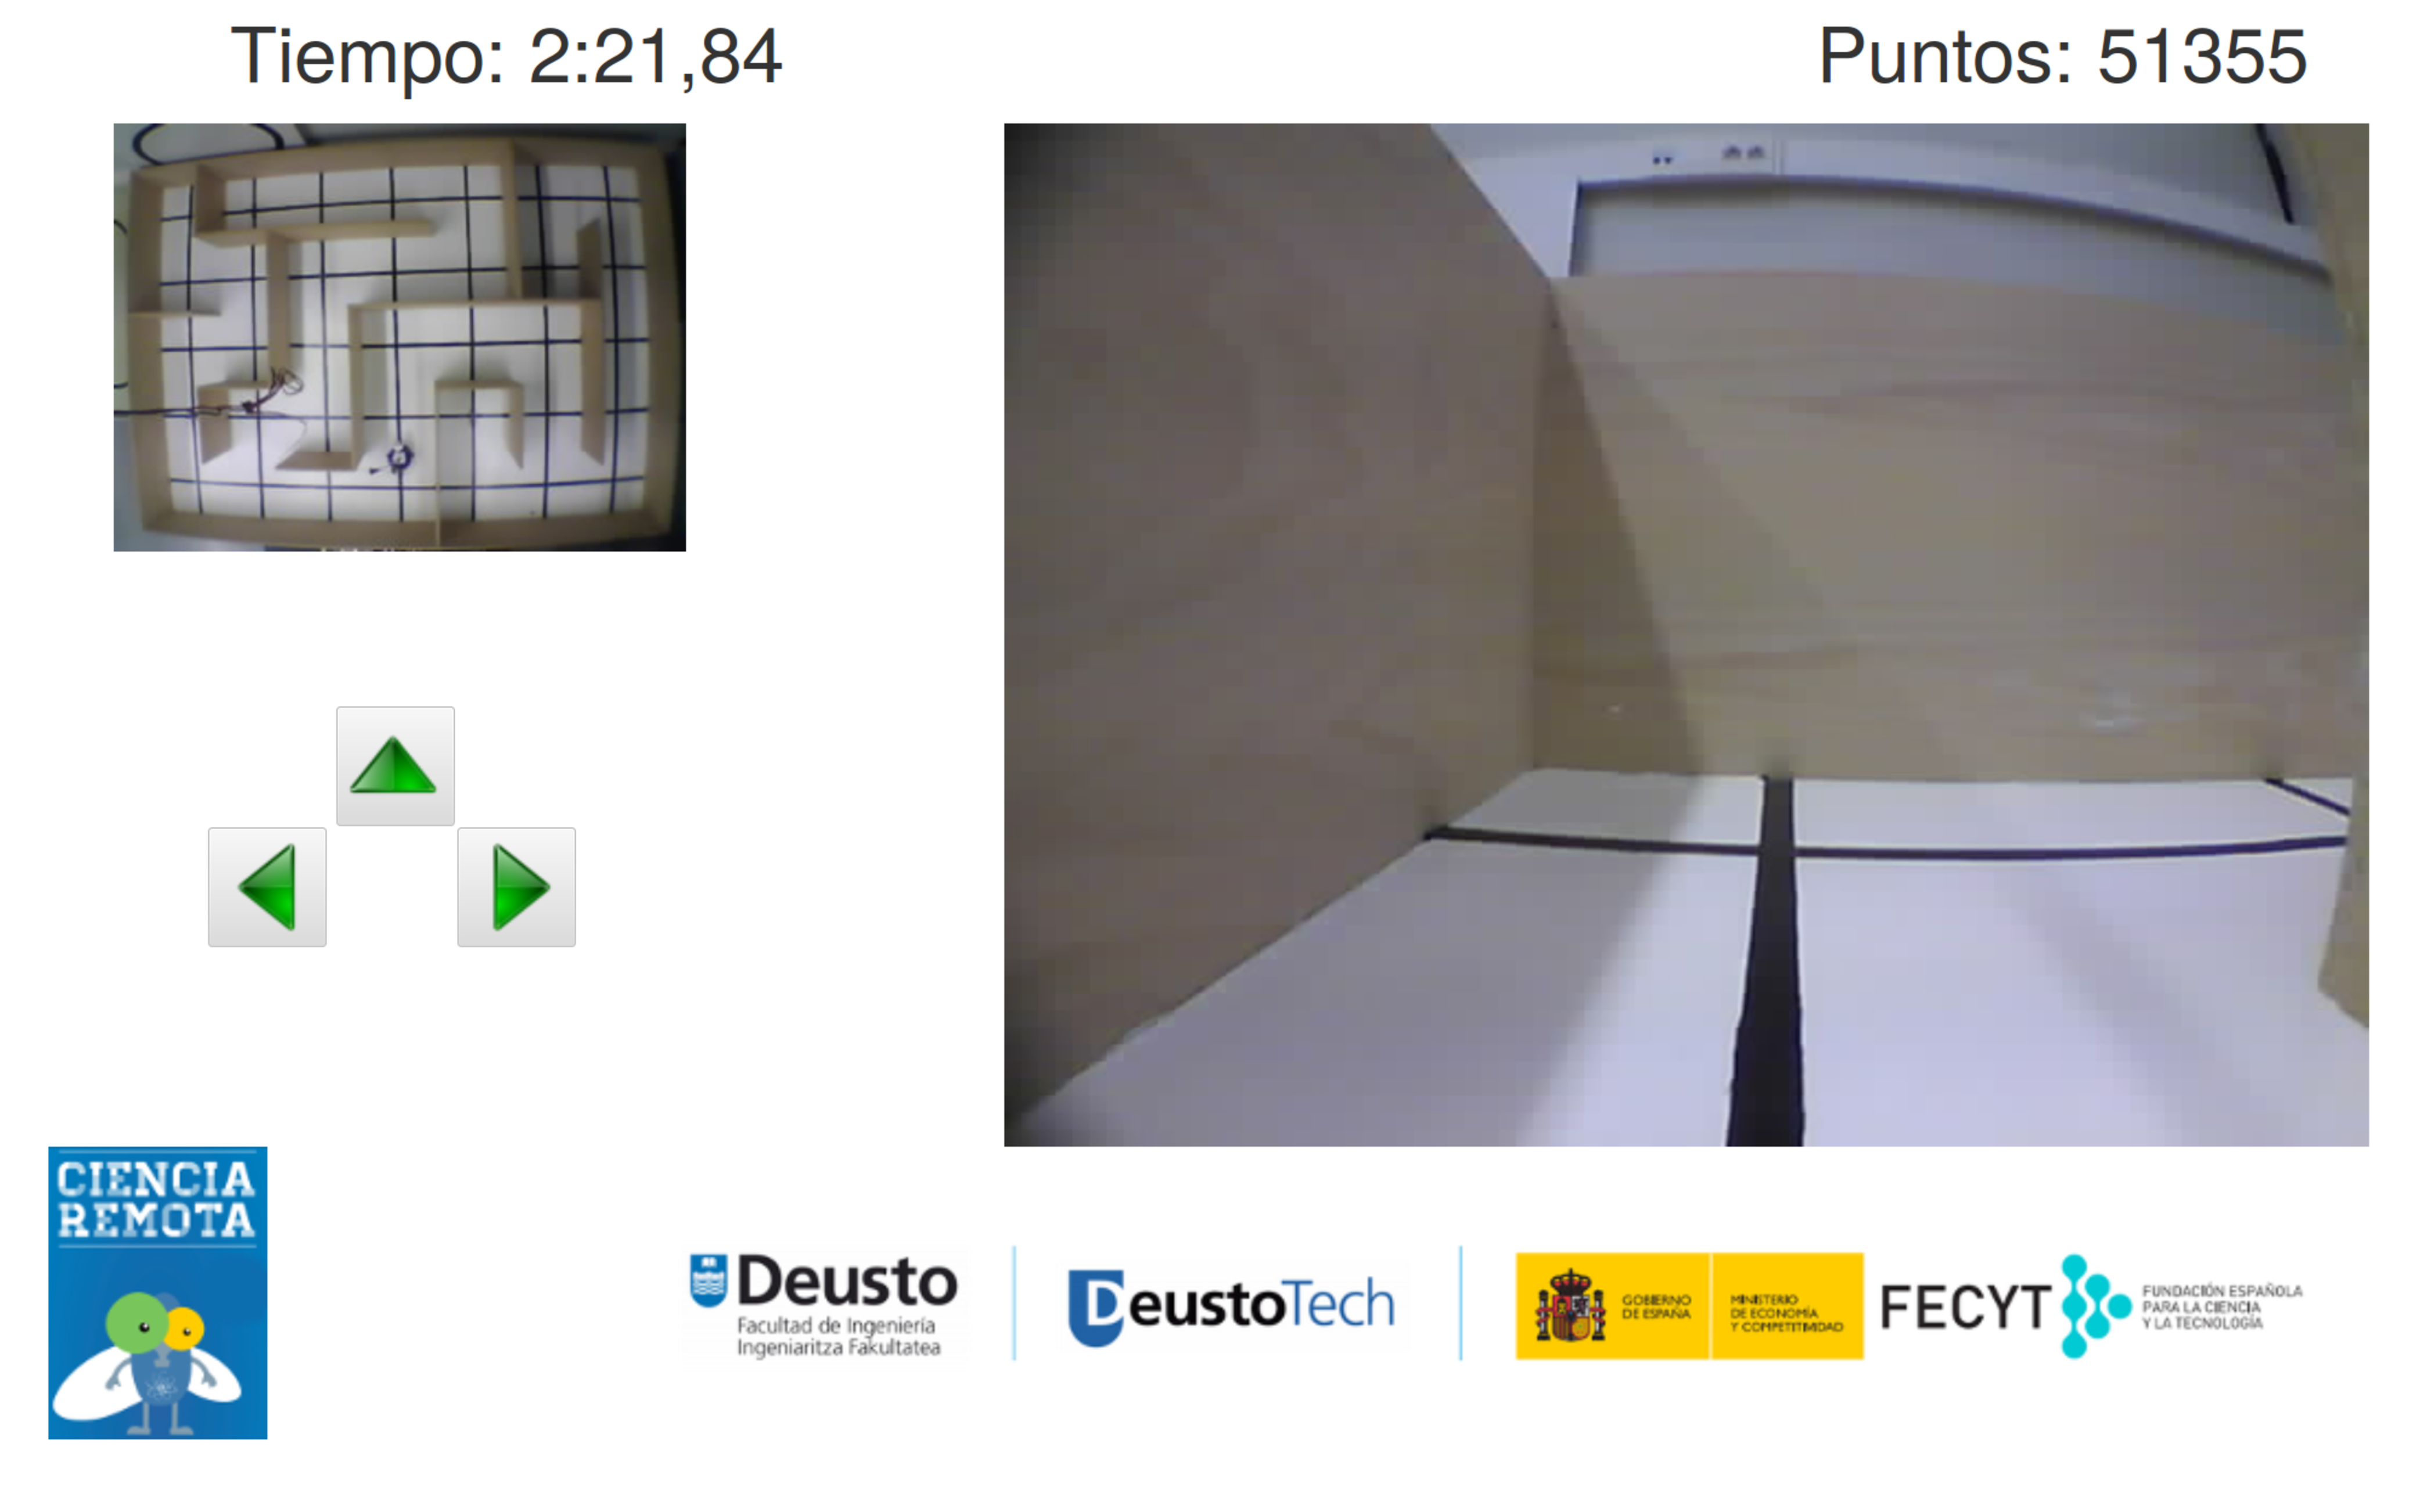
\includegraphics[width=0.85\textwidth]{fig/manuals/trivia/romie-ceiling}
	\caption{You can activate the ceiling camera when you answer a question correctly.}
	\label{fig:man:romie_ceiling}
\end{figure}

Finally, when the time finishes, you will see a ranking with the 10 best scores of the game (less if
there has not been enough users) with your user selected in green if you are in the top ten, as you
can see in figure~\ref{fig:man:romie_ranking}.

\begin{figure}[!htbp]
	\centering
	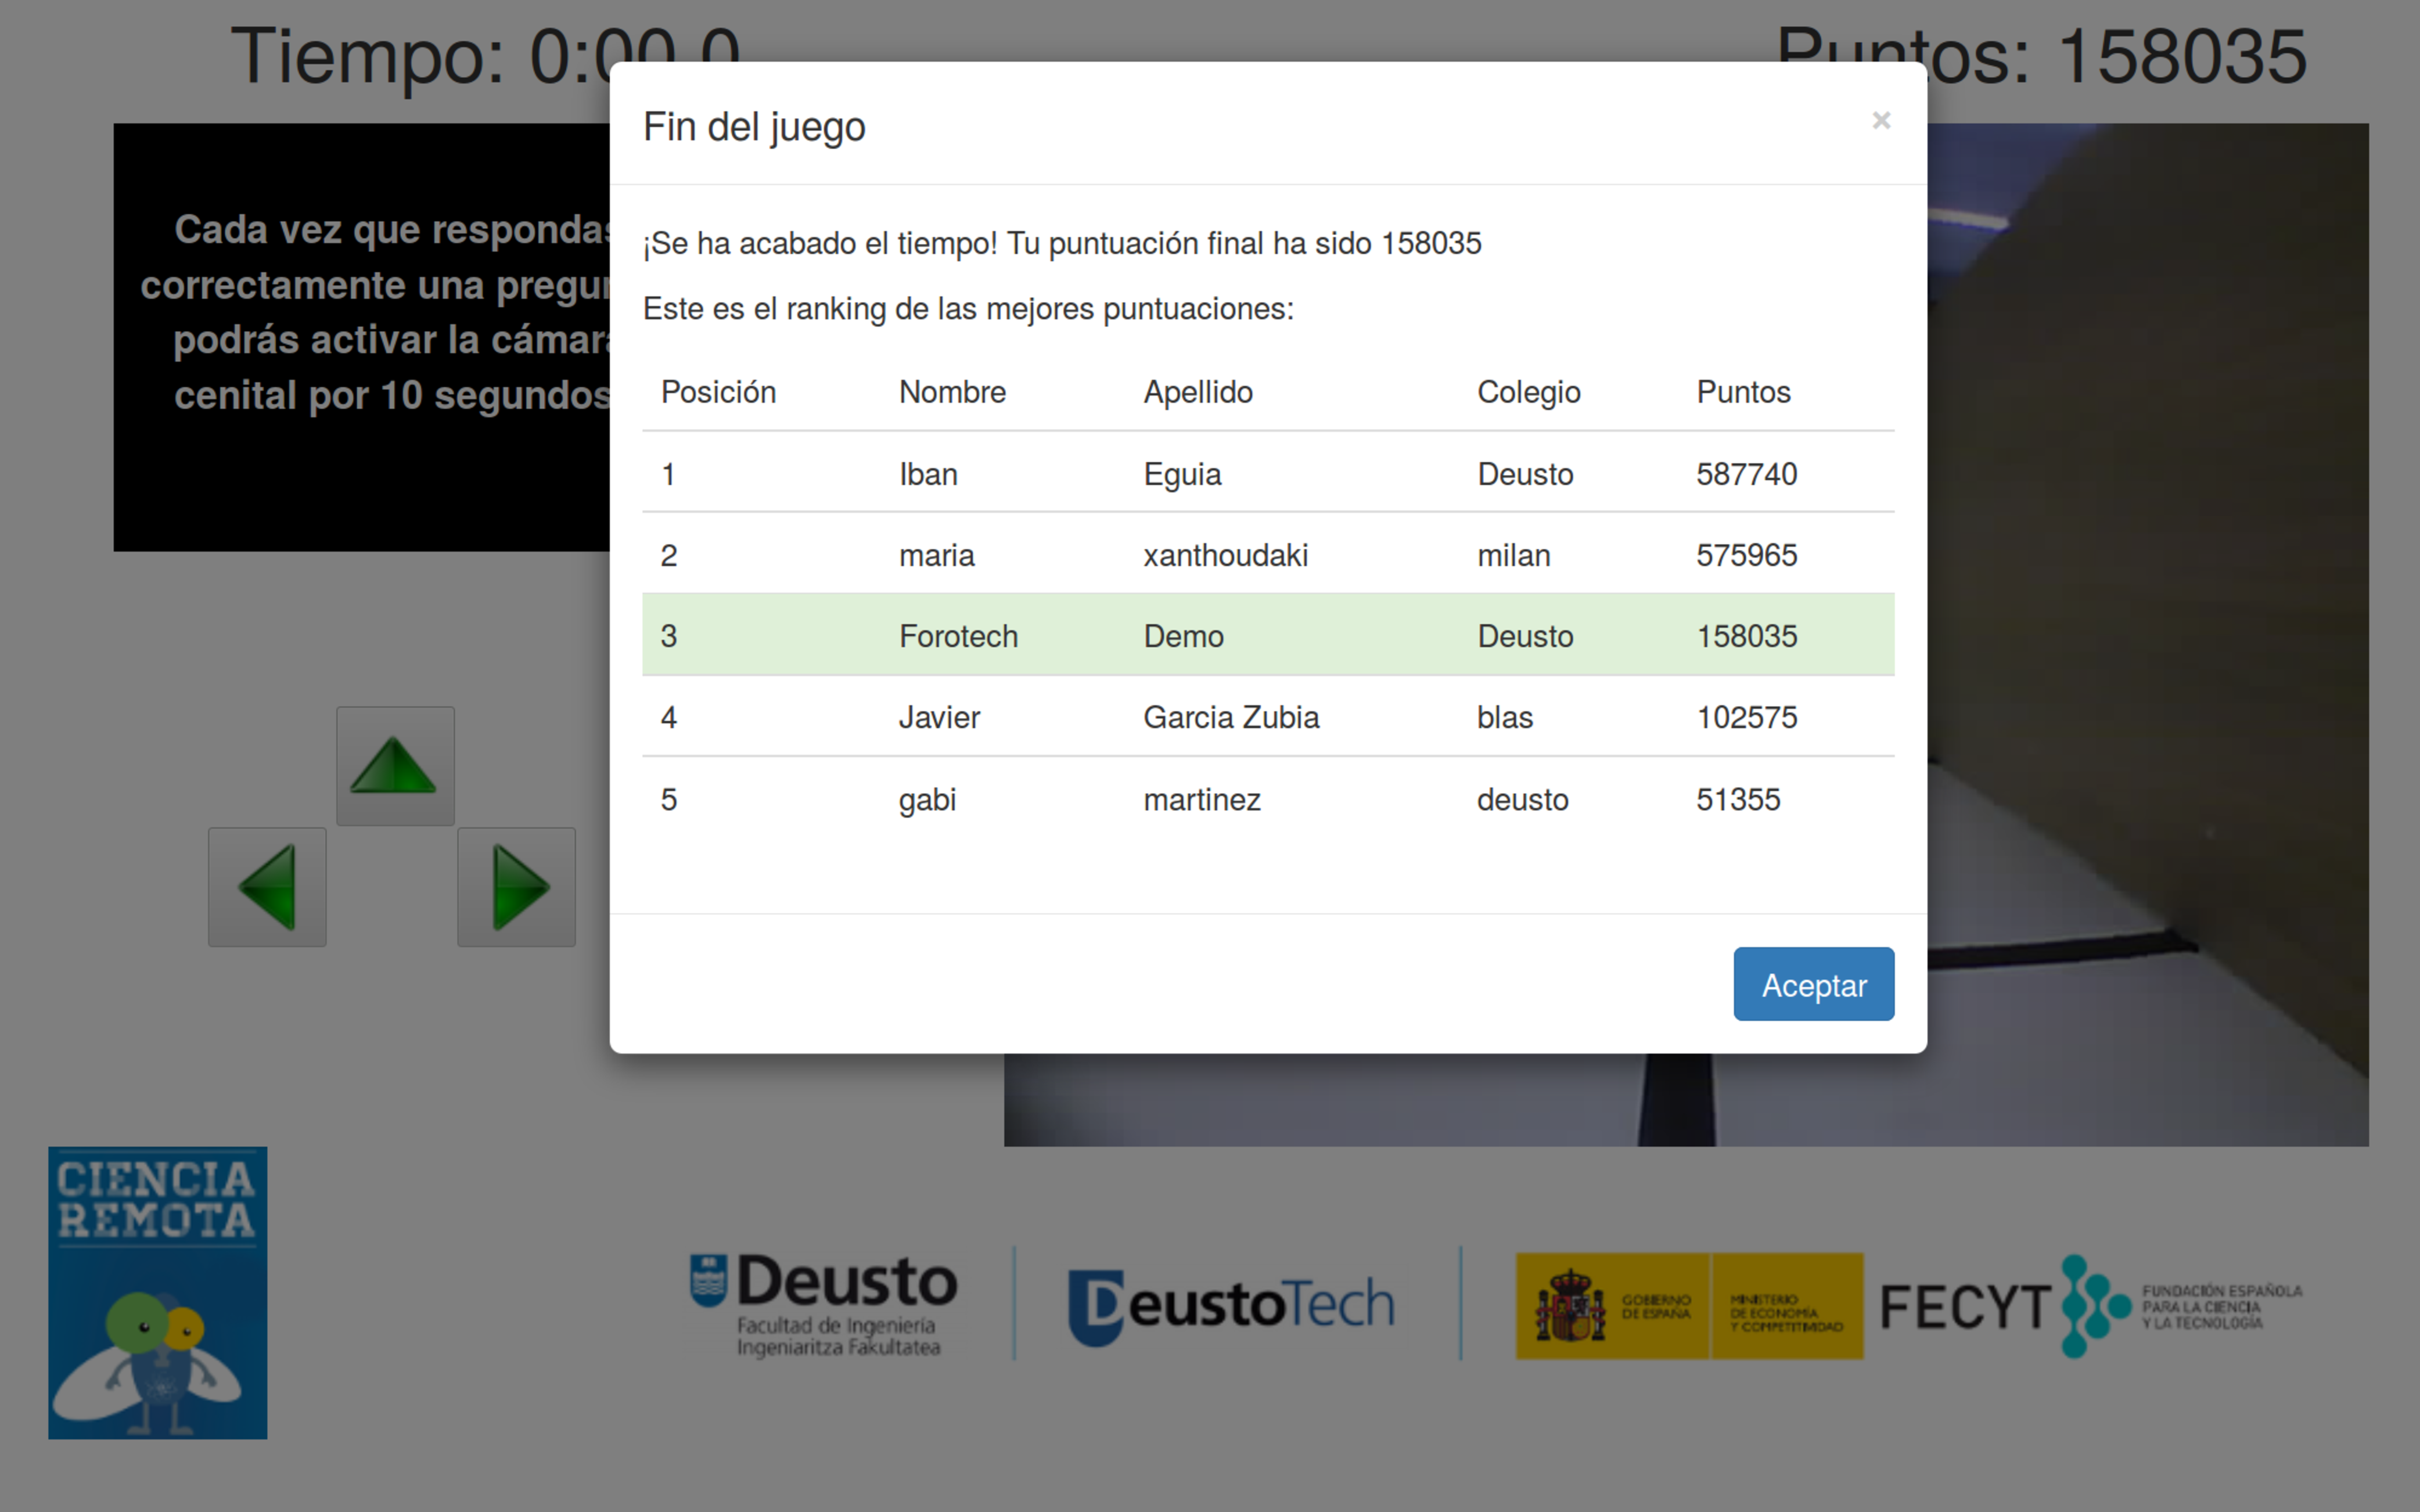
\includegraphics[width=0.85\textwidth]{fig/manuals/trivia/romie-ranking}
	\caption{The final ranking where you can see the best scores.}
	\label{fig:man:romie_ranking}
\end{figure}

\subsection{Issue Management}

During the development we have faced some issues that we have had to deal with. One of the first
issues we had was that the robot was not reading the lines properly, mainly the ones in the
intersections. That was caused because the contrast between the line and the background was
insufficient. We solved it by painting all the labyrinth in white and adding the lines in black
painting them. That way we did not need to use tape and the robot started to work properly.

Other issue we found was that the robot did not read the \acrshort{rfid} tags every time it went on
top of them. The problem was that the \acrshort{rfid} reader we were using, the ID-12 seemed to have
some working issues, since the reader was located about 10-15~mm from the floor. We decided to
change it by a ID-20 reader, that has a 180~mm range~\cite{rfid} and worked perfectly.

Furthermore, we had the problem with electricity, that it was using batteries, and as we have seen
above, we had to change it to cables. The main issue was that the cables would get entangled with
the walls. We solved it by extending a flexible artifact in top of the robot
(figure~\ref{fig:lines}).

\begin{figure}[!htbp]
	\centering
	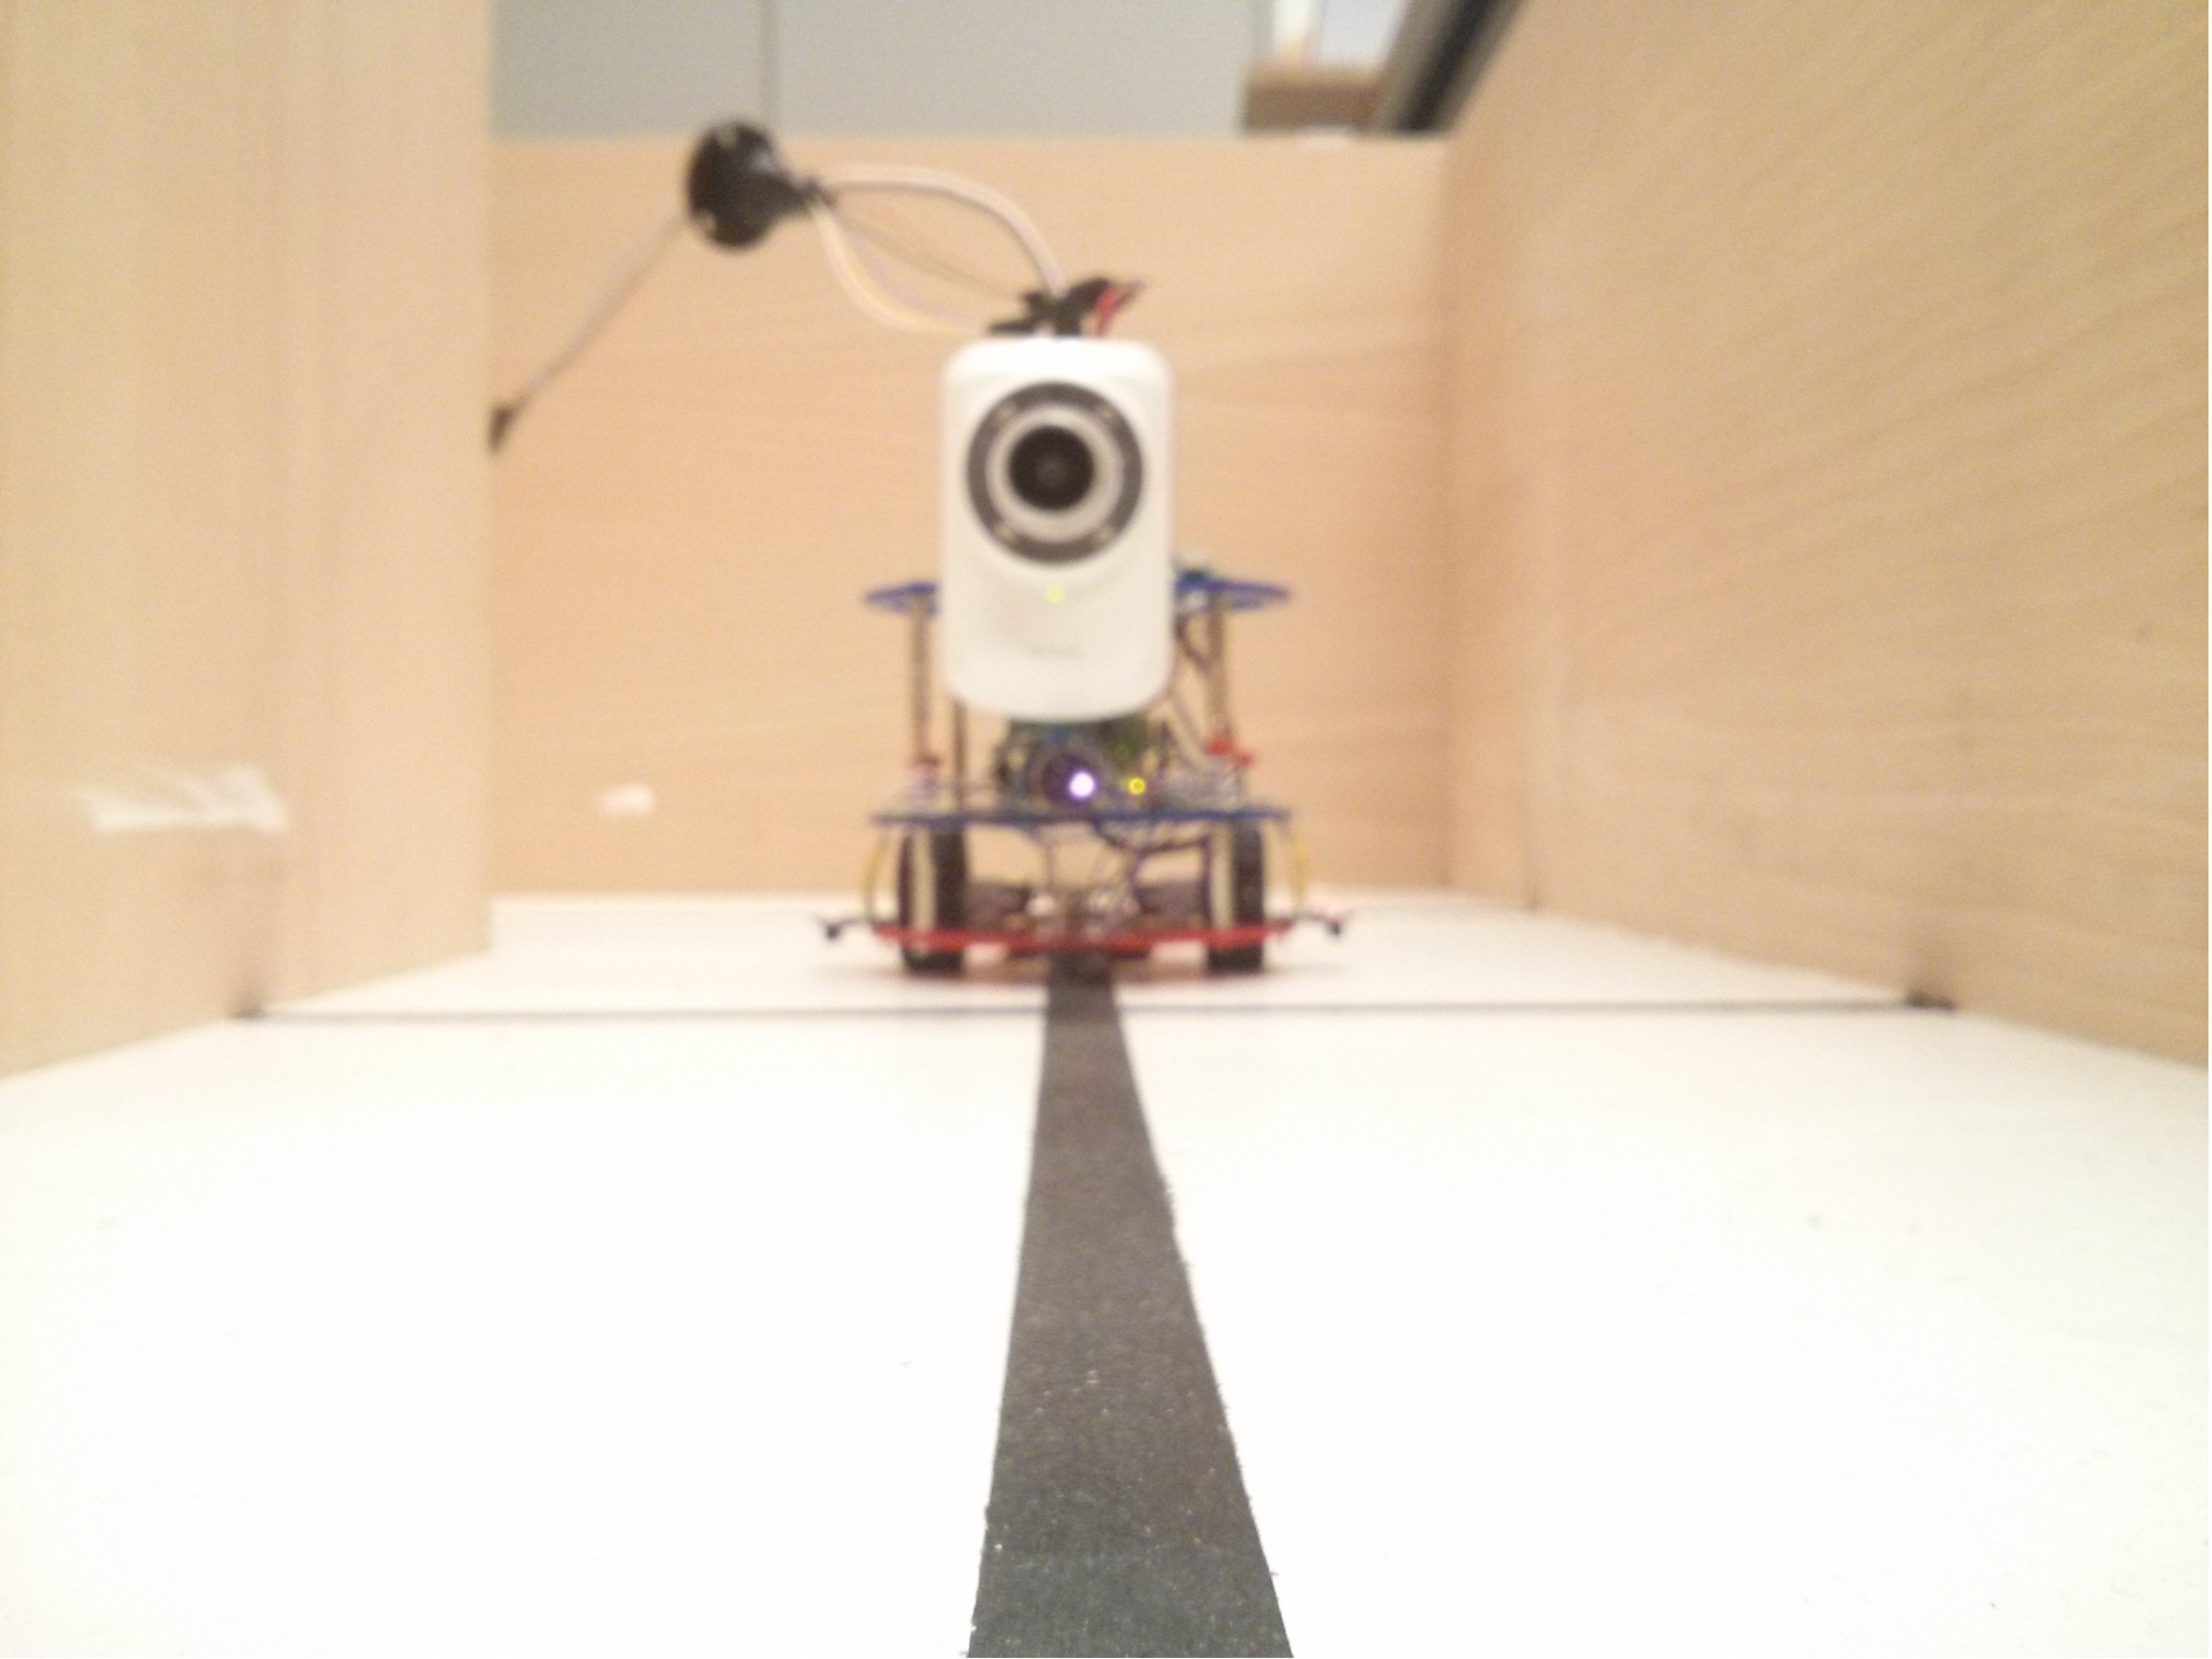
\includegraphics[height=0.35\textheight]{fig/lines}
	\caption{Romie must not get entangled with the walls.}
	\label{fig:lines}
\end{figure}

Finally, we had a problem with the wall sensor, since it would disconnect sometimes. This was a
hardware issue that we could not solve easily, since the sensor would arrive at least 1 month after
being requested. Taking that into account we decided to implement a software solution directly in
the robot so that it would go back automatically if something went wrong, as we can see in
algorithm~\ref{alg:romie_wall}.

\begin{center}
\begin{minipage}{.9\textwidth}
\singlespace
\begin{pyglist}[language=c, caption={Arduino code for returning if wall was hit.},
	label={alg:romie_wall}, listingname={Algorithm}, numbers=left]
if (millis()-lastTimeFollow >= 8000) {
	while(digitalRead(FLIline) == HIGH) Motors.turnRight(100);
	while(digitalRead(FRIline) == LOW) Motors.turnRight(100);
	FollowLine();
	lastTimeFollow=millis();
}
\end{pyglist}
\end{minipage}
\end{center}


\section{Labpsico Experiment Integration}

When we were finishing the trivial type game,...

TODO: Labpsico experiment

\subsection{Software Requirements}

\subsection{Design Specification}

\subsection{Deployment Considerations}

\subsection{Testing Plan}

\subsection{User Manual}

\subsection{Issue Management}


\clearpage
\section{Visual Programming}

TODO: Visual Programming

\subsection{Software Requirements}

\subsection{Design Specification}

\subsection{Deployment Considerations}

\subsection{Testing Plan}

\subsection{User Manual}

\subsection{Issue Management}


\chapter{Conclusions and Future Work}

In this project a complete platform has been developed and its value has been demonstrated by
testing it with real users and by developing two services using the platform. Therefore, here can be
found the conclusions of this development, preceded with the usage statistics of the project, one of
the objectives of the project itself.

\section{Usage Statistics}

This project was tested during the Deusto's ForoTech engineering week (figure~\ref{fig:forotech}).
During that testing that lasted for 8 days, hundreds of students saw the system. There was a live
demo in the forum itself, where students learned how to play the game and received their own user
and password to play from home. During those demonstrations, the experiment was used 72 times, with
a total of 16,119.5 seconds of use (about 4 hours and a half).

\begin{figure}[ht]
	\centering
	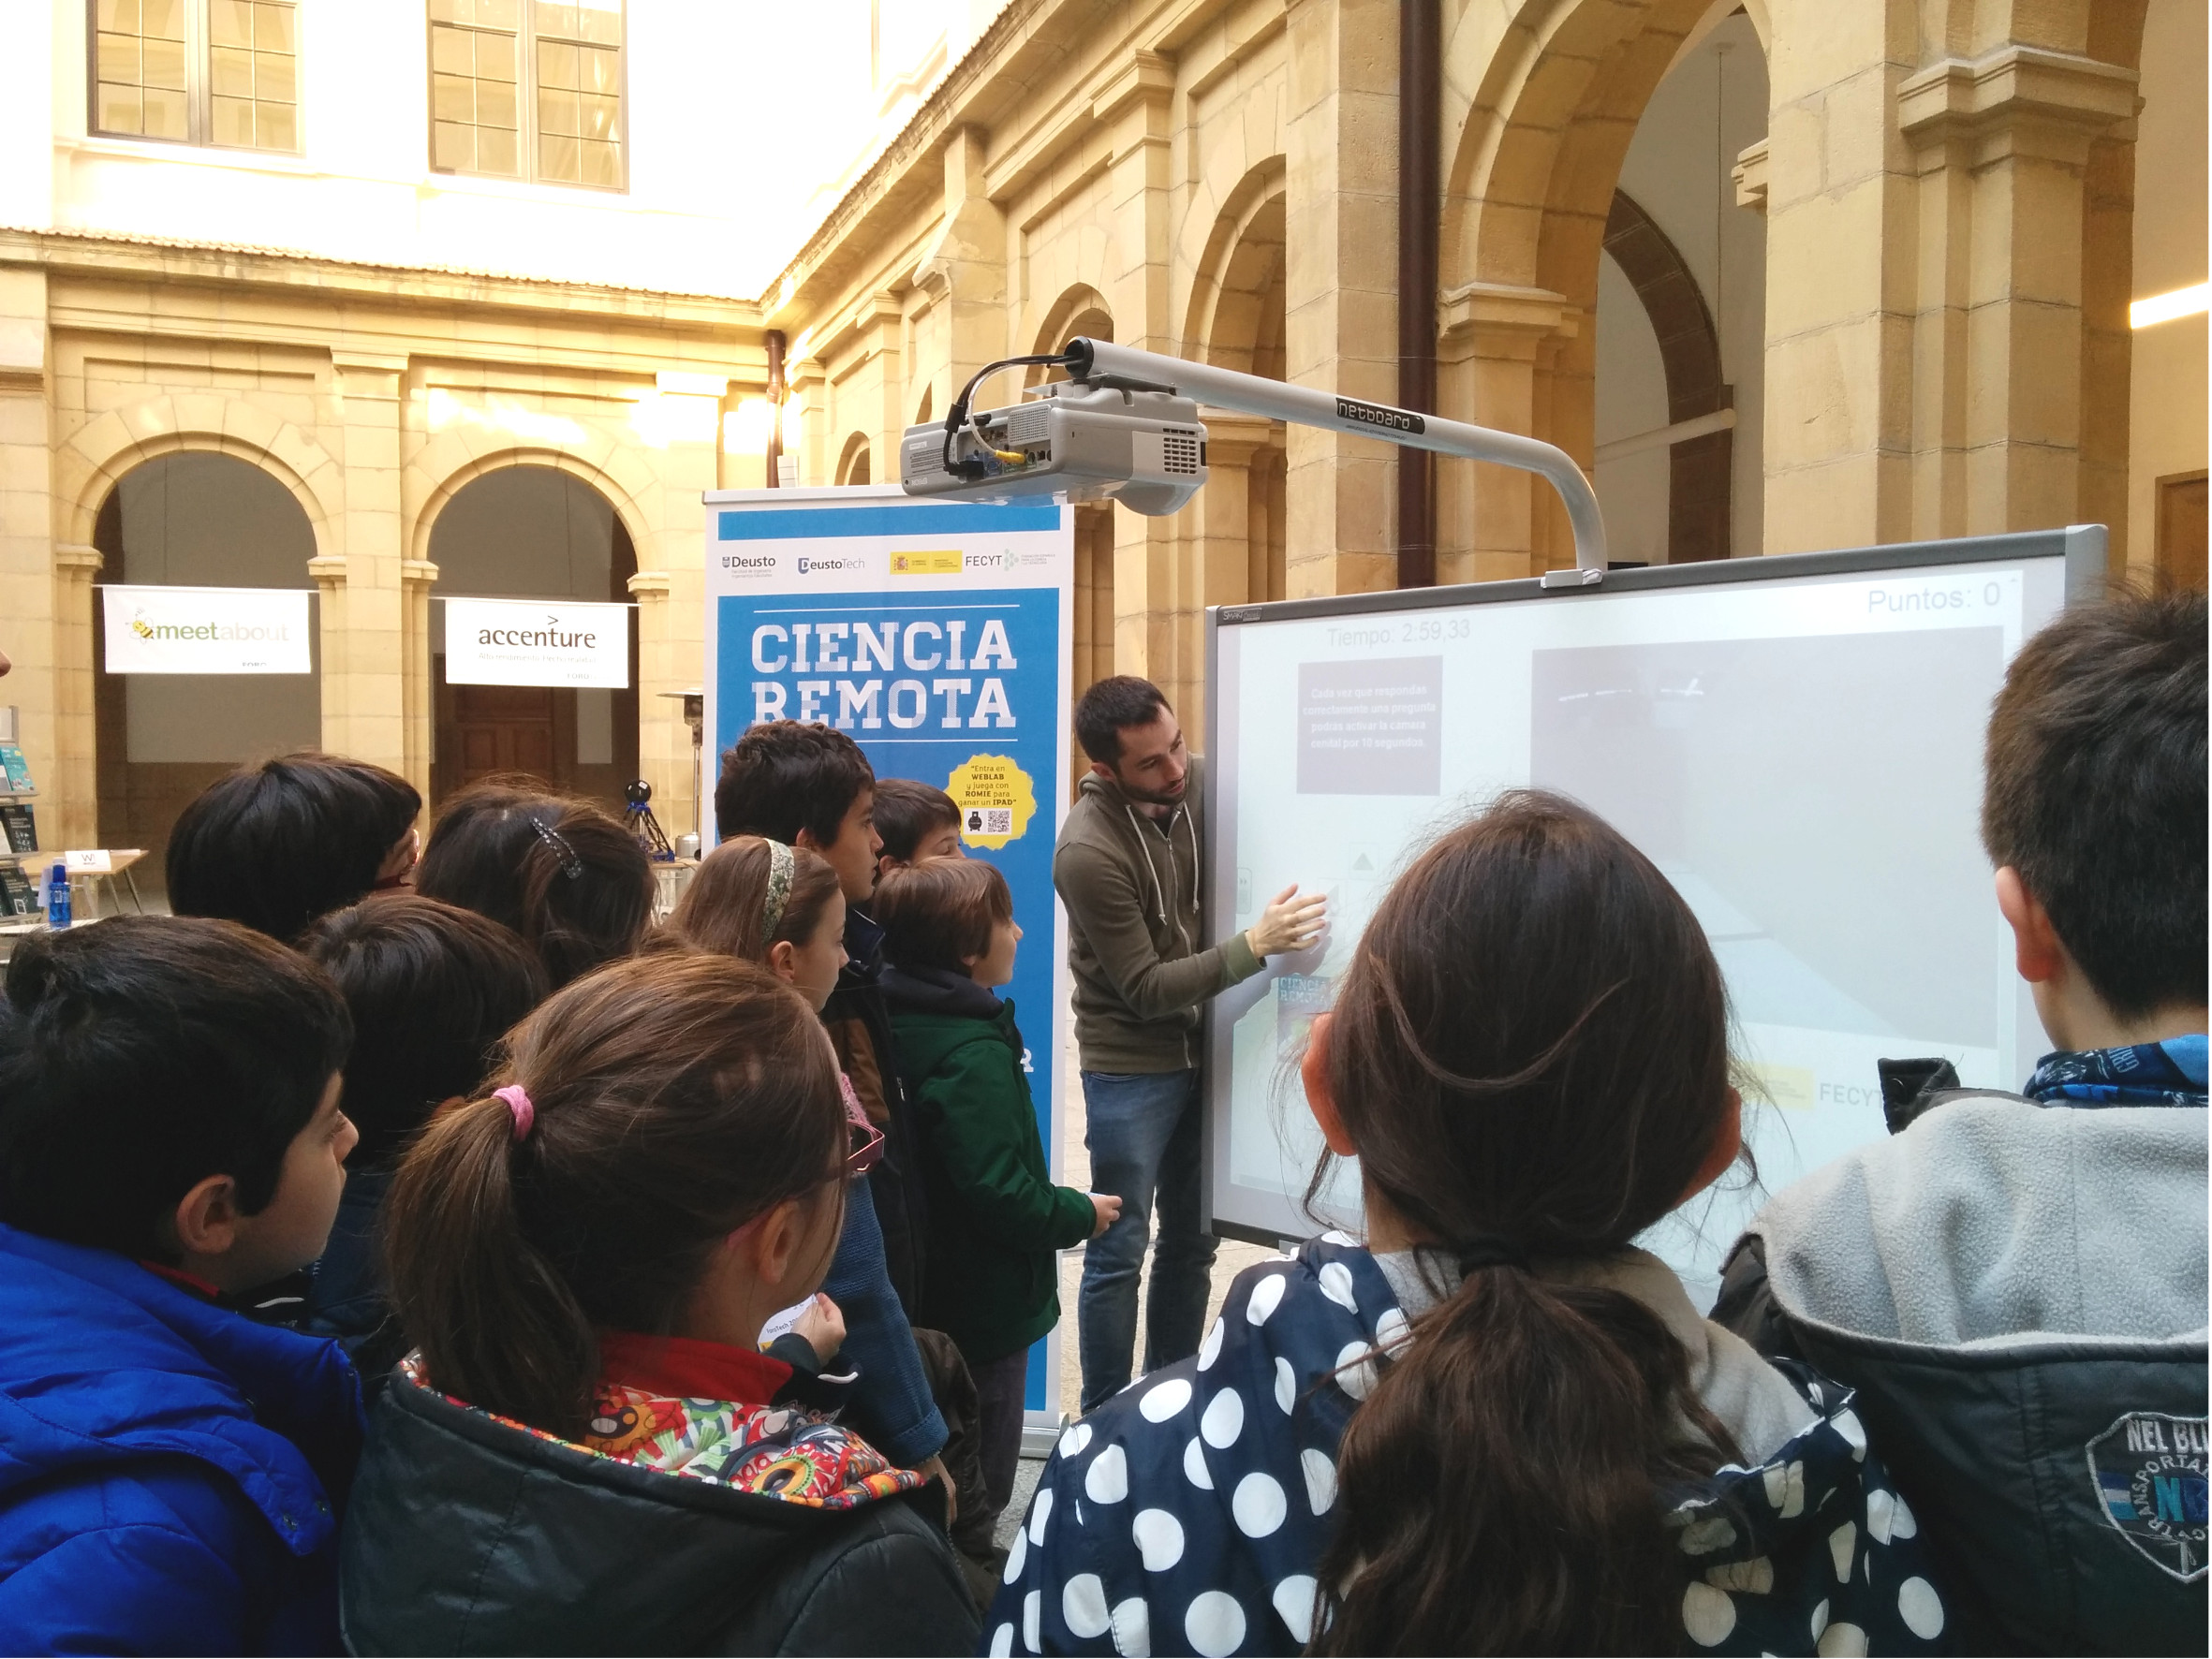
\includegraphics[height=0.3\textheight]{fig/forotech}
	\caption{Students looking at the ForoTech demonstration.}
	\label{fig:forotech}
\end{figure}

Moreover, 64 users logged in and played from home, with a total of 665 uses (more than 10 times per
user) with a total of 145,155.22 seconds of use (about 40 hours and 19 minutes), which is about
2,268 seconds per user or about 38 minutes.

The average game was of about 200 seconds (about 3 minutes and 20 seconds) and the day with most
uses was the Wednesday (the first day of use) in the afternoon, where the system had 164 uses. There
were no important issues with the robot, and most of them were hardware related, due to failing
pieces that were changed.

The final top ten ranking of the competition was the one in table~\ref{tab:ranking}. The first two
received an iPad (figure~\ref{fig:prizes}). There was a real competition where users were playing
until the last second of the competition, literally.

\begin{table}[ht]
	\centering
	\caption{Romie competition top ten ranking.}\label{tab:ranking}
	\begin{tabular}{ccc}
		\toprule
		\textbf{Name} & \emph{School} & \textbf{Points} \\
		\midrule
		Telmo		& Jesuitas					& 6,917,714	\\
		Hodei		& Jesuitas					& 6,915,484	\\
		Joshua		& El Regato					& 728,968	\\
		Martin		& Jesus María Bilbao		& 700,010	\\
		Adair		& Gurutzeta Eskola			& 589,400	\\
		Irune		& Jesuitas					& 578,420	\\
		Aitziber	& Jesuitas					& 464,070	\\
		Raul		& Fontal Somorrostro		& 456,865	\\
		Joseba		& Jesuitas					& 322,500	\\
		Antón		& Liceo Francés de Bilbao	& 221,520	\\
		\bottomrule
	\end{tabular}
\end{table}

\begin{figure}[ht]
	\centering
	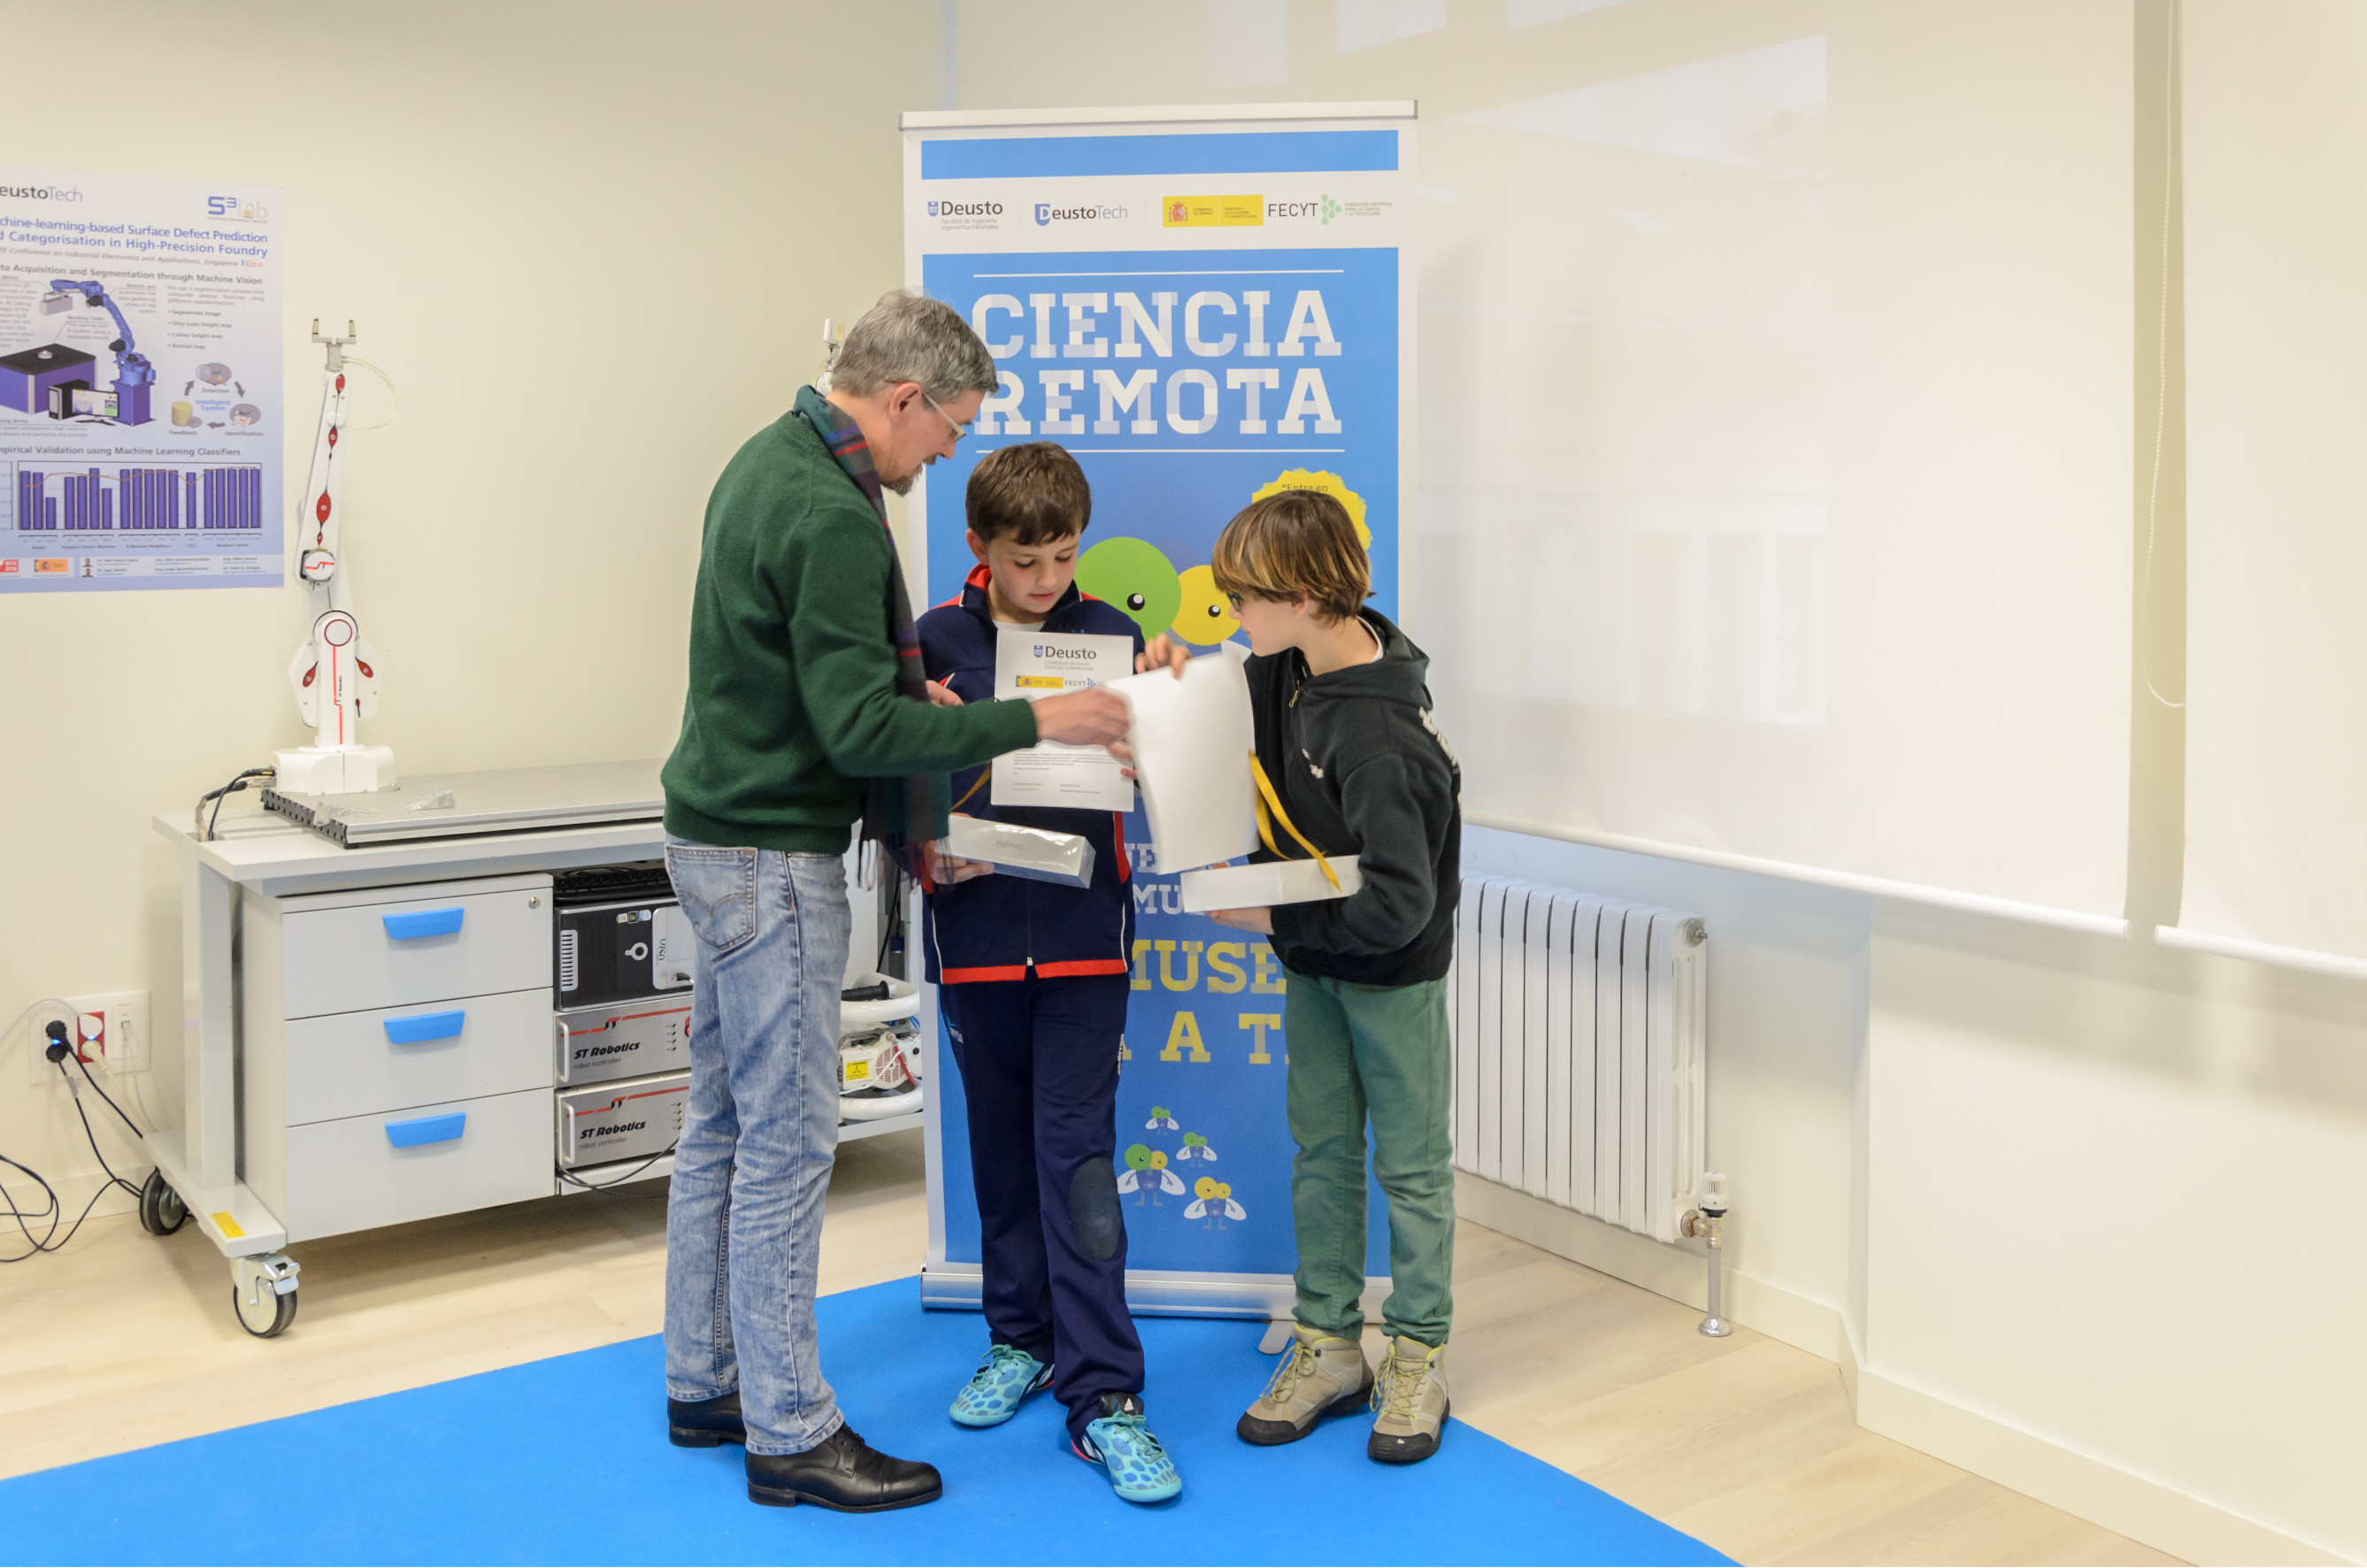
\includegraphics[height=0.3\textheight]{fig/prizes}
	\caption{Telmo and Hodei receiving the prize for wining the competition sponsored by \acrshort{fecyt}.}
	\label{fig:prizes}
\end{figure}

\section{Conclusions}

As it can be seen, the project has ended successfully, since it has fulfilled all the objectives
proposed at the beginning of it. The challenges have been difficult to complete but with hard work,
all of them have been successfully fulfilled.

The main outcomes for the platform have been that this project has a big potential. As it has been
demonstrated, it is easy to use, as it has been seen, since 64 users were able to play with it. This
fulfills the requirements of usability.

It has been integrated in the WebLab-Deusto platform, as the objectives demanded, which will allow
further use of the platform once the schools integrate it with their current use of WebLab-Deusto.

It has received a petition that will be made real for the end of 2015 of installing the game in
the Domus museum in A Coruña, Spain, under the ``Ciencia remota'' project of the \acrshort{fecyt}.
This fulfills the objective of disseminating the platform.

The two main environments of the platform have been developed and are fully functional. The game has
been tested with dozens of uses, while the visual programming \acrshort{ide} has shown great
potential on programming the robot with full control of the execution.

The usage statistics seen in the previous section were part of the objectives and show how the real
use of the platform has been. It has demonstrated the reliability of both the software and the
hardware of the platform as well as the viability for heavy load situations. In overall, the project
has demonstrated that it can be deployed in production, like it has been done in WebLab-Deusto.

\section{Future Lines of Work}

The current work is a complete system with its game modes. In WebLab-Deusto is currently deployed in
production, so it can be considered finished. Nevertheless, there are many ways that could lead to
improve both the user experience and the results of this project. For instance, here are a few that
could be developed in future research:

\begin{itemize}

	\item \textbf{Augmented reality}: The experiment could be equipped with augmented reality to give
	more interactivity to the user. It could show any sort of 3D game information in the labyrinth. Some
	scenarios have been suggested, such as a game where the user would have to recover things from the
	labyrinth moving across all of it and use them to build other hardware. The possibilities are
	unimaginable.

	\item \textbf{Computer vision}: Computer vision could be added to both top and on-board cameras.
	This way, the user and the software developed could have more information about the position of the
	robot or even about information in the labyrinth.

	It could help putting \acrshort{qr} or
	\acrlong{qr} codes in the walls to show something to the user. Moreover, top camera's computer
	vision could be used to locate the robot and try to challenge the user to move to a concrete place.

	\item \textbf{New game modes}: The platform currently provides a trivial type game, to which a
	psychological experiment can be added through configuration (is not enabled by default) and a visual
	programming \acrshort{ide}, where the user can program the robot. Nevertheless, these are only
	examples of the potential of this project.

	The platform is prepared, thanks to its modular \acrshort{api}s to host more experiments and games
	that could use it. It could be used for teaching, for experimenting with art (painting the walls or
	asking the user to paint patterns with the robot movement) or for any other use the imagination can
	lead us to.

\end{itemize}

In any case, the current platform is extensible enough to allow all kind of experiment development,
also allowing for remote deployments of more experiments like this one. In this case, there is
already a plan to deploy the experiment in the Domus museum in A Coruña, Spain. This way, the big
potential of the project is demonstrated, as well as its future lines of work, that can lead it to
be used in many scopes.


\printbibliography[heading=bibintoc]
\printglossary[type=\acronymtype]

\appendix

\chapter*{Acknowledgements}
\addcontentsline{toc}{chapter}{Acknowledgements}

I would like to thank the following people for their help, since without them this project would not
have been possible. Thanks to them I was able to life this amazing experience.

\begin{itemize}
	\item \textbf{My mum, Arantza}, for dedicating her last days of her life to support me when I
	was starting my first months of my degree, and for being the best mother any kid could dream of.

	\item \textbf{My dad, Manu}, for being patient with me all these years and giving me the
	opportunity to continue my studies by giving me moral and financial support.

	\item \textbf{Javier García Zubía}, for being the tutor of this project and for giving me the
	opportunity to learn while working in WebLab-Deusto for the last two years.

	\item \textbf{Pablo Garaizar}, for recommending me to Javier García Zubía as a
	potential candidate to work in WebLab-Deusto.

	\item \textbf{Pablo Orduña}, for letting me understand \textit{his} WebLab-Deusto and helping me
	each time I had issues in my development.

	\item \textbf{Luis Rodríguez}, for being incredibly patient with all my questions, that were not
	few.

	\item \textbf{Gabriel Martinez}, for having him in WebLab-Deusto and for being a good co-worker.
	His contributions to the AI of the robot were priceless.

	\item \textbf{Ignacio Angulo}, for helping me with the electronics of the robot. I was able to
	learn a lot with him.
\end{itemize}

\chapter*{Acknowledgements}
\addcontentsline{toc}{chapter}{Acknowledgements}

Me gustaría agradecer a las siguientes personas por su ayuda, ya que sin ellas este proyecto no
habría sido posible. Gracias a ellos pude vivir esta asombrosa experiencia.

\begin{itemize}
	\item \textbf{Mi madre, Arantza}, por dedicar sus últimos días de su vida a apoyarme cuando
	comenzaba mis primeros meses de carrera, y por ser la mejor madre que ningún niño podría soñar.

	\item \textbf{Mi padre, Manu}, por ser paciente conmigo todos estos años y haberme dado la
	oportunidad de continuar mis estudios dándome a su apoyo moral y financiero.

	\item \textbf{Javier García Zubía}, por ser el tutor de este proyecto y por darme la oportunidad
	de aprender mientras trabajaba en WebLab-Deusto los últimos dos años.

	\item \textbf{Pablo Garaizar}, por recomendarme a Javier García Zubía como un candidato
	potencial para trabajar en WebLab-Deusto.

	\item \textbf{Pablo Orduña}, por permitirme entender \textit{su} WebLab-Deusto y ayudarme cada
	vez que tenía problemas con el desarrollo.

	\item \textbf{Luis Rodríguez}, por ser increíblemente paciente con todas mis preguntas, que no
	fueron pocas.

	\item \textbf{Gabriel Martinez}, por tenerlo en WebLab-Deusto y ser un buen compañero de
	trabajo. Sus contribuciones a la IA del robot fueron impagables.

	\item \textbf{Ignacio Angulo}, por ayudarme con las electrónicas del robot. Con el pude aprender
	mucho.
\end{itemize}


\backmatter

\end{document}
